\section{CMMR spacetime}

We will now perform an analysis similar to that of the previous section but using the solution class found by Cabrera-Munguia, Manko and Ruiz (CMMR). This metric describes a pair of static Kerr black holes and thus we will show that one can extract rotational energy from the system using geodesic motion.

\subsection{Spacetime metric}

In Weyl's cylindrical coordinates, the CMMR line element reads
%
\begin{equation}
  \ud s^2 = -f(\rho,z)\left[\ud t - \omega(\rho,z)\ud\varphi\right]^2 \\
  + f(\rho,z)^{-1}\left[e^{2\gamma(\rho,z)}\left(\ud \rho^2 + \ud z^2\right) + \rho^2\ud\varphi^2\right]
  \label{ch:penrose_binaries/eq:line_element}
\end{equation}
%
where the real valued functions $f(\rho,z)$, $\omega(\rho,z)$ and $\exp[2\gamma(\rho,z)]$ were implemented as described in Sec.~IV of Ref.~\cite{MANKO2020}. We shall not reproduce these functions here as they take a few pages worth of equations.

This solution is characterized by a set five parameters: The masses of the Kerr constituents $m_1$ and $m_2$, their angular momenta per unit mass $a_1$ and $a_2$ and the coordinate distance between the centers of the two black holes $R$. In Weyl's coordinates, each horizon is a line that extends over the $z$ axis centered around $z=\pm R/2$ (See Fig.~3 of Ref.~\cite{MANKO2020}). In order to work with dimensionless quantities, we will introduce the three additional parameters given in terms of the preceding five. The first is the total mass of the system $M$, given by
%
\begin{equation}
  M = m_1 + m_2.
  \label{ch:penrose_binaries/eq:total_mass_def}
\end{equation}
%
The second is the system's mass ratio $q$ given by
%
\begin{equation}
  q = \frac{m_1}{m_2}
  \label{ch:penrose_binaries/eq:mass_ratio_def}
\end{equation}
%
and finally, the third is a dimensionless distance parameter $b$ given by
%
\begin{equation}
  b = \frac{M}{R}.
  \label{ch:penrose_binaries/eq:dist_param_def}
\end{equation}

By performing the coordinate transformation
%
\begin{equation}
  x^{\mu} \rightarrow \frac{x^\mu}{M}
  \label{ch:penrose_binaries/eq:coord_transf_dimensionless}
\end{equation}
%
where the $x^\mu$ are the space-time coordinates, we effectively rescale the metric functions $f$, $\omega$ and $e^{2\gamma}$ by a factor of $1/M$ and as a result they become dimensionless quantities with the added benefit that the space-time coordinates $t$, $\rho$, $z$ and $\varphi$ are also dimensionless quantities.

If additionally we fixate $M$ to be unitary, we can fully describe the CMMR metric by specifying four dimensionless parameters $q$, $b$, $a_1$ and $a_2$ from which all necessary quantities appearing in the metric functions can be calculated. Explicitly, we can write the inverse relations
%
\begin{equation}
  m_1 = \frac{Mq}{1+q},
  \label{ch:penrose_binaries/eq:m1_from_q}
\end{equation}
%
\begin{equation}
  m_2 = \frac{M}{1+q}
  \label{ch:penrose_binaries/eq:m2_from_q}
\end{equation}
%
and
\begin{equation}
  R = \frac{M}{b}.
  \label{ch:penrose_binaries/eq:r_from_b}
\end{equation}

The CMMR solution when written in the form given by Ref.~\cite{MANKO2020} can appropriately describe not only a ``standard'' Kerr black hole binary but also extreme and naked Kerr sources, depending on the values chosen for the solution's parameters. In order to study scenarios of greater astrophysical relevance we shall limit ourselves to discussions pertaining only to the black hole sector of the metric which is given by the set of parameters that cause the constituent black holes horizons half lengths (the expressions for $\sigma_1$ and $\sigma_2$ after Eq. (18) of Ref.~\cite{MANKO2020}) to be real valued and greater than zero. By choosing values of $q$ and $b$, we are able to determine which values of $a_1$ and $a_2$ represent black hole binary solutions. The results are presented in Fig.~\ref{ch:penrose_binaries/fig:parameter_space}. For each $q$ and $b$ pair, a blue shape represents the region of $a_1$ and $a_2$ values representing black hole configurations.

\begin{figure}
  \centering
  \subfloat[$b=0.1$, $q=0.1$]{
    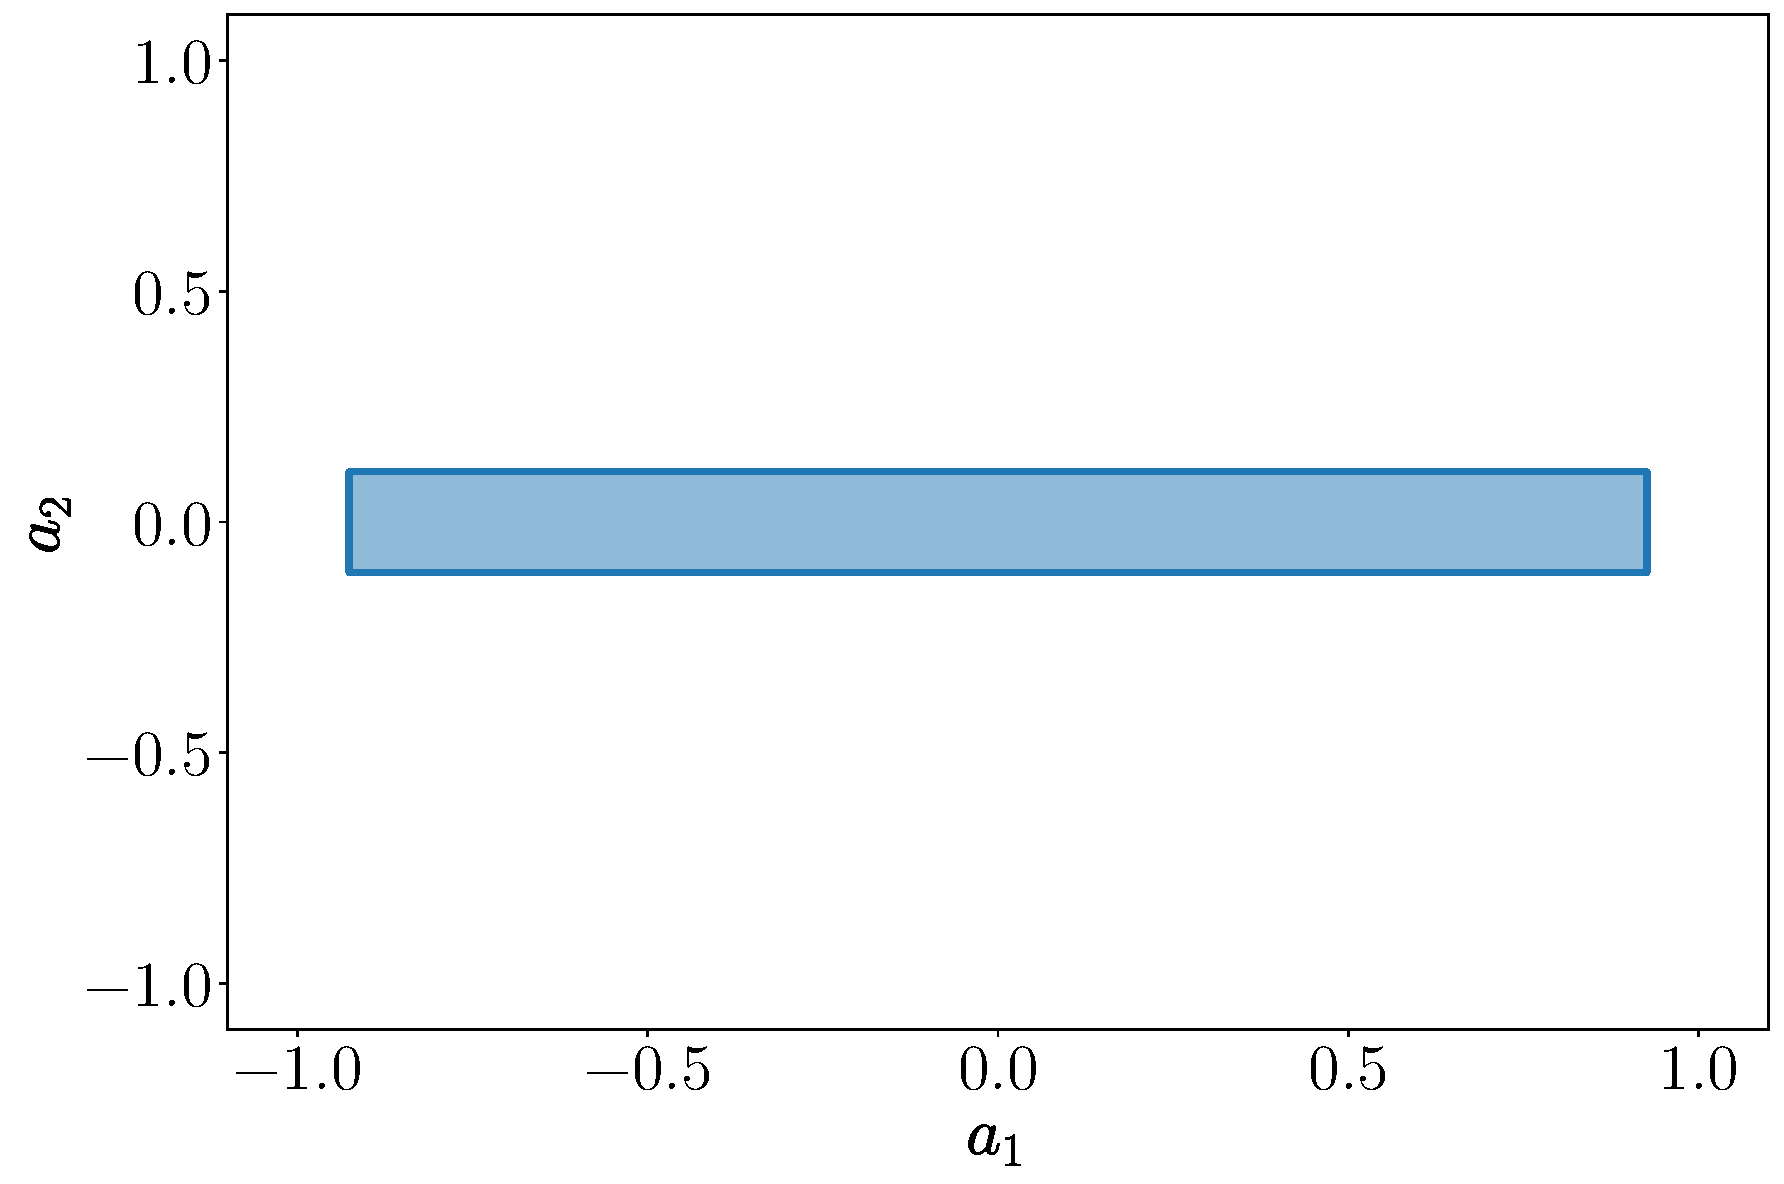
\includegraphics[scale = 0.15]{img/penrose_binaries/cmmr_par_region/par_region_b_0.1_q_0.1.pdf}
    \label{ch:penrose_binaries/fig:par_reg_a}
  }
  \subfloat[$b=0.1$, $q=0.5$]{
    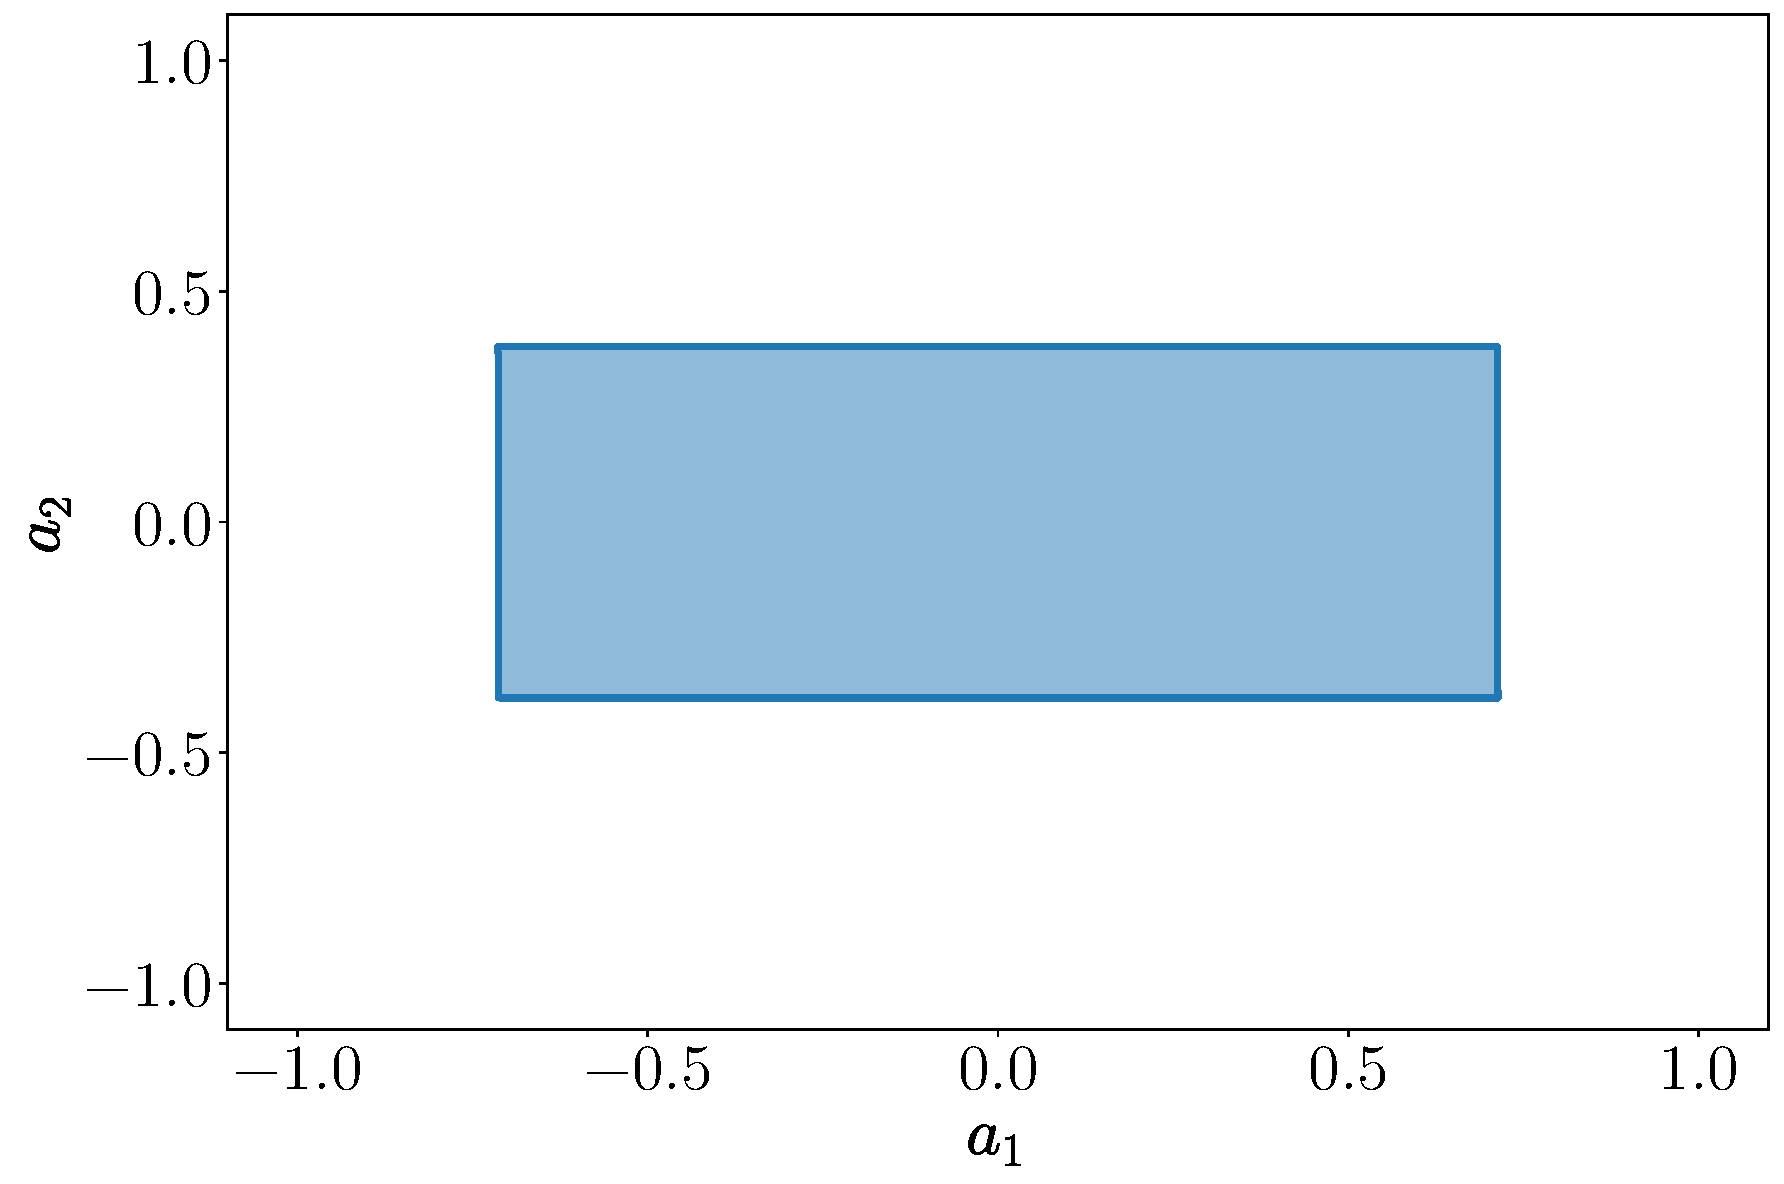
\includegraphics[scale = 0.15]{img/penrose_binaries/cmmr_par_region/par_region_b_0.1_q_0.5.pdf}
    \label{ch:penrose_binaries/fig:par_reg_b}
  }
  \subfloat[$b=0.1$, $q=1.0$]{
    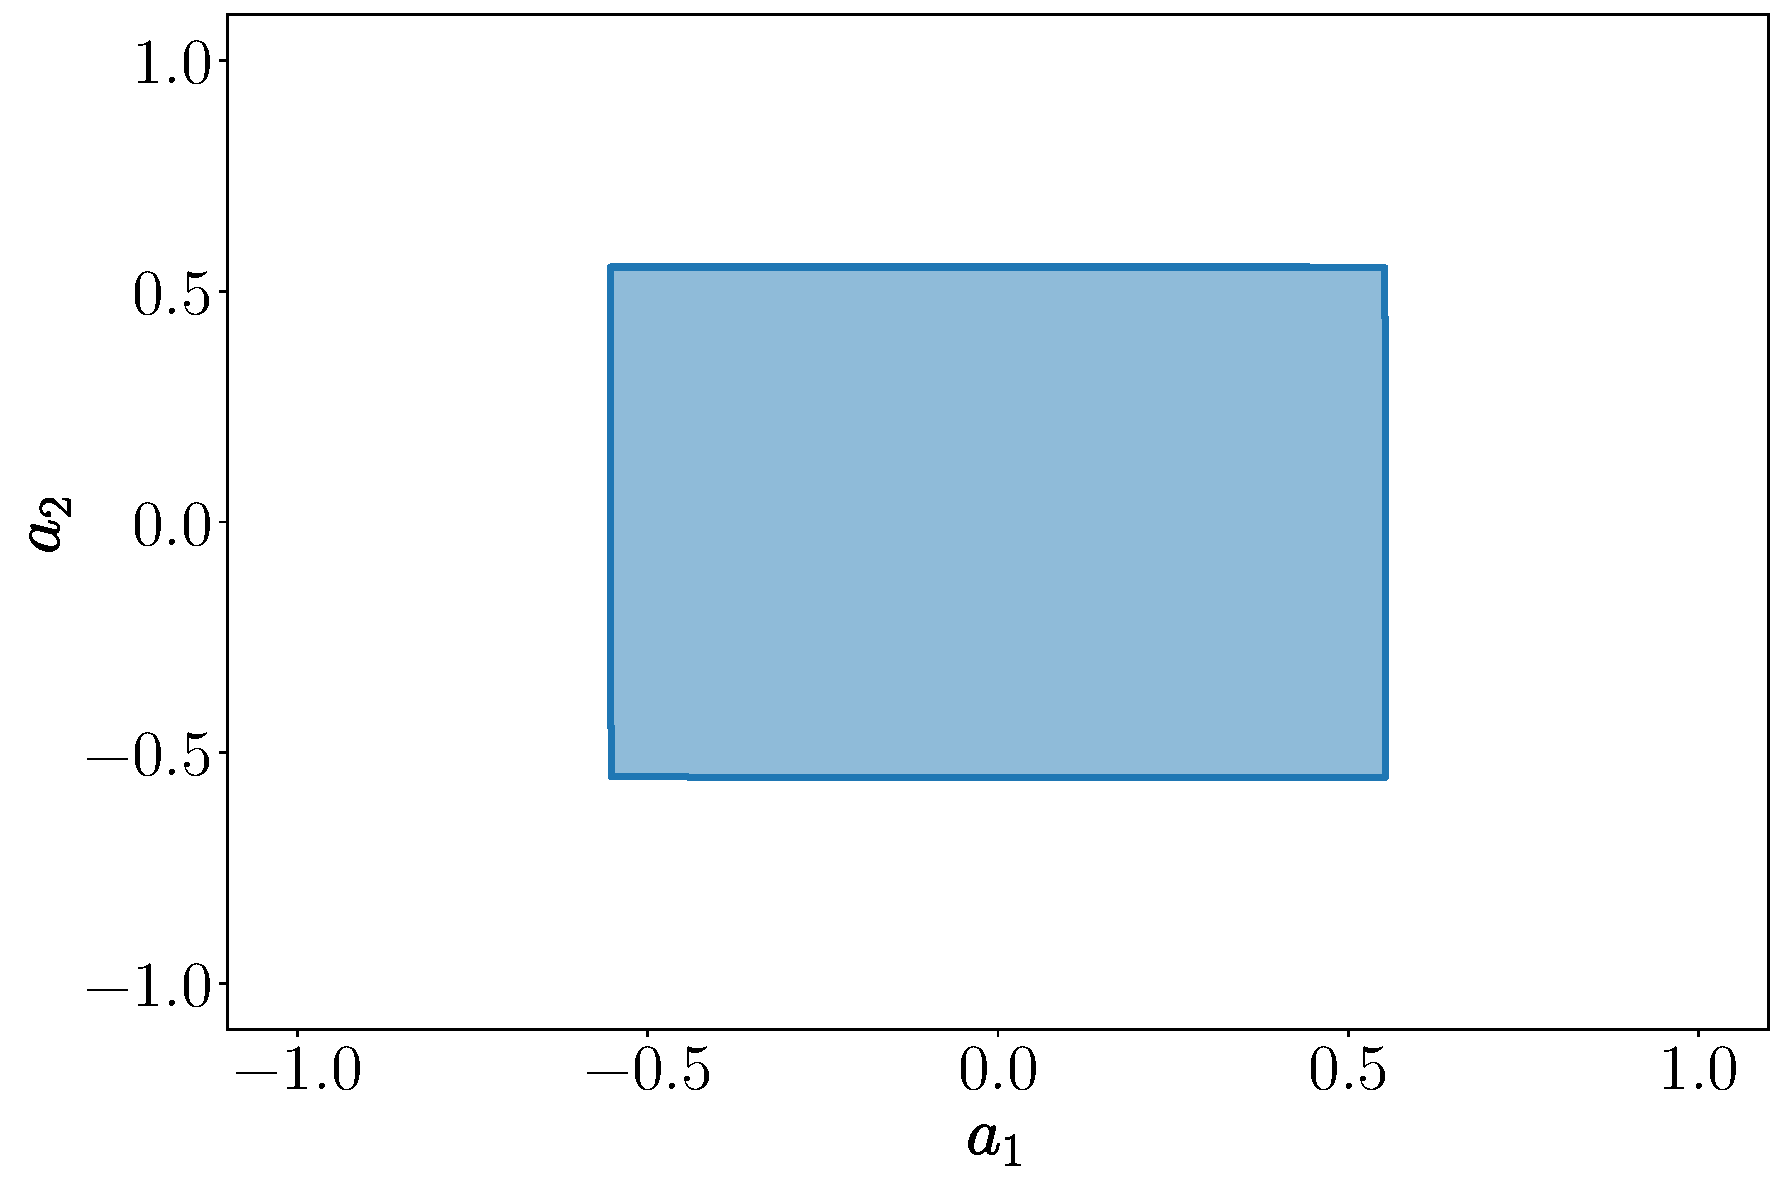
\includegraphics[scale = 0.15]{img/penrose_binaries/cmmr_par_region/par_region_b_0.1_q_1.0.pdf}
    \label{ch:penrose_binaries/fig:par_reg_c}
  }
  \newline
  \subfloat[$b=0.5$, $q=0.1$]{
    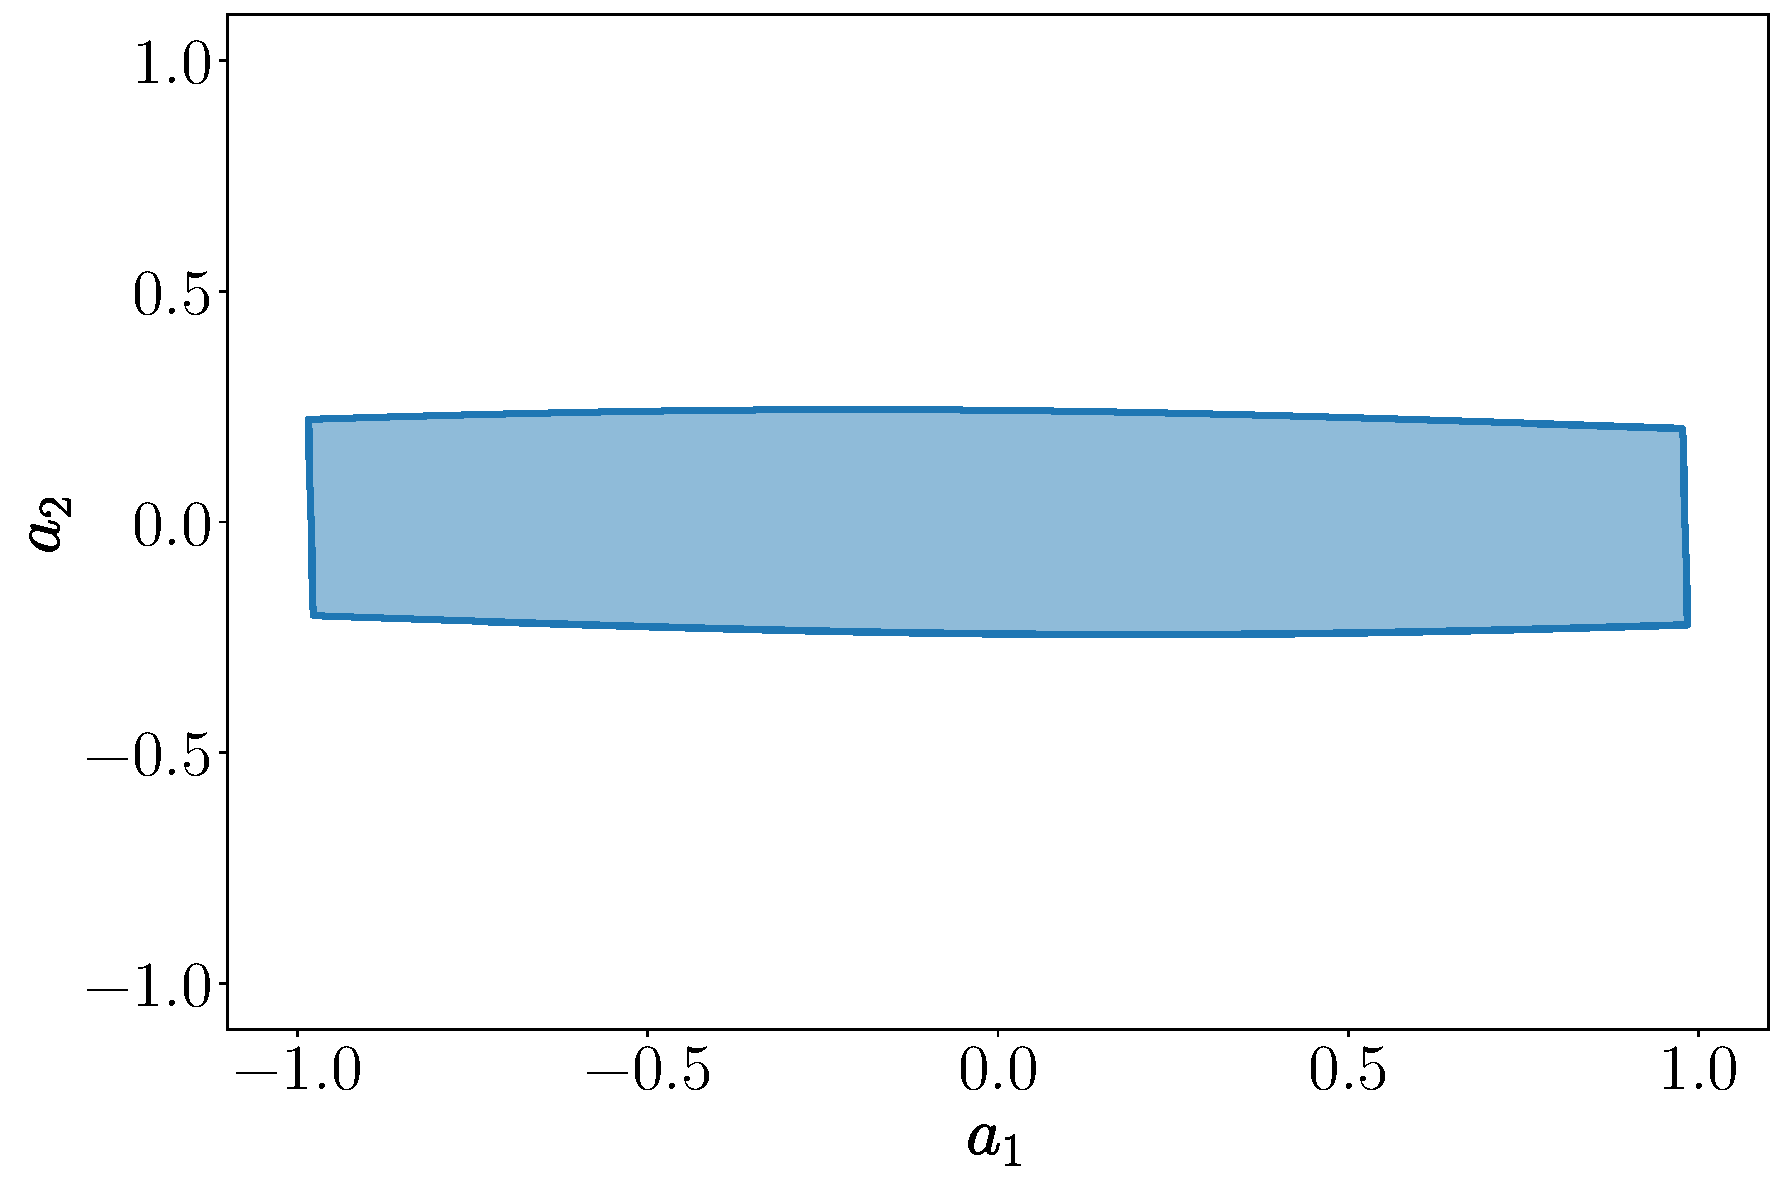
\includegraphics[scale = 0.15]{img/penrose_binaries/cmmr_par_region/par_region_b_0.5_q_0.1.pdf}
    \label{ch:penrose_binaries/fig:par_reg_d}
  }
  \subfloat[$b=0.5$, $q=0.5$]{
    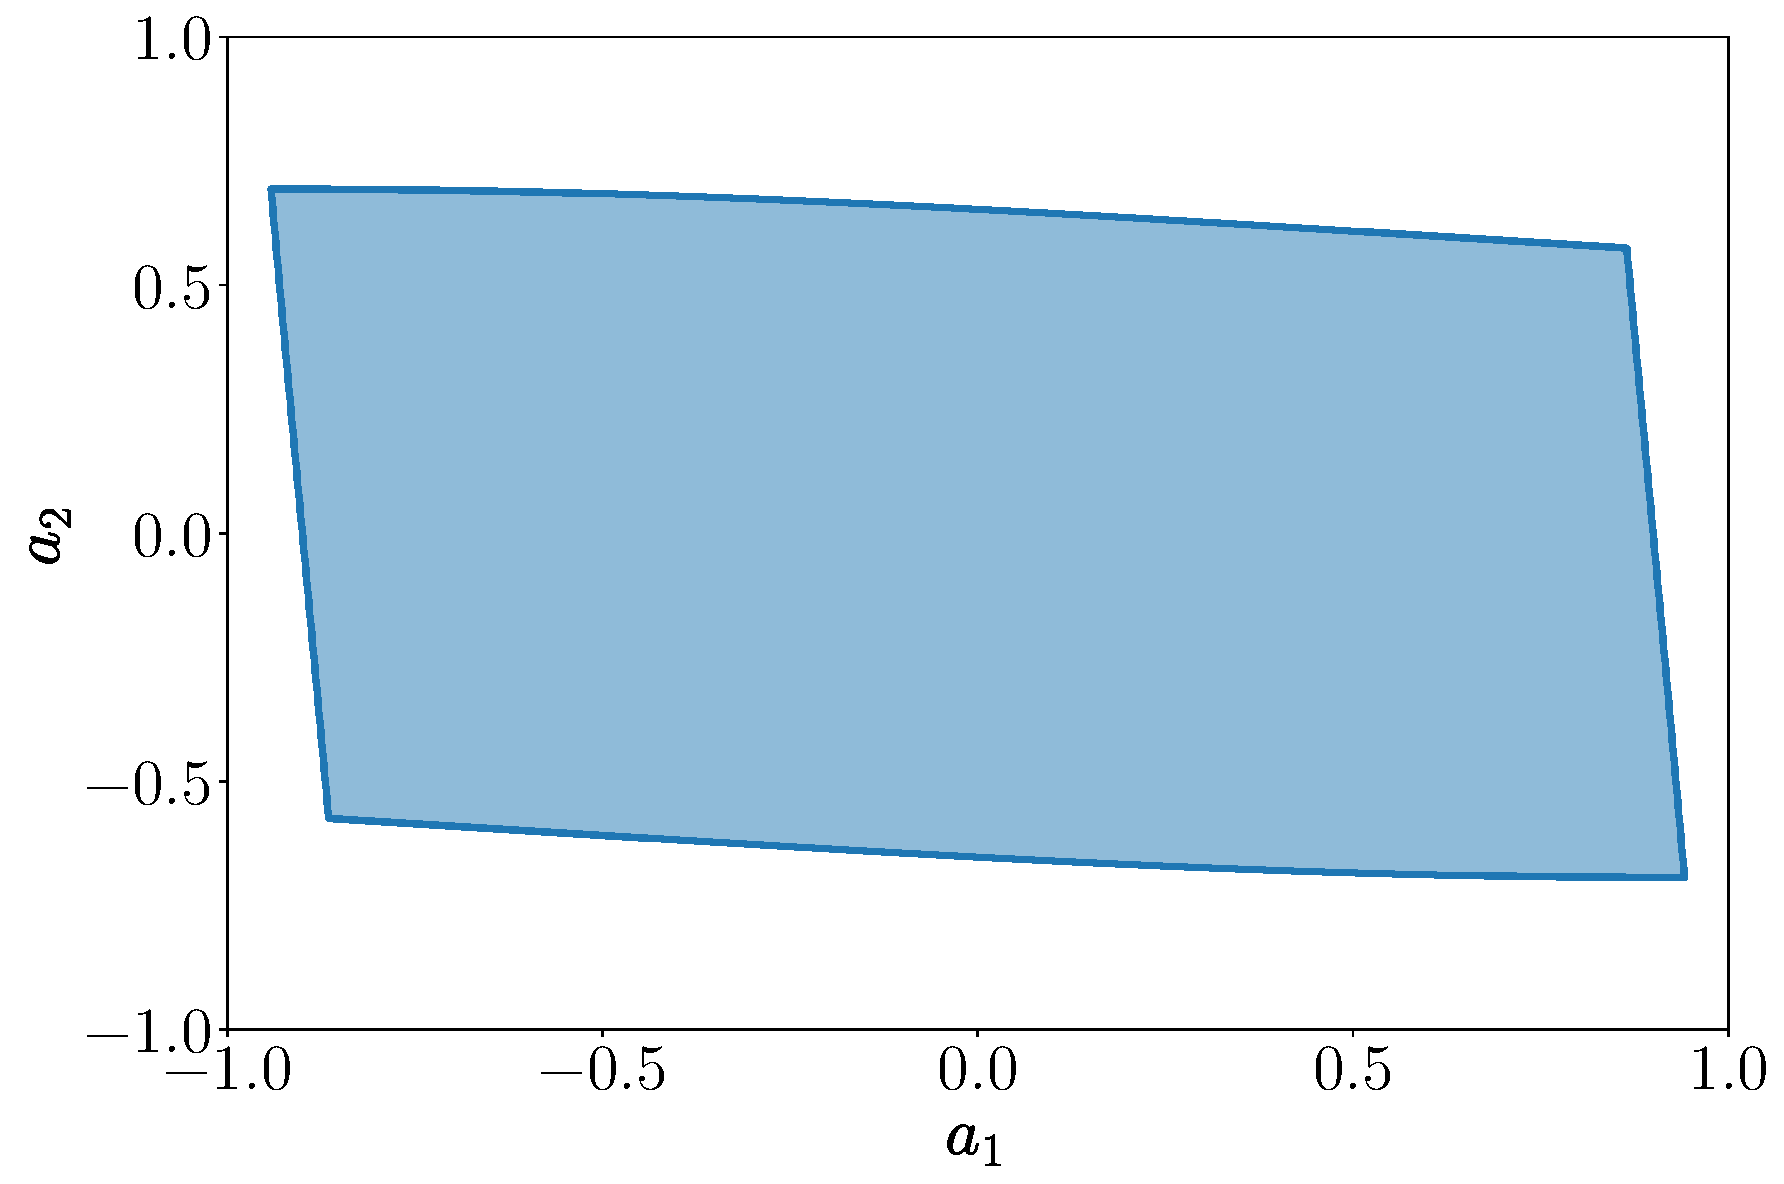
\includegraphics[scale = 0.15]{img/penrose_binaries/cmmr_par_region/par_region_b_0.5_q_0.5.pdf}
    \label{ch:penrose_binaries/fig:par_reg_e}
  }
  \subfloat[$b=0.5$, $q=1.0$]{
    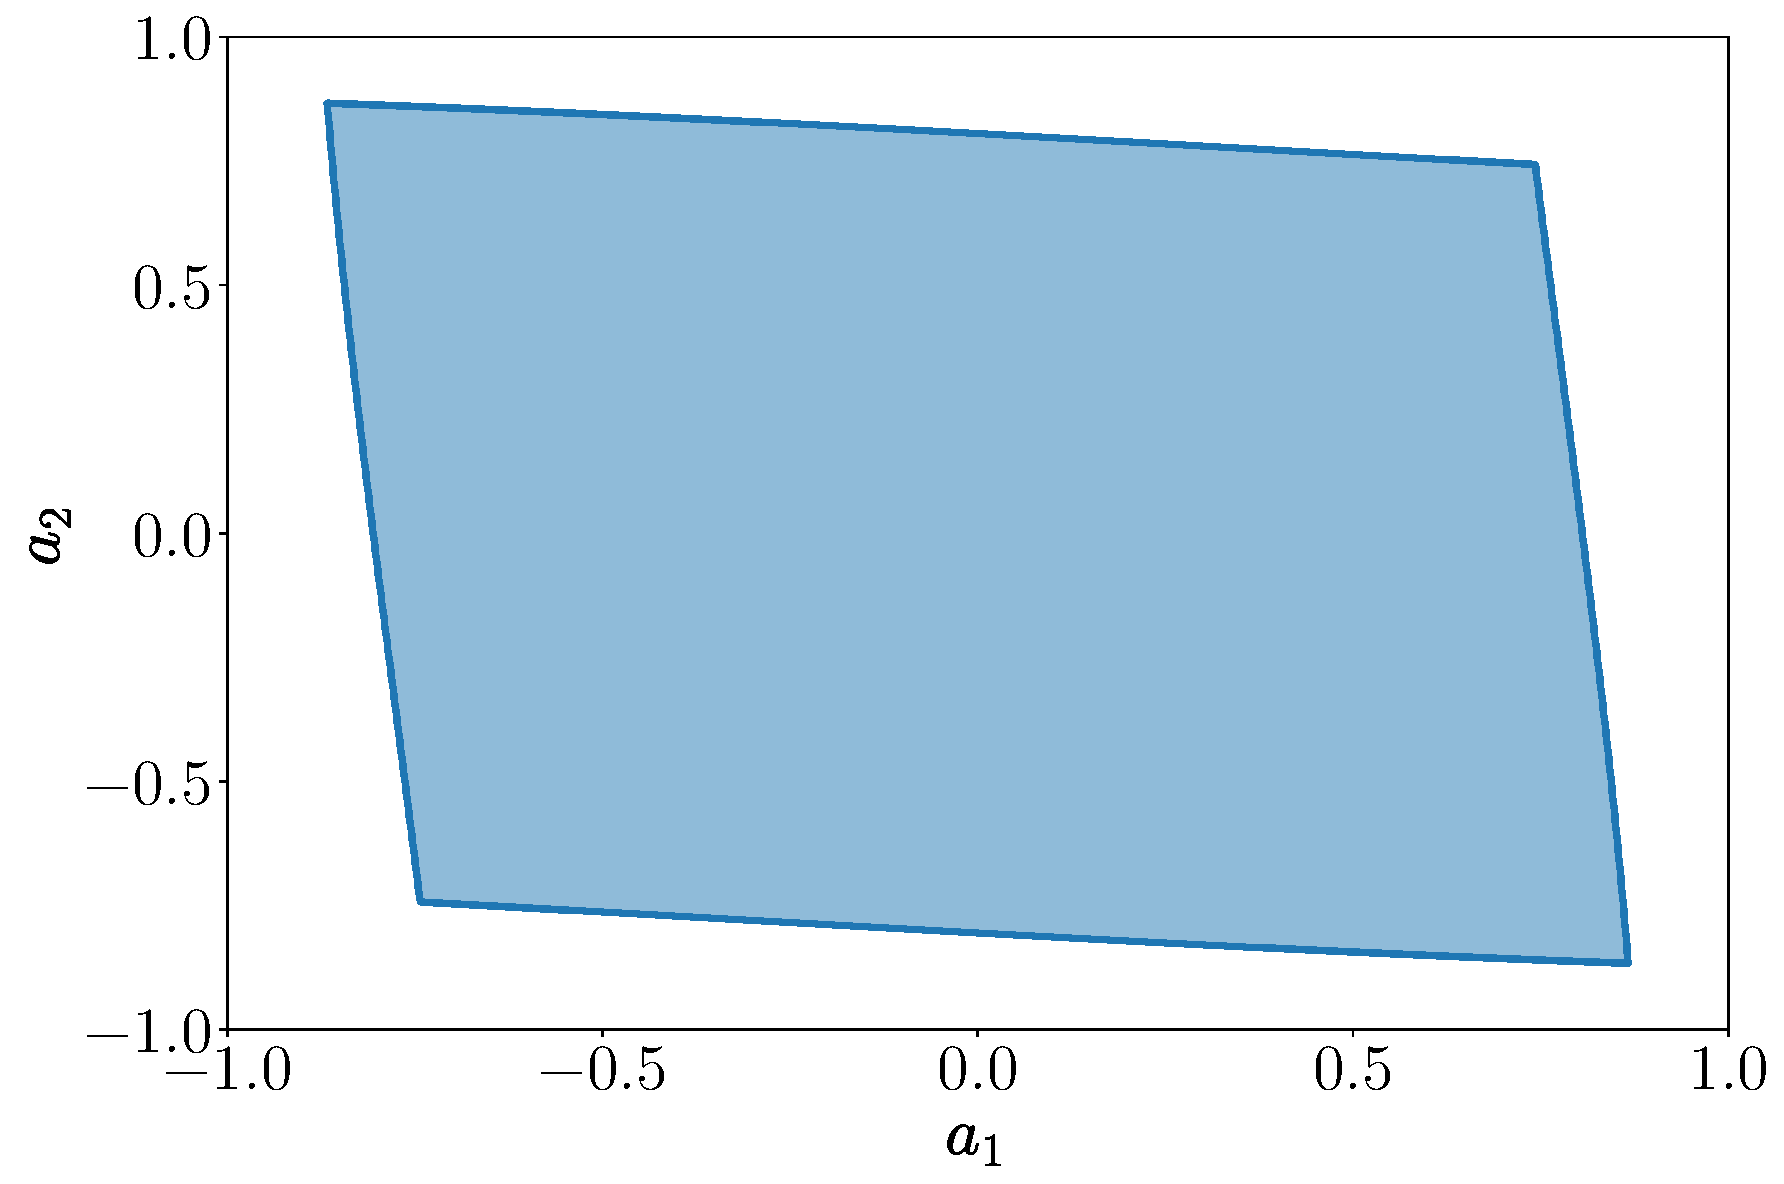
\includegraphics[scale = 0.15]{img/penrose_binaries/cmmr_par_region/par_region_b_0.5_q_1.0.pdf}
    \label{ch:penrose_binaries/fig:par_reg_f}
  }
  \newline
  \subfloat[$b=0.98$, $q=0.1$]{
    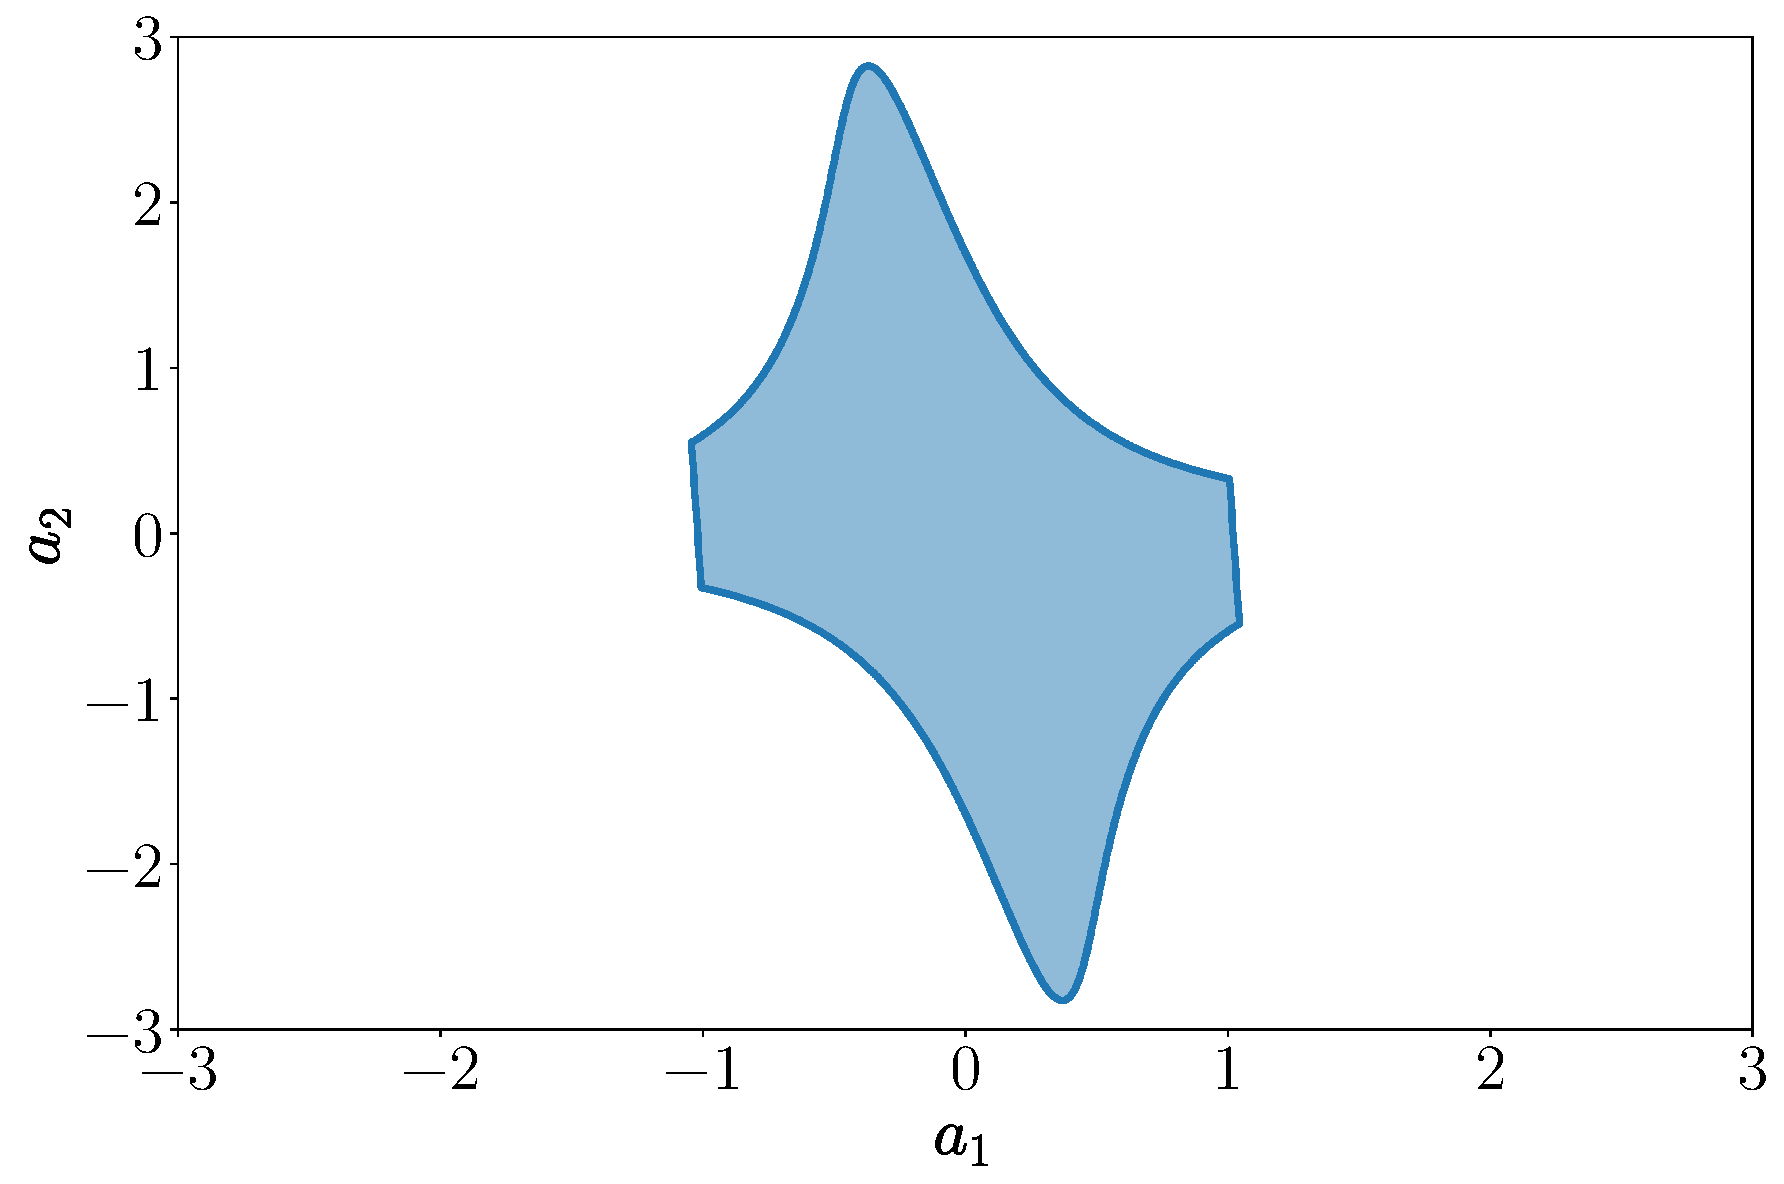
\includegraphics[scale = 0.15]{img/penrose_binaries/cmmr_par_region/par_region_b_0.98_q_0.1.pdf}
    \label{ch:penrose_binaries/fig:par_reg_g}
  }
  \subfloat[$b=0.98$, $q=0.5$]{
    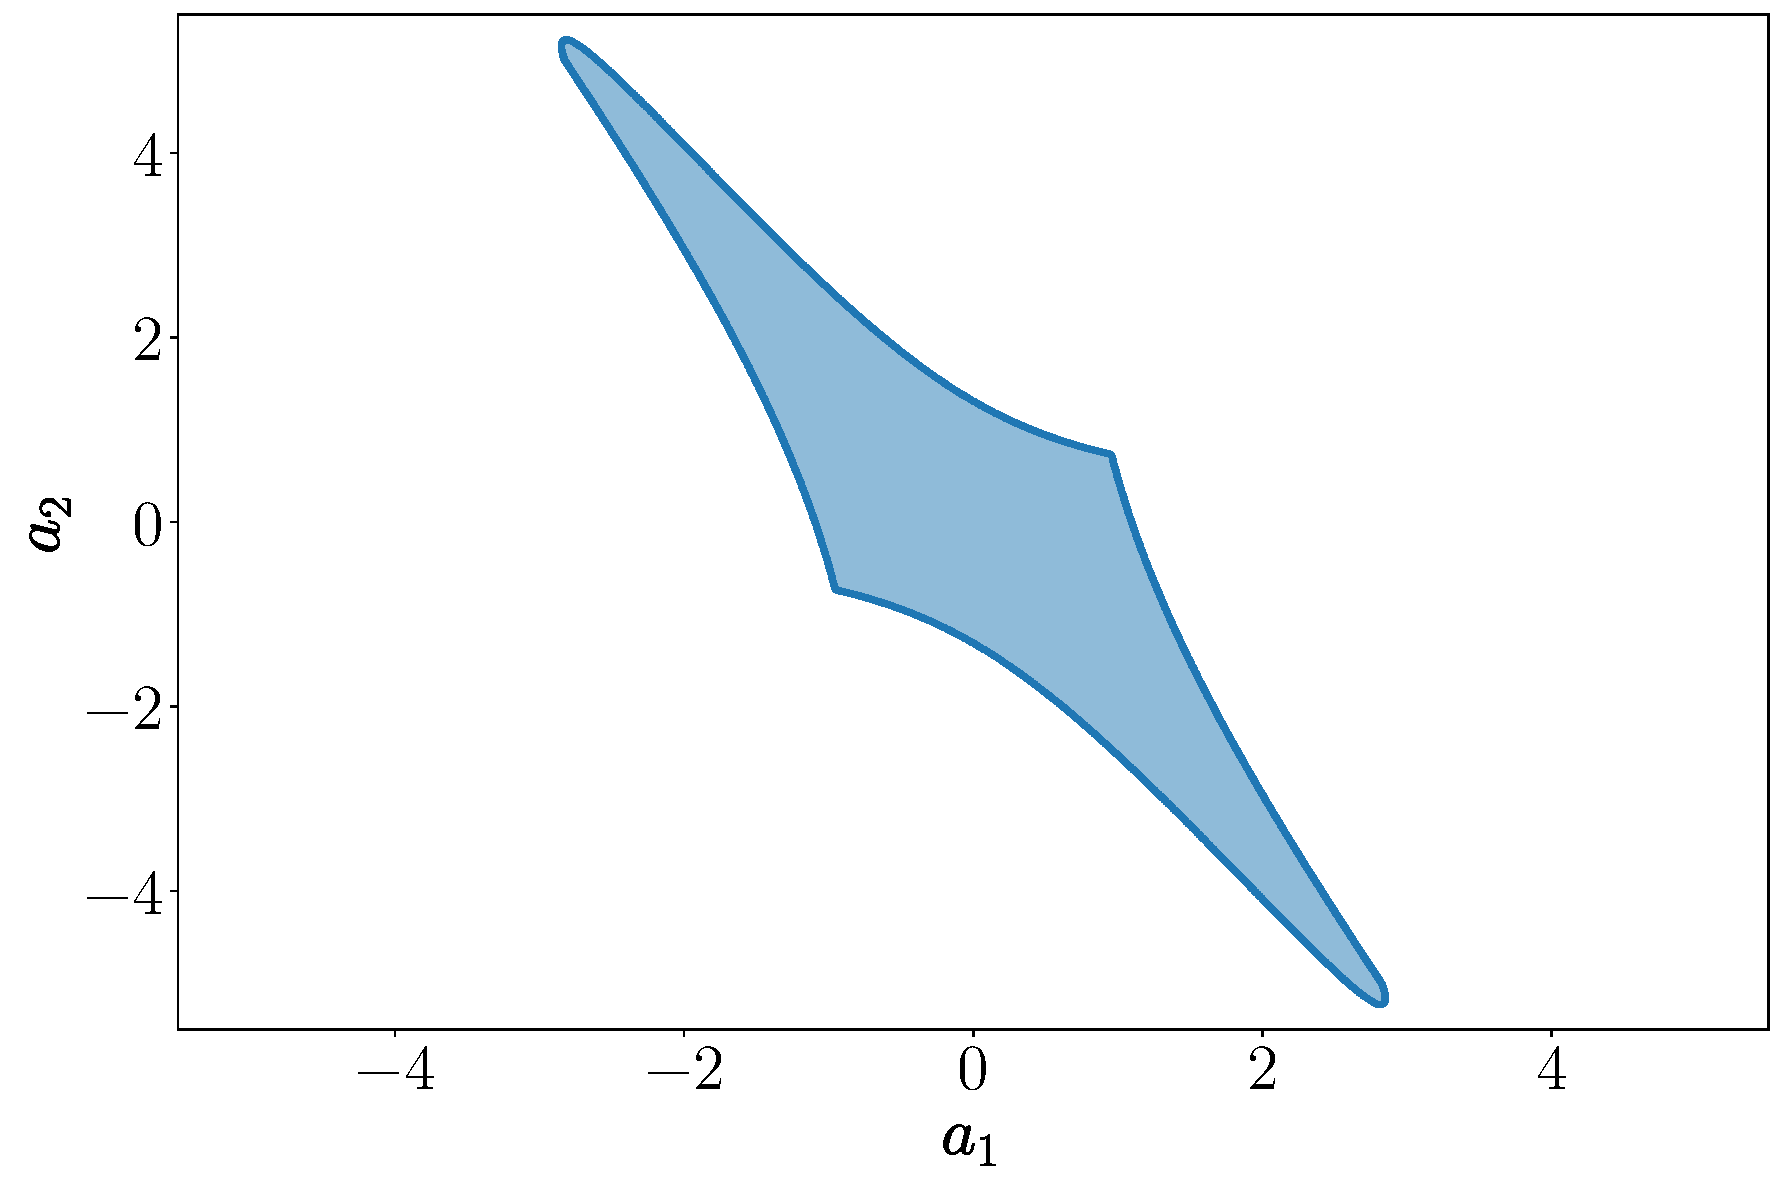
\includegraphics[scale = 0.15]{img/penrose_binaries/cmmr_par_region/par_region_b_0.98_q_0.5.pdf}
    \label{ch:penrose_binaries/fig:par_reg_h}
  }
  \subfloat[$b=0.98$, $q=1.0$]{
    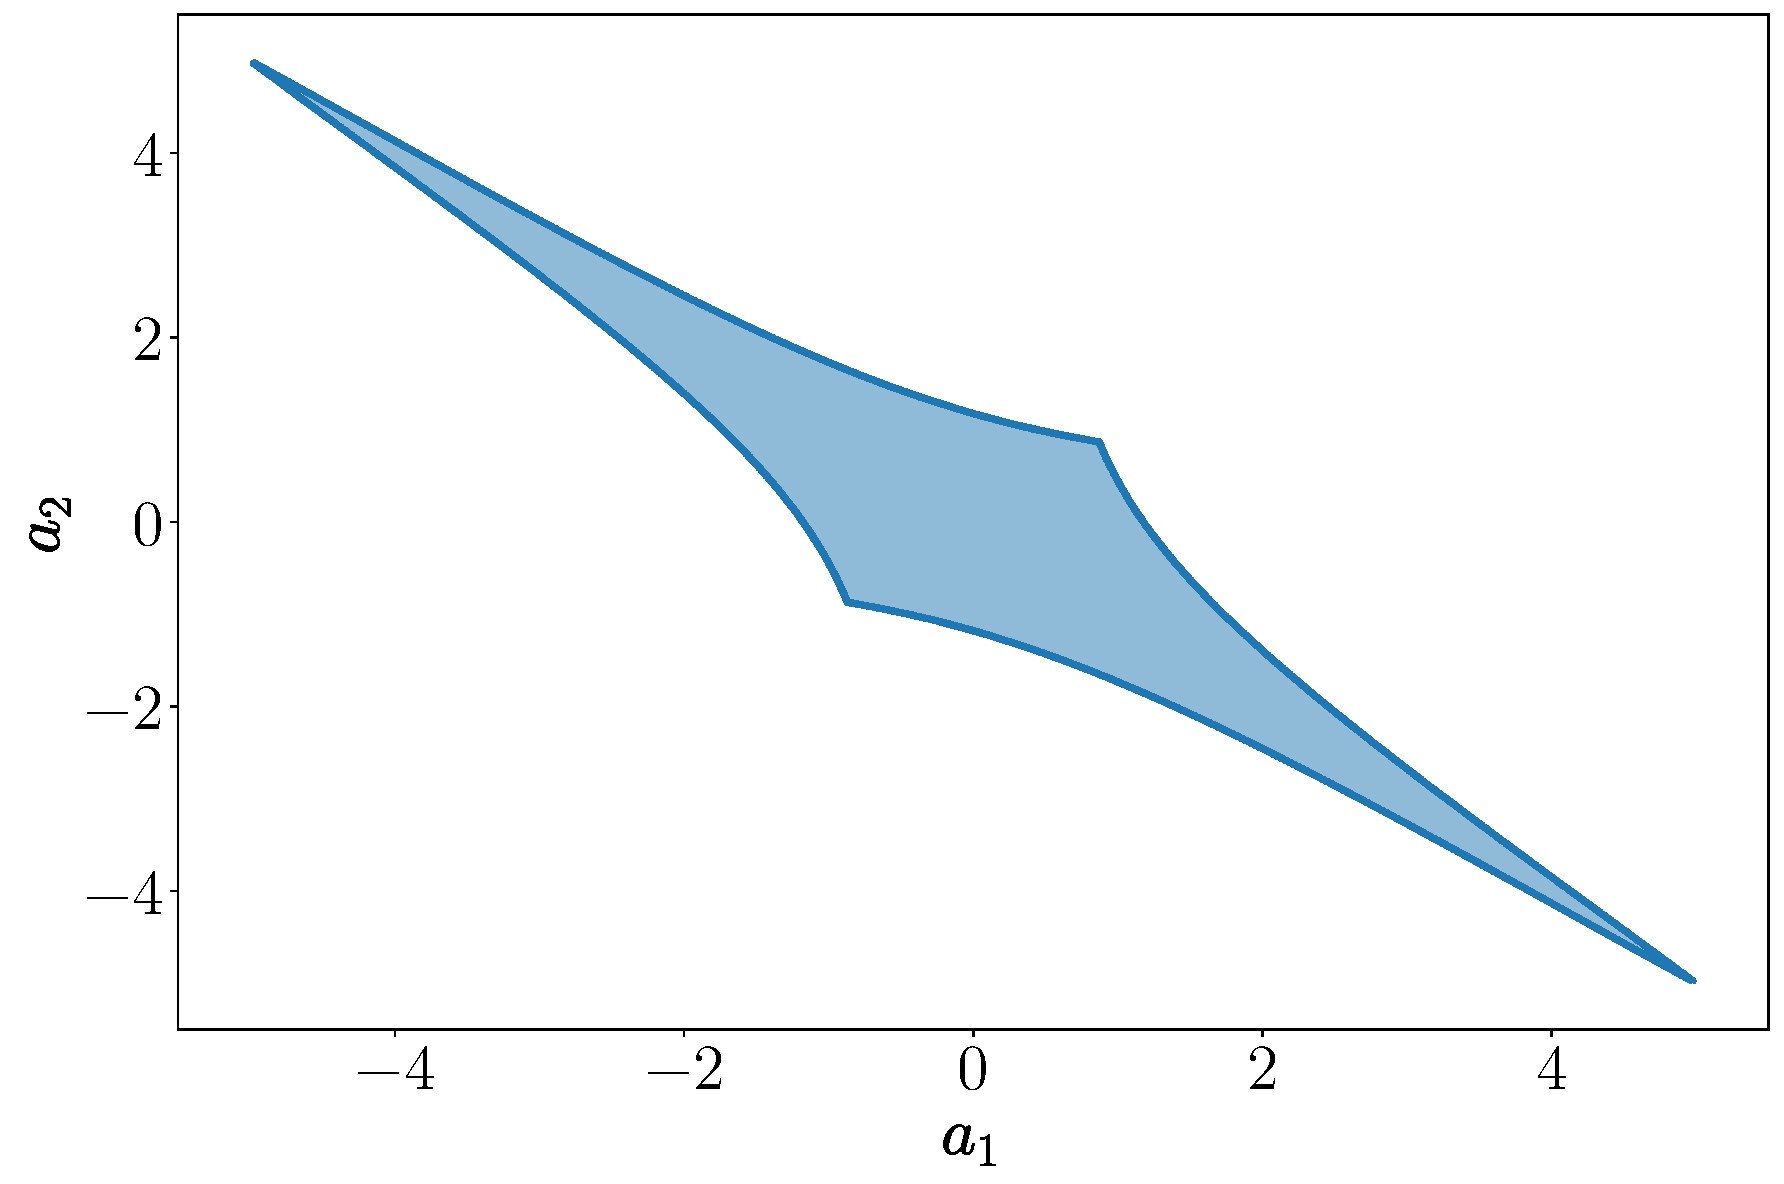
\includegraphics[scale = 0.15]{img/penrose_binaries/cmmr_par_region/par_region_b_0.98_q_1.0.pdf}
    \label{ch:penrose_binaries/fig:par_reg_i}
  }
  \caption{Parameter space variations in the CMMR solution. All $a_1$ and $a_2$ values inside of the blue region represent a valid black hole binary solution for a set of indicated $q$ and $b$ values.}
  \label{ch:penrose_binaries/fig:parameter_space}
\end{figure}

\subsection{Ergospheres}

In the context of stationary space-times the ergosphere is defined as the region in which observers can no longer be static and are ``dragged'' along the space-time's rotation. More precisely it is the region in which the time translation Killing vector field $K = \partial_t$ becomes space-like, that is, $\mtrtens{\mu}{\nu}\tens{K}{\mu}{}\tens{K}{\nu}{} >0$~\cite{carroll}. In the specific case of the CMMR metric, by employing Eq.~\eqref{ch:penrose_binaries/eq:line_element} we see that the ergosphere is the locus of all points $(\rho,z)$ that satisfy
%
\begin{equation}
  f(\rho,z) < 0.
  \label{ch:penrose_binaries/eq:ergosphere_def}
\end{equation}

Given the complexity of $f(\rho,z)$ it is extremely difficult (or even impossible) to find an explicit expression for $\rho$ and $z$ that satisfy Eq.~\eqref{ch:penrose_binaries/eq:ergosphere_def} thus we will visualize the ergospheres and their features in the CMMR solution numerically. Knowing that the relation between Weyl's radial coordinate $\rho$ and Cartesian coordinates $x$ and $y$ are $x = \rho\cos\varphi$ and $y = \rho\sin\varphi$ we can project and plot $f(\rho,z)$ in the $x$-$z$ plane by choosing $\varphi=0$.

To create the plots, we have fixed $q = 1.0$ and $|a_{1,2}| = 0.65$ while gradually increased $b$ from $0.3$ to $0.98$. This allows us to view the ergosphere around each constituent of the binary changing as their mutual interaction grows stronger. In Fig.~\ref{ch:penrose_binaries/fig:ergo_equal_spin} we show the variation of the ergosphere for constituents of aligned spins and in Fig.~\ref{ch:penrose_binaries/fig:ergo_unequal_spin} for constituents with anti-aligned spins. In all of the figures the ergosphere is the light blue region, bounded by the darker blue line and the event horizons are black lines. In both cases, the ergospheres start localized around each black hole. The choice of parameters in the figures intentionally lead to horizons that are initially very short which means that the black hole are spinning close to extremality.

\begin{figure}
  \centering
  \subfloat[$b=0.3$]{
    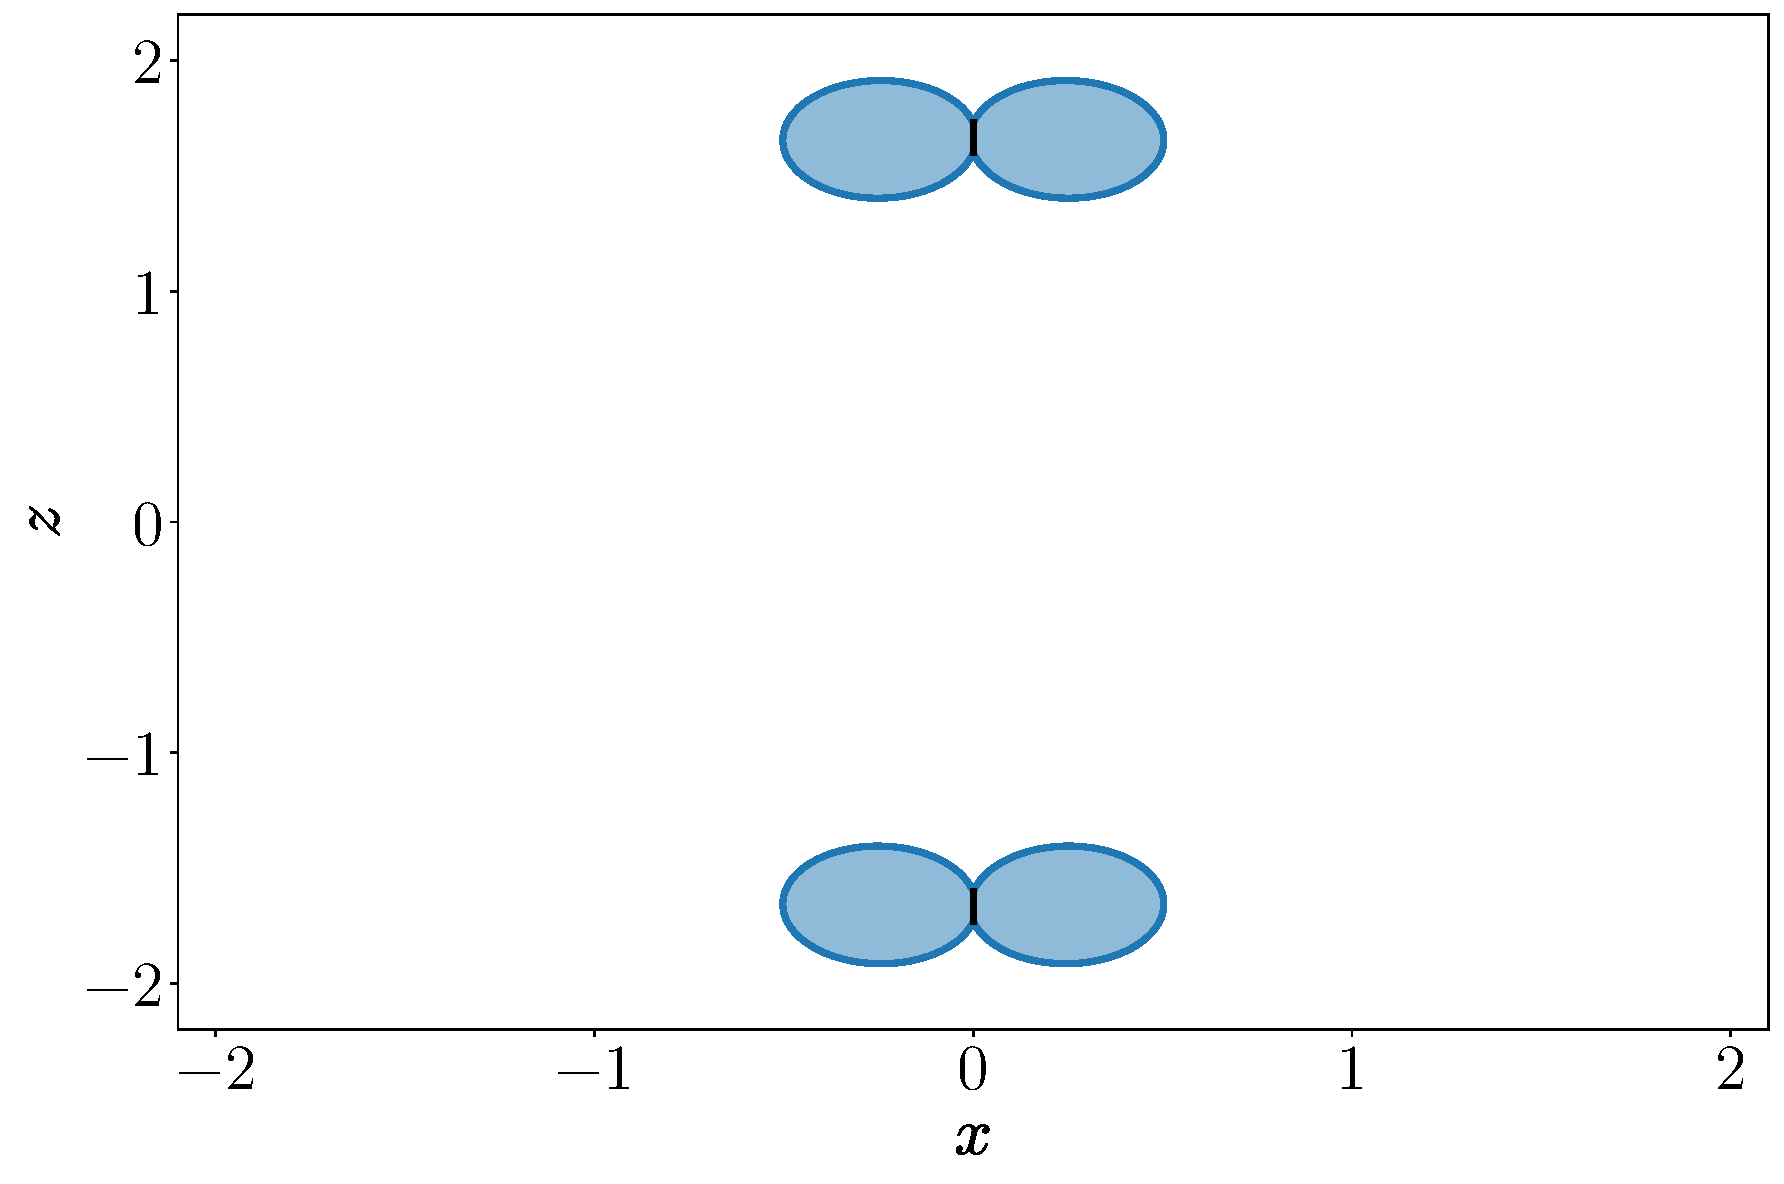
\includegraphics[scale = 0.22]{img/penrose_binaries/cmmr_ergo/ergo_b_0.3_q_1.0_a1_0.65_a2_0.65.pdf}
    \label{ch:penrose_binaries/fig:ergo_equal_a}
  }
  \subfloat[$b=0.5$]{
    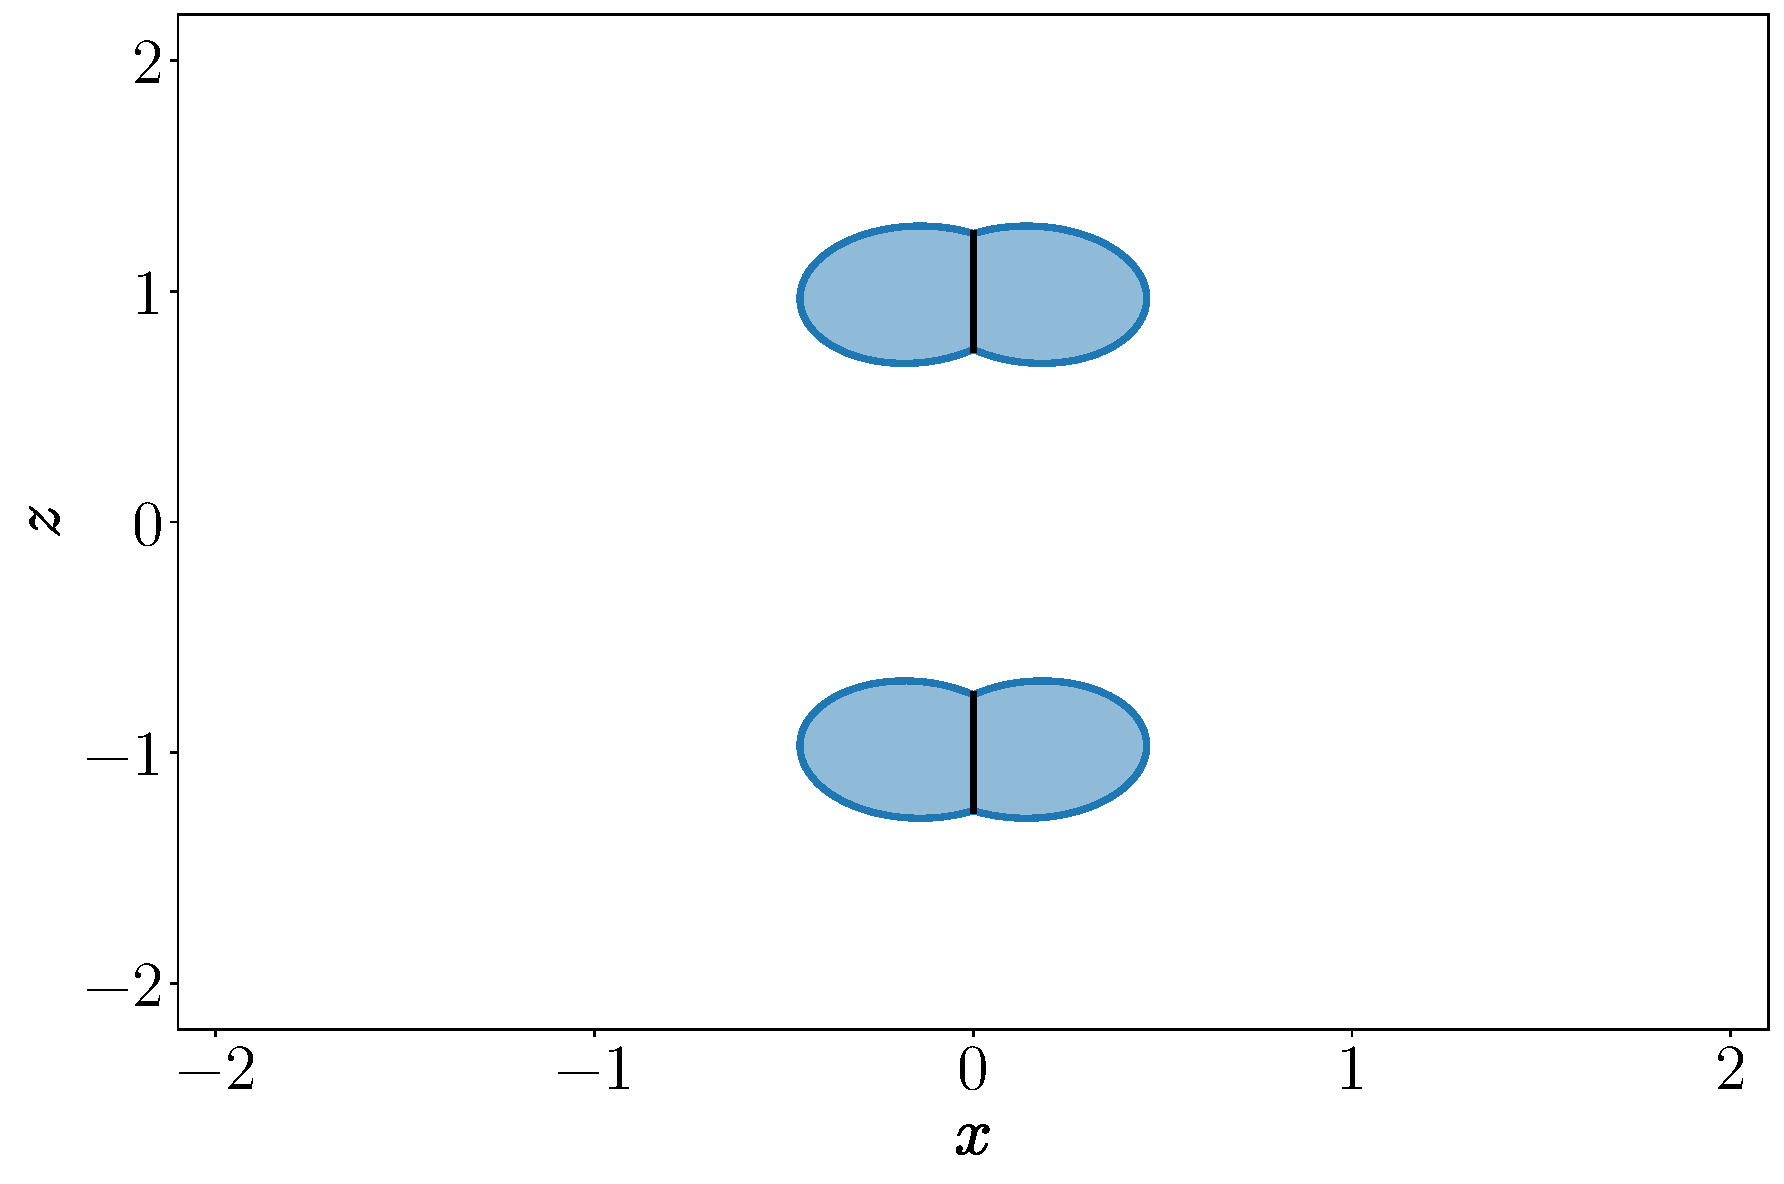
\includegraphics[scale = 0.22]{img/penrose_binaries/cmmr_ergo/ergo_b_0.5_q_1.0_a1_0.65_a2_0.65.pdf}
    \label{ch:penrose_binaries/fig:ergo_equal_b}
  }
  \newline
  \subfloat[$b=0.7$]{
    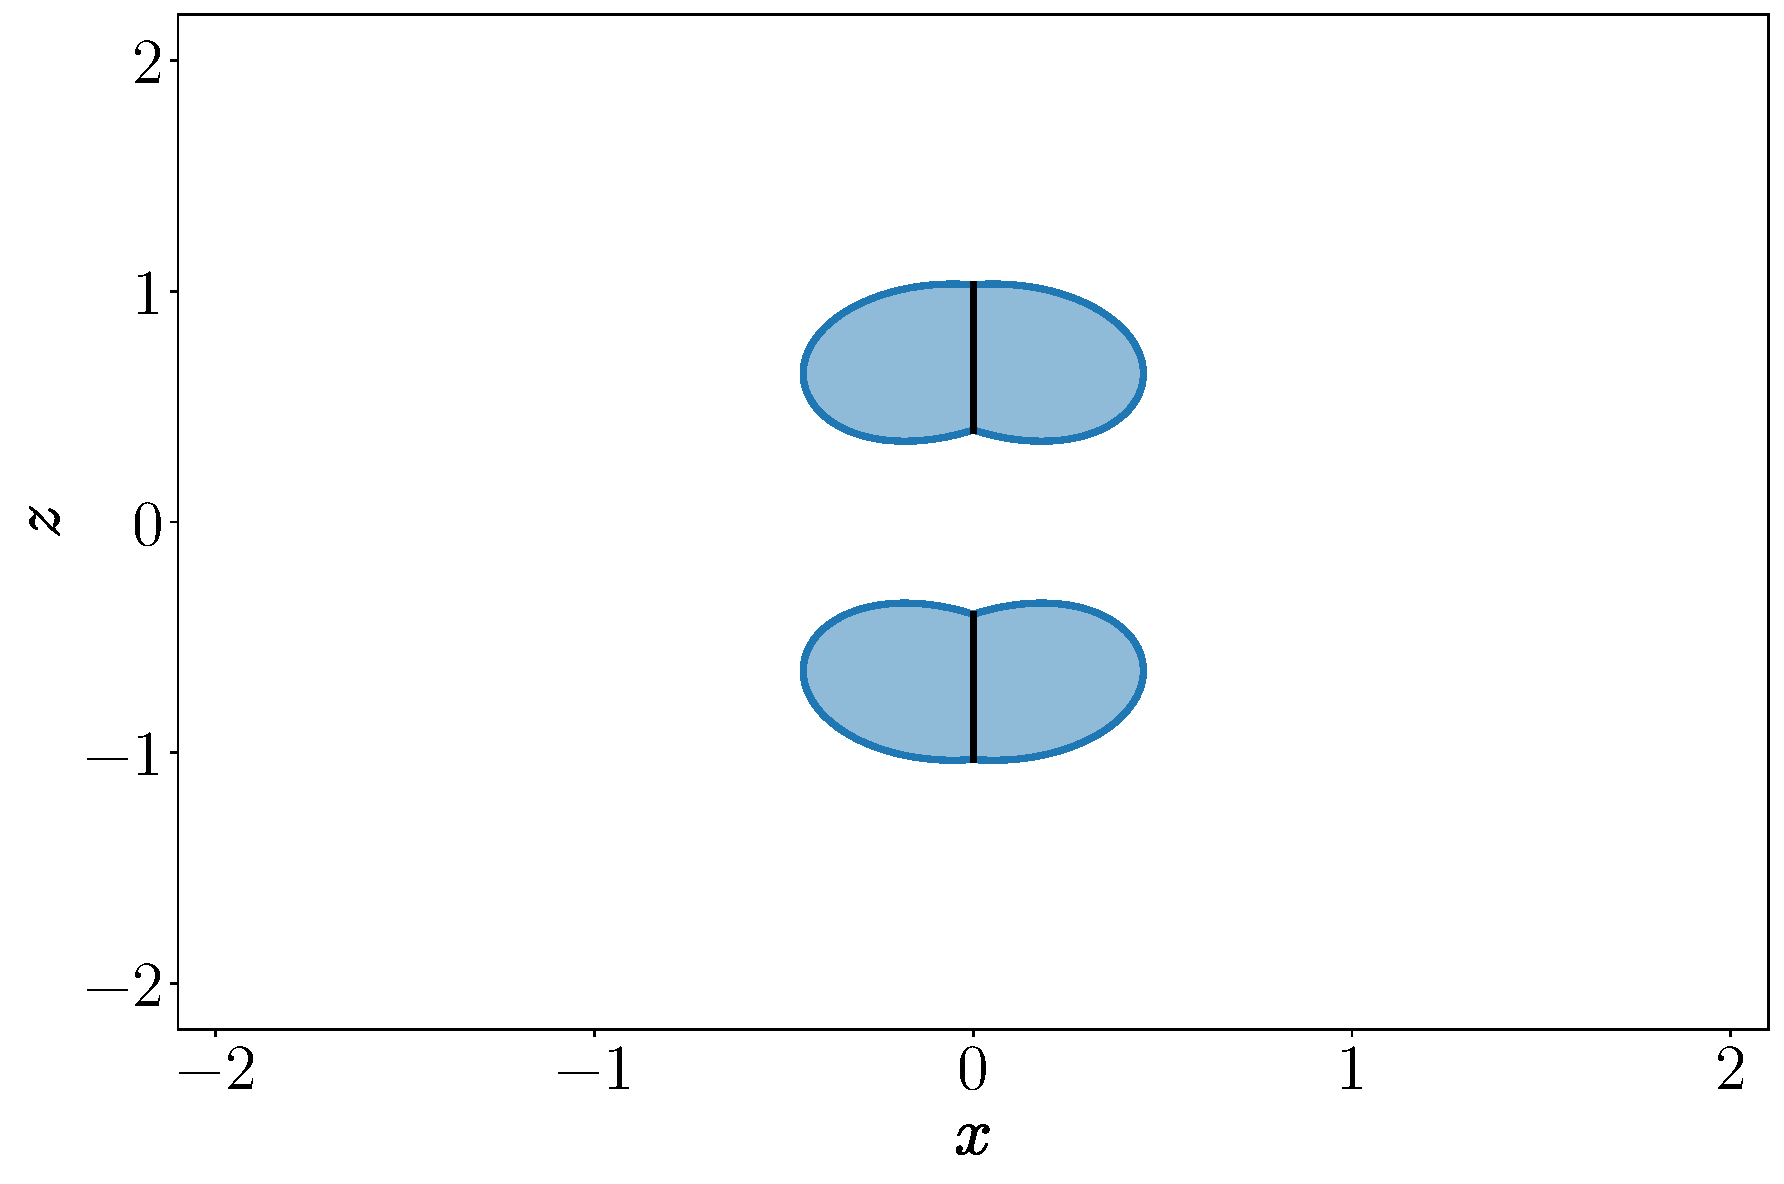
\includegraphics[scale = 0.22]{img/penrose_binaries/cmmr_ergo/ergo_b_0.7_q_1.0_a1_0.65_a2_0.65.pdf}
    \label{ch:penrose_binaries/fig:ergo_equal_c}
  }
  \subfloat[$b=0.98$]{
    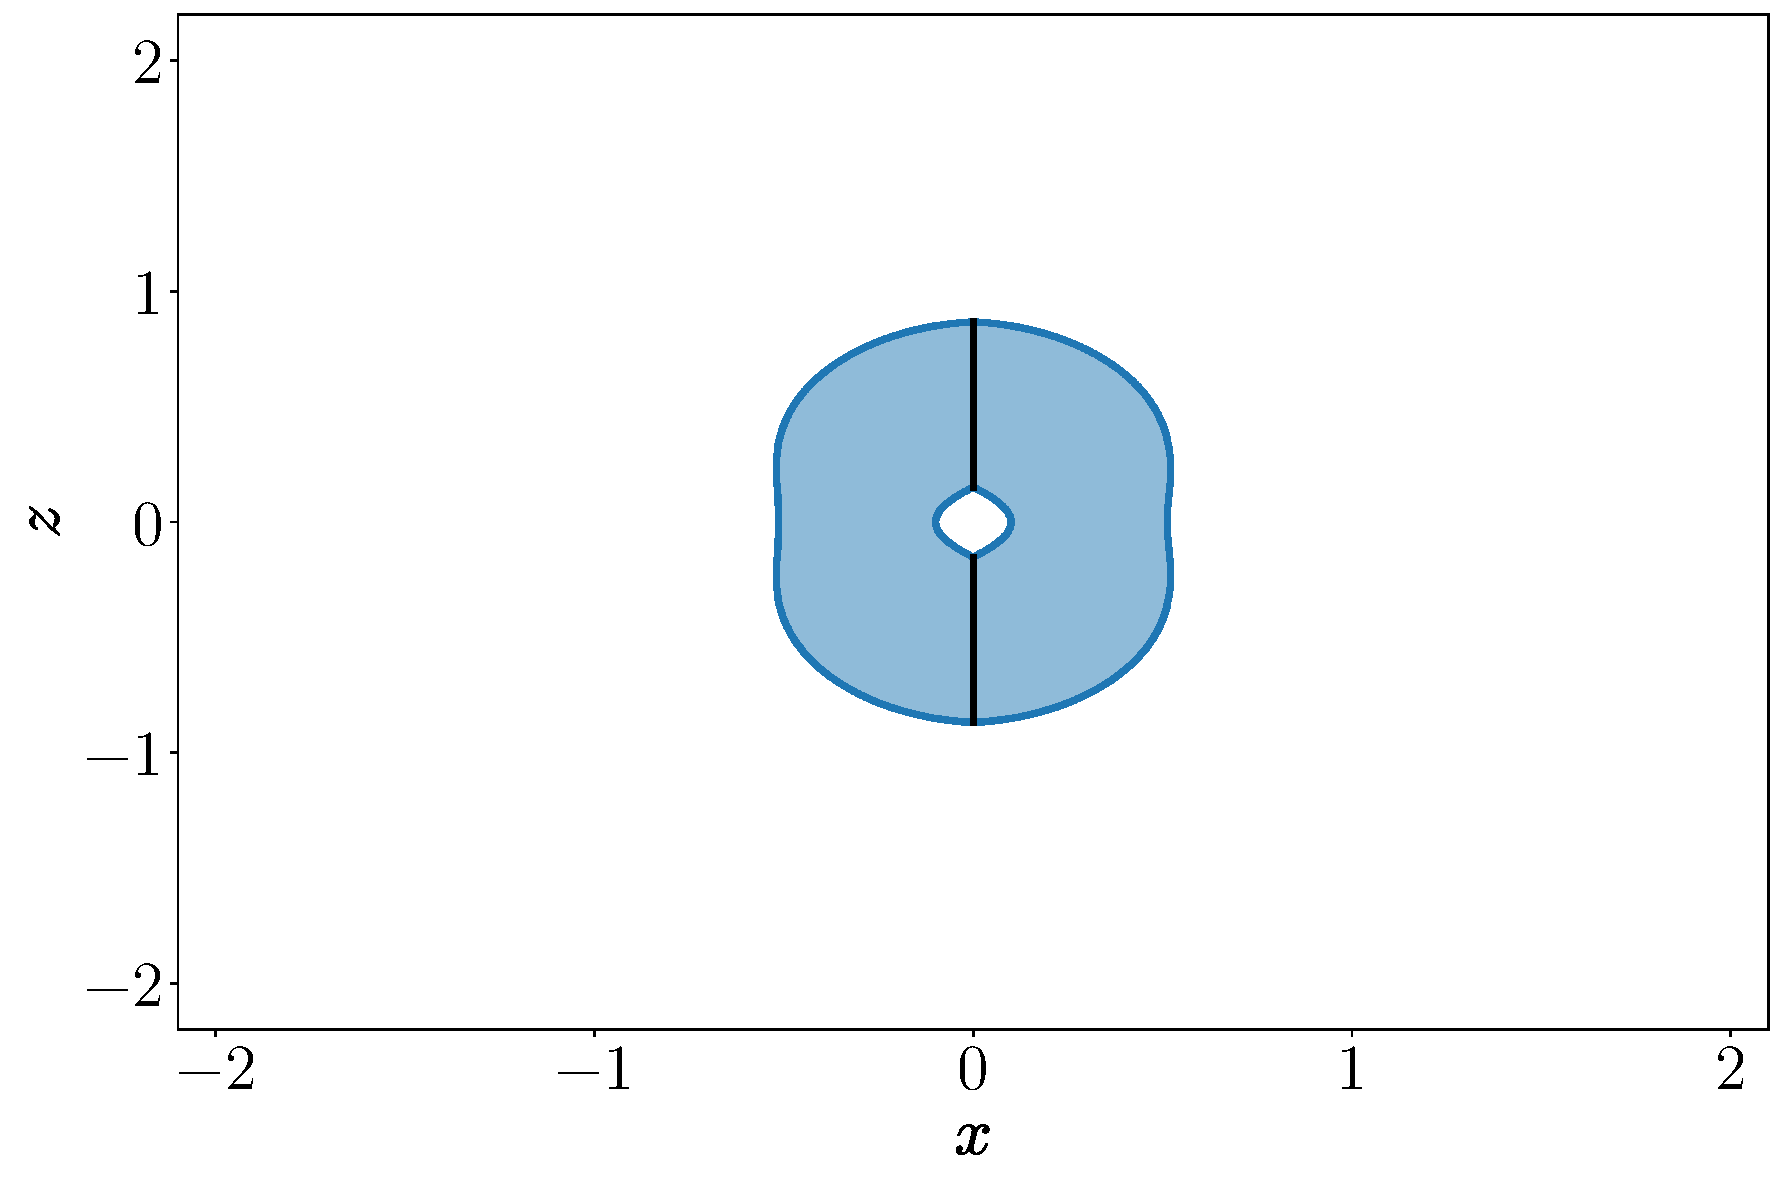
\includegraphics[scale = 0.22]{img/penrose_binaries/cmmr_ergo/ergo_b_0.98_q_1.0_a1_0.65_a2_0.65.pdf}
    \label{ch:penrose_binaries/fig:ergo_equal_d}
  }
  \caption{Ergosphere of a binary Kerr black hole system with mass ratio $q=1.0$ and aligned spins $a_1=0.65$ and $a_2=0.65$ for differente separation parameters. The blu region represents the ergosphere while the black lines represent the event horizons.}
  \label{ch:penrose_binaries/fig:ergo_equal_spin}
\end{figure}

\begin{figure}
  \centering
  \subfloat[$b=0.3$]{
    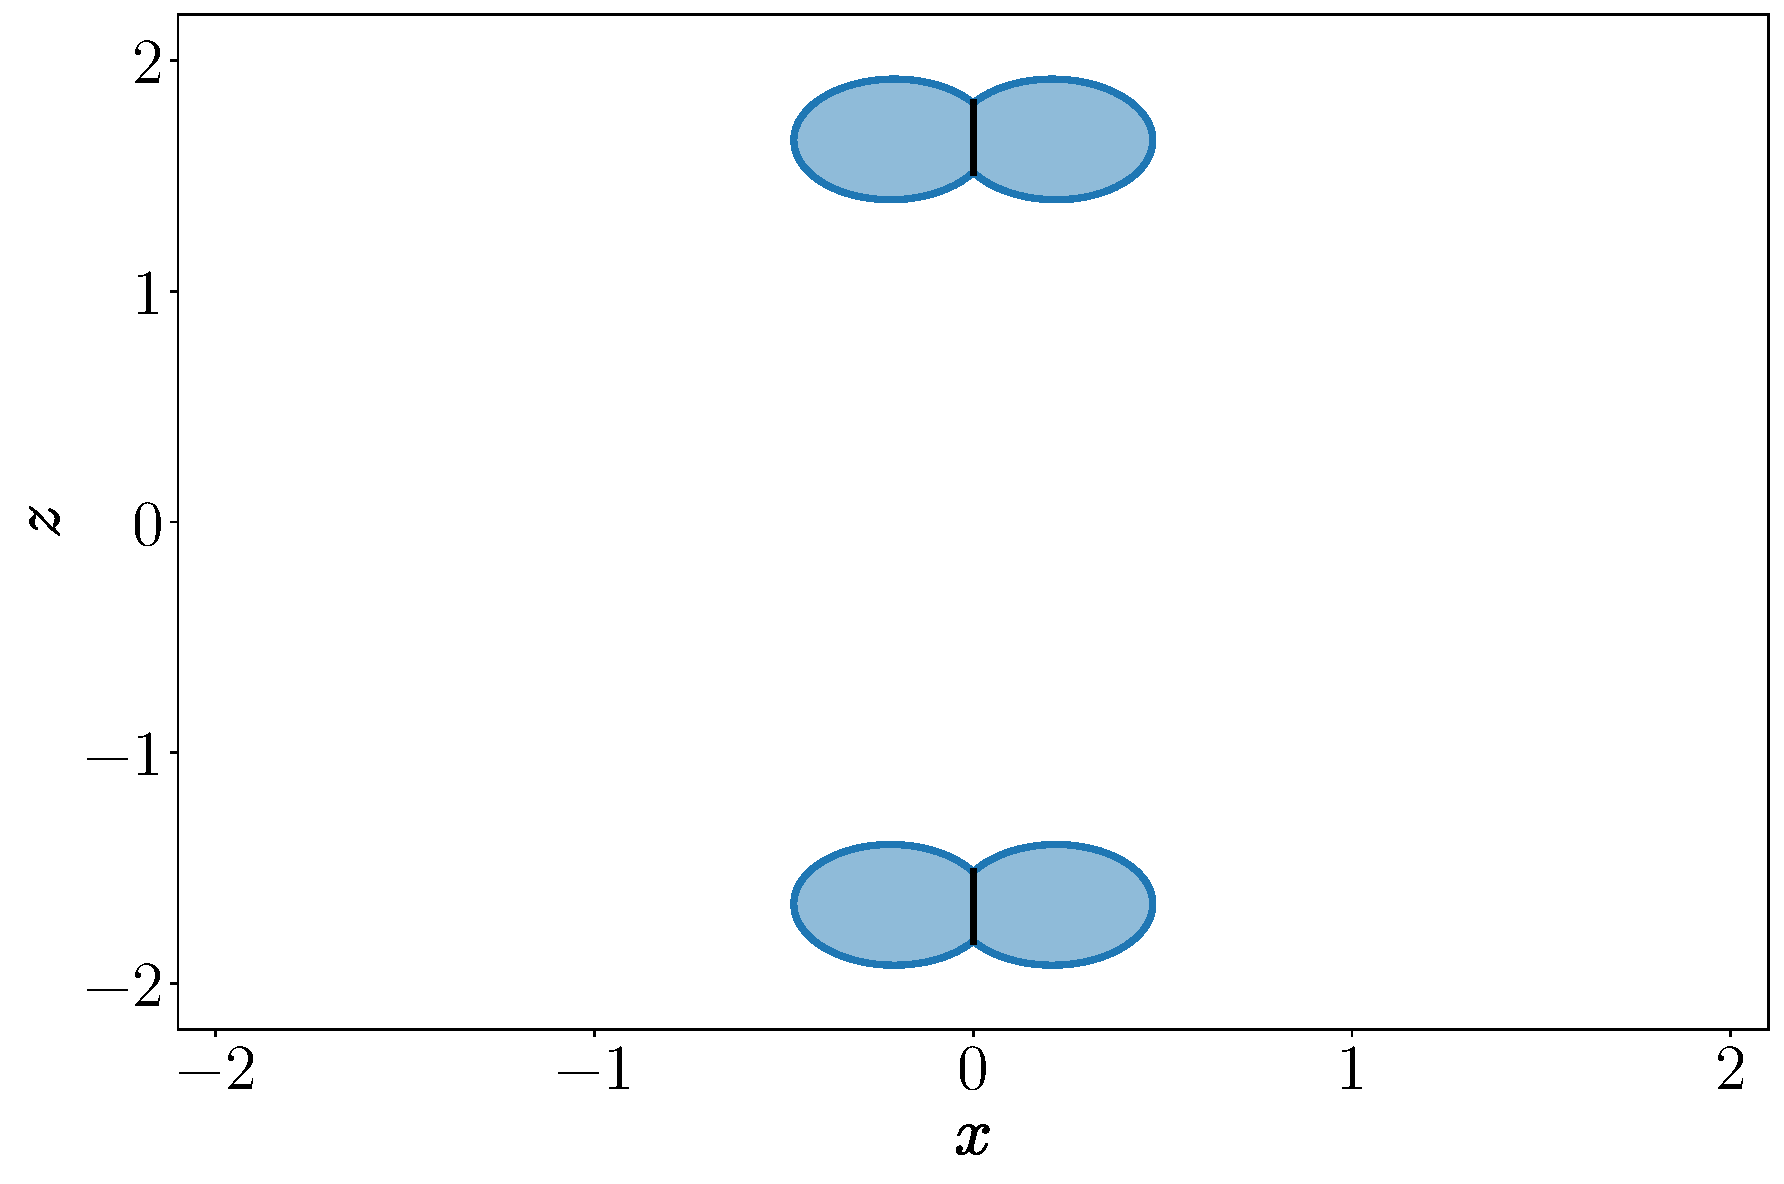
\includegraphics[scale = 0.22]{img/penrose_binaries/cmmr_ergo/ergo_b_0.3_q_1.0_a1_-0.65_a2_0.65.pdf}
    \label{ch:penrose_binaries/fig:ergo_unequal_a}
  }
  \subfloat[$b=0.5$]{
    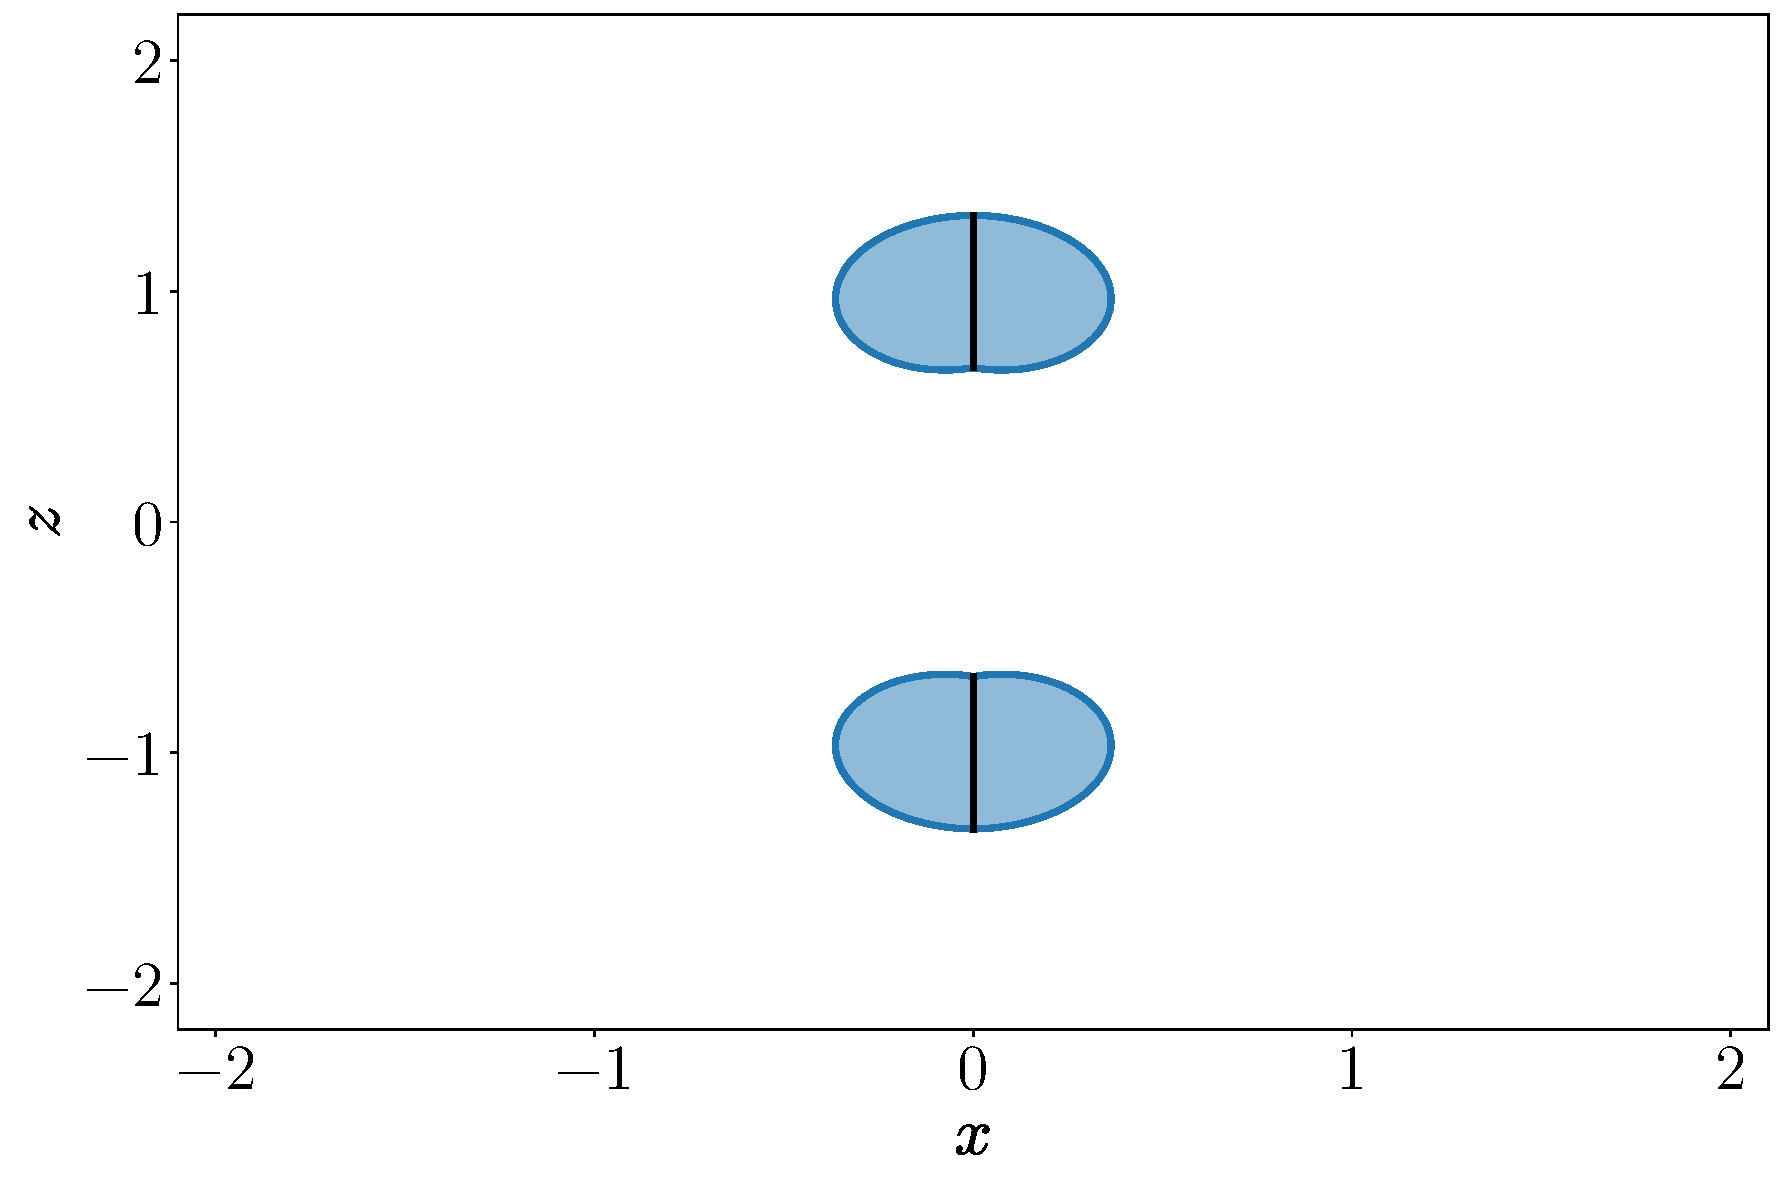
\includegraphics[scale = 0.22]{img/penrose_binaries/cmmr_ergo/ergo_b_0.5_q_1.0_a1_-0.65_a2_0.65.pdf}
    \label{ch:penrose_binaries/fig:ergo_unequal_b}
  }
  \newline
  \subfloat[$b=0.7$]{
    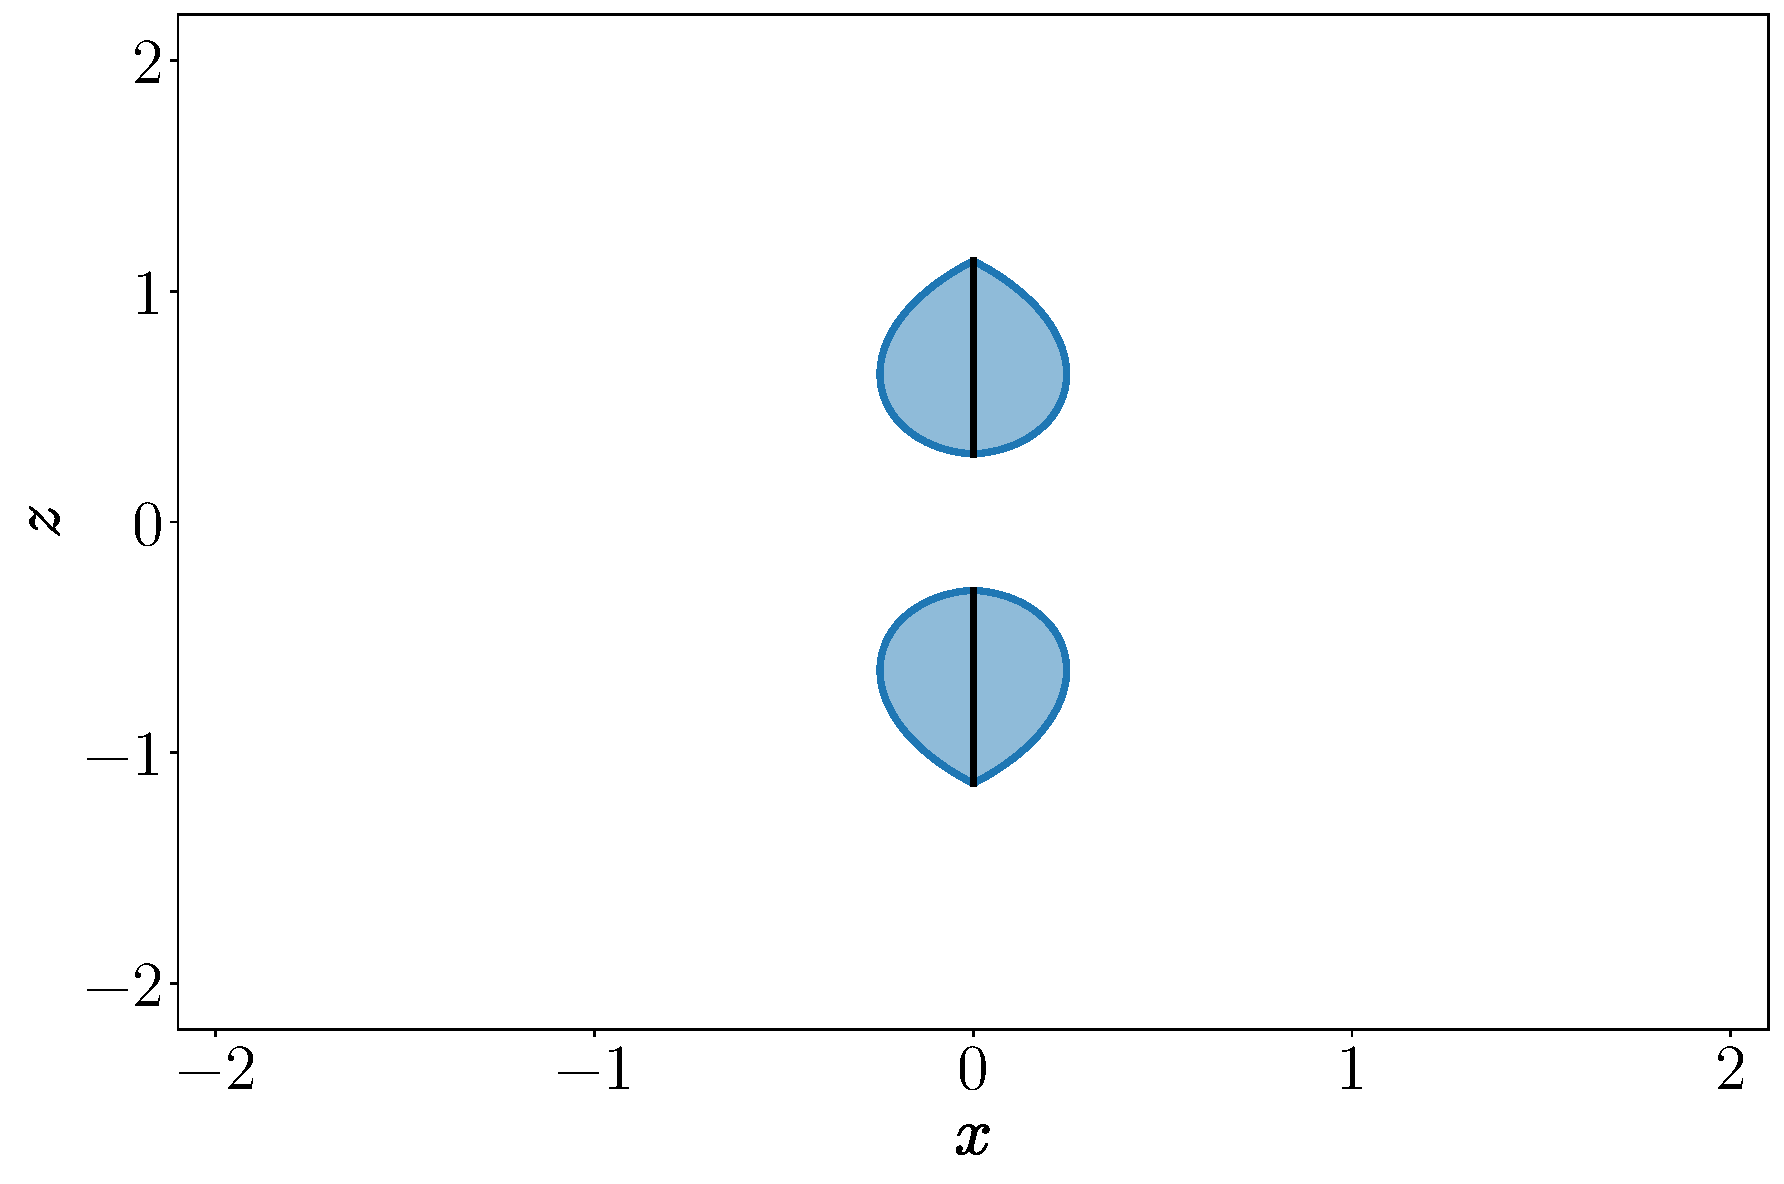
\includegraphics[scale = 0.22]{img/penrose_binaries/cmmr_ergo/ergo_b_0.7_q_1.0_a1_-0.65_a2_0.65.pdf}
    \label{ch:penrose_binaries/fig:ergo_unequal_c}
  }
  \subfloat[$b=0.98$]{
    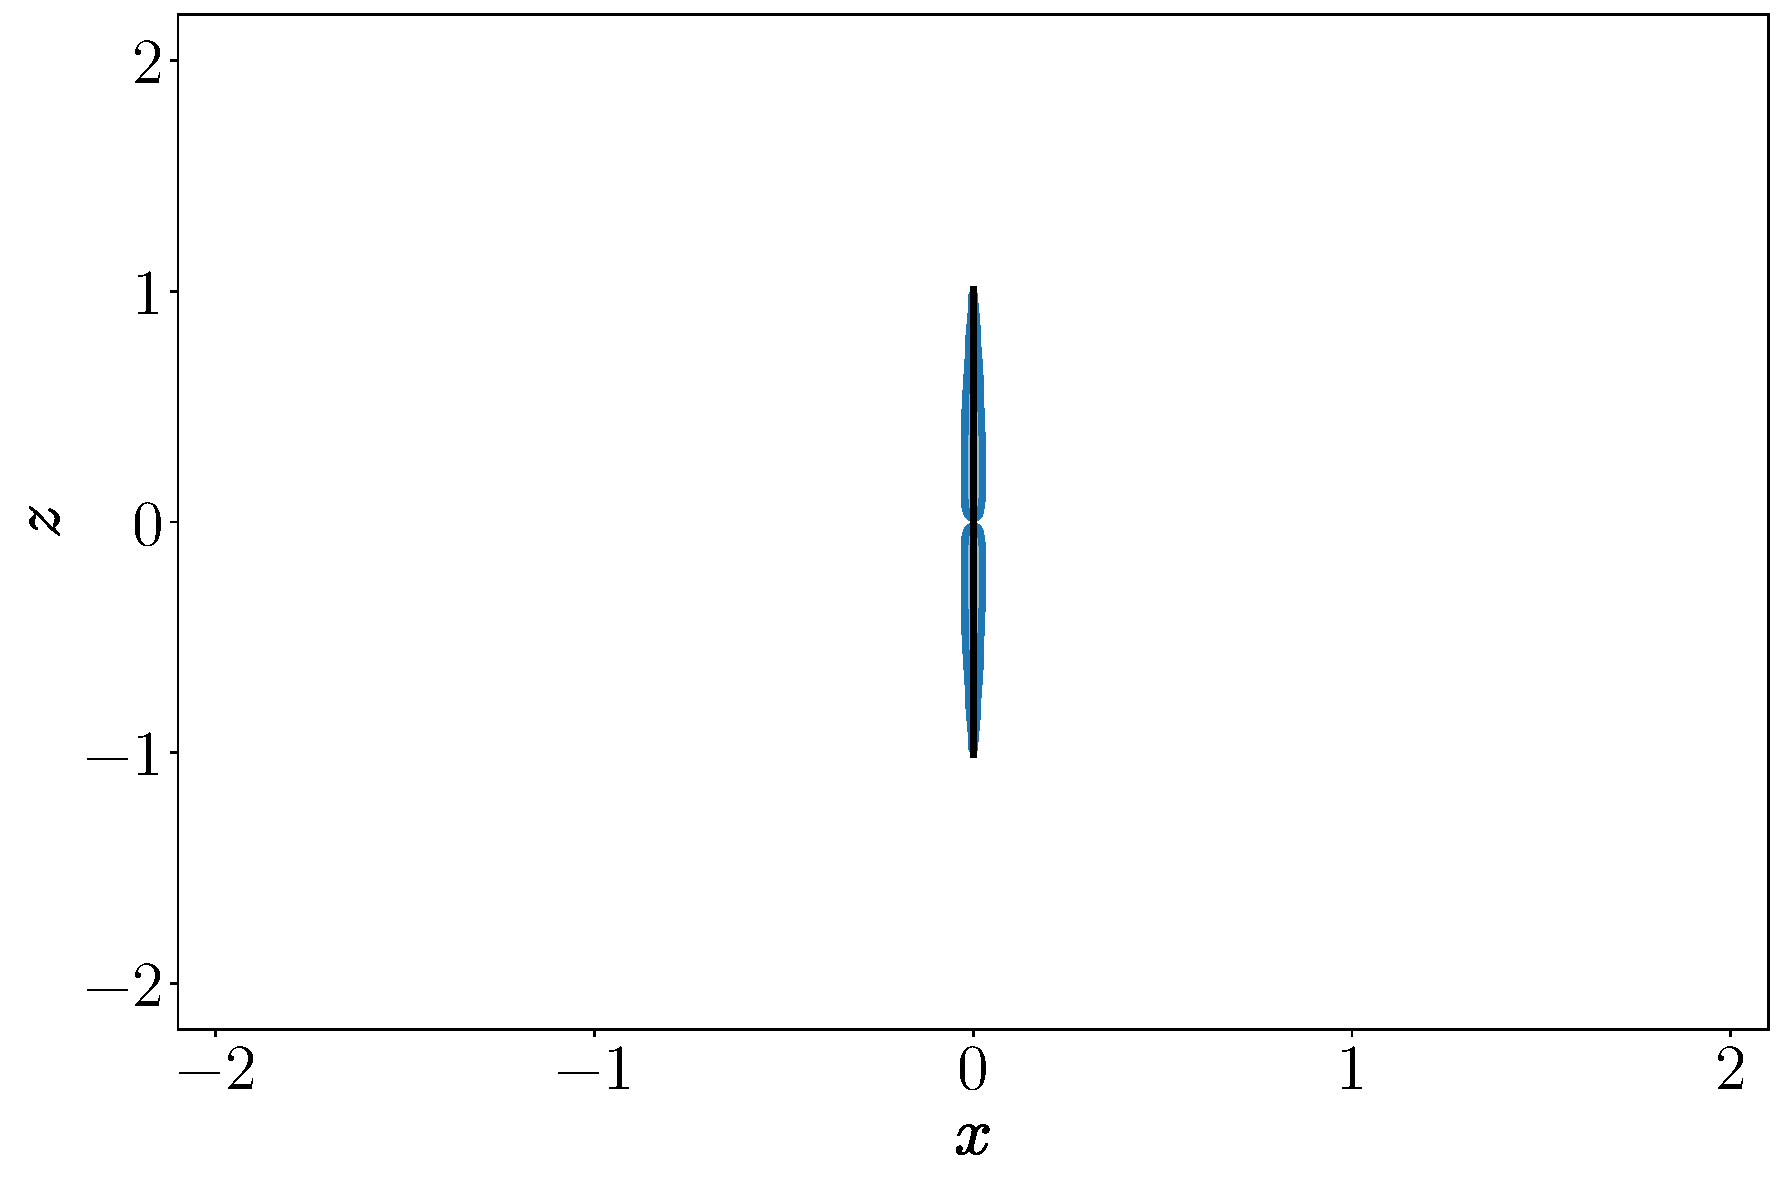
\includegraphics[scale = 0.22]{img/penrose_binaries/cmmr_ergo/ergo_b_0.98_q_1.0_a1_-0.65_a2_0.65}
    \label{ch:penrose_binaries/fig:ergo_unequal_d}
  }
  \caption{Ergosphere of a binary Kerr black hole system with mass ratio $q=1.0$ and aligned spins $a_1=0.65$ and $a_2=0.65$ for differente separation parameters. The blu region represents the ergosphere while the black lines represent the event horizons.}
  \label{ch:penrose_binaries/fig:ergo_unequal_spin}
\end{figure}

Let us now focus on Fig.~\ref{ch:penrose_binaries/fig:ergo_equal_spin}. As the holes get closer, the familiar ``infinity shaped'' ergosphere around each hole starts to deform in a very particular way: both of the tips of each ergosphere start to bend towards the other until they touch and eventually form a larger region that encompasses both holes and. Even more interesting, as the system gets closer to merging, the event horizons themselves get ``stretched'' along the $z$ direction. It becomes clear that in this case the ergospheres and event horizons ``add up'' to create structures larger than the originals.

Switching focus to Fig.~\ref{ch:penrose_binaries/fig:ergo_unequal_spin} that in spite of the fact that the event horizons still ``stretch'' what appears to be the opposite of the aligned spin case happens for the ergospheres. Instead of bending towards each other they are repelled to the point that when they are close to merging, their shape becomes very thin and elongated. In other words, the ergospheres become \textit{spaghettifyied} and ``cancel out'' in the case of equal but anti-aligned spins.

These results are not physically surprising. One expects that black holes that have exactly the same spin but in opposite directions when merged create a resulting black hole that has more mass but no spin, that is, their counter rotation balances and cancels out. The opposite is expected to happen for black holes with aligned spins: both their masses and angular momenta are added up upon merging. The novelty of our work is, we believe, in the fact that even using an analytic solution containing an unphysical strut that keeps the black holes from colliding such features are apparent and can be demonstrated with relative ease.

Now that the general shapes and features of the ergospheres have been established, we can ask ourselves how far appart should the Kerr black holes be so that their individual ergospheres merge into one? From Fig.~\ref{ch:penrose_binaries/fig:ergo_unequal_spin} we can see that if the spins are exactly equal in modulus but differ in sign such merging is impossible. Nevertheless, from Fig.~\ref{ch:penrose_binaries/fig:ergo_equal_spin} we see that when the spins are equal we can be sure that such merging occurs for some value of $b$. It is not unreasonable to imagine that in the intermediary case is considered, that is anti-aligned spins that are not exactly equal, such merging also occurs.

In order to visualize the parameter regions that are able to produce connected ergospheres we plot the regions for which the parameters produce physical black hole binarys (i.e., black holes and not naked singularities) and $f(\rho,0) = 0$ for some value of $\rho$. These are the blue regions shown in Fig.~\ref{ch:penrose_binaries/fig:ergo_joined} where we increased $b$ from $0.89$ to $0.98$ while also increasing the mass ratio from $0.1$ to $1.0$ and in Fig.~\ref{ch:penrose_binaries/fig:ergo_joined_2} where $a_1$ and $q$ where fixed but $a_2$ and $b$ were allowed to change instead. It is extremely important to point out that despite what the figures indicate the configuration $a_1=a_2=0$ does not produce an ergosphere. These points are included in our graphs but should be disregarded as the CMMR solution in the form presented in Ref.~\cite{MANKO2020} (which is the source of all metric quantities used in this work) does not describe the black hole system correctly if one of the spins is zero. This case must be treated separately and is discussed in detail in Ref.~\cite{MANKO2019}.

Let us now focus on Fig.~\ref{ch:penrose_binaries/fig:ergo_joined}. For any given mass ratio, it is apparent that the increase in the distance parameter increases the overall size of the parameter region producing joint ergospheres. The most interesting feature is that certain configurations of equal but opposite spins can also produce a joined ergosphere if the masses are not equal. This can be easily seen in Fig.~\ref{ch:penrose_binaries/fig:ergo_joined_e} if $a_1=0.5$ and $a_2=-0.5$.

In Fig.~\ref{ch:penrose_binaries/fig:ergo_joined_2} we look at the influence of the distance parameter in more detail. The first apparent feature is that for equal mass binaries, the configuration where $a_2=-a_1$ never produces a joined ergosphere, even for very large distance parameters (and thus very small distances). This can easily be seen in Fig.~\ref{ch:penrose_binaries/fig:ergo_joined_2_b} and Fig.~\ref{ch:penrose_binaries/fig:ergo_joined_2_d}. We can also observe that for a fixed mas ratio, an increase in the fixed spin parameter $a_1$ causes the area of the graph to become larger in the negative region of $a_2$ which can be seen in Fig.~\ref{ch:penrose_binaries/fig:ergo_joined_2_a} and Fig.~\ref{ch:penrose_binaries/fig:ergo_joined_2_c}. This indicates that for binaries with unequal masses, configurations with opposite spins can generate joined ergospheres more easily. Furthermore we can observe the universal need of $b$ being large in order to create joined ergospheres.

\begin{figure}
  \centering
  \subfloat[$b=0.89$, $q=0.1$]{
    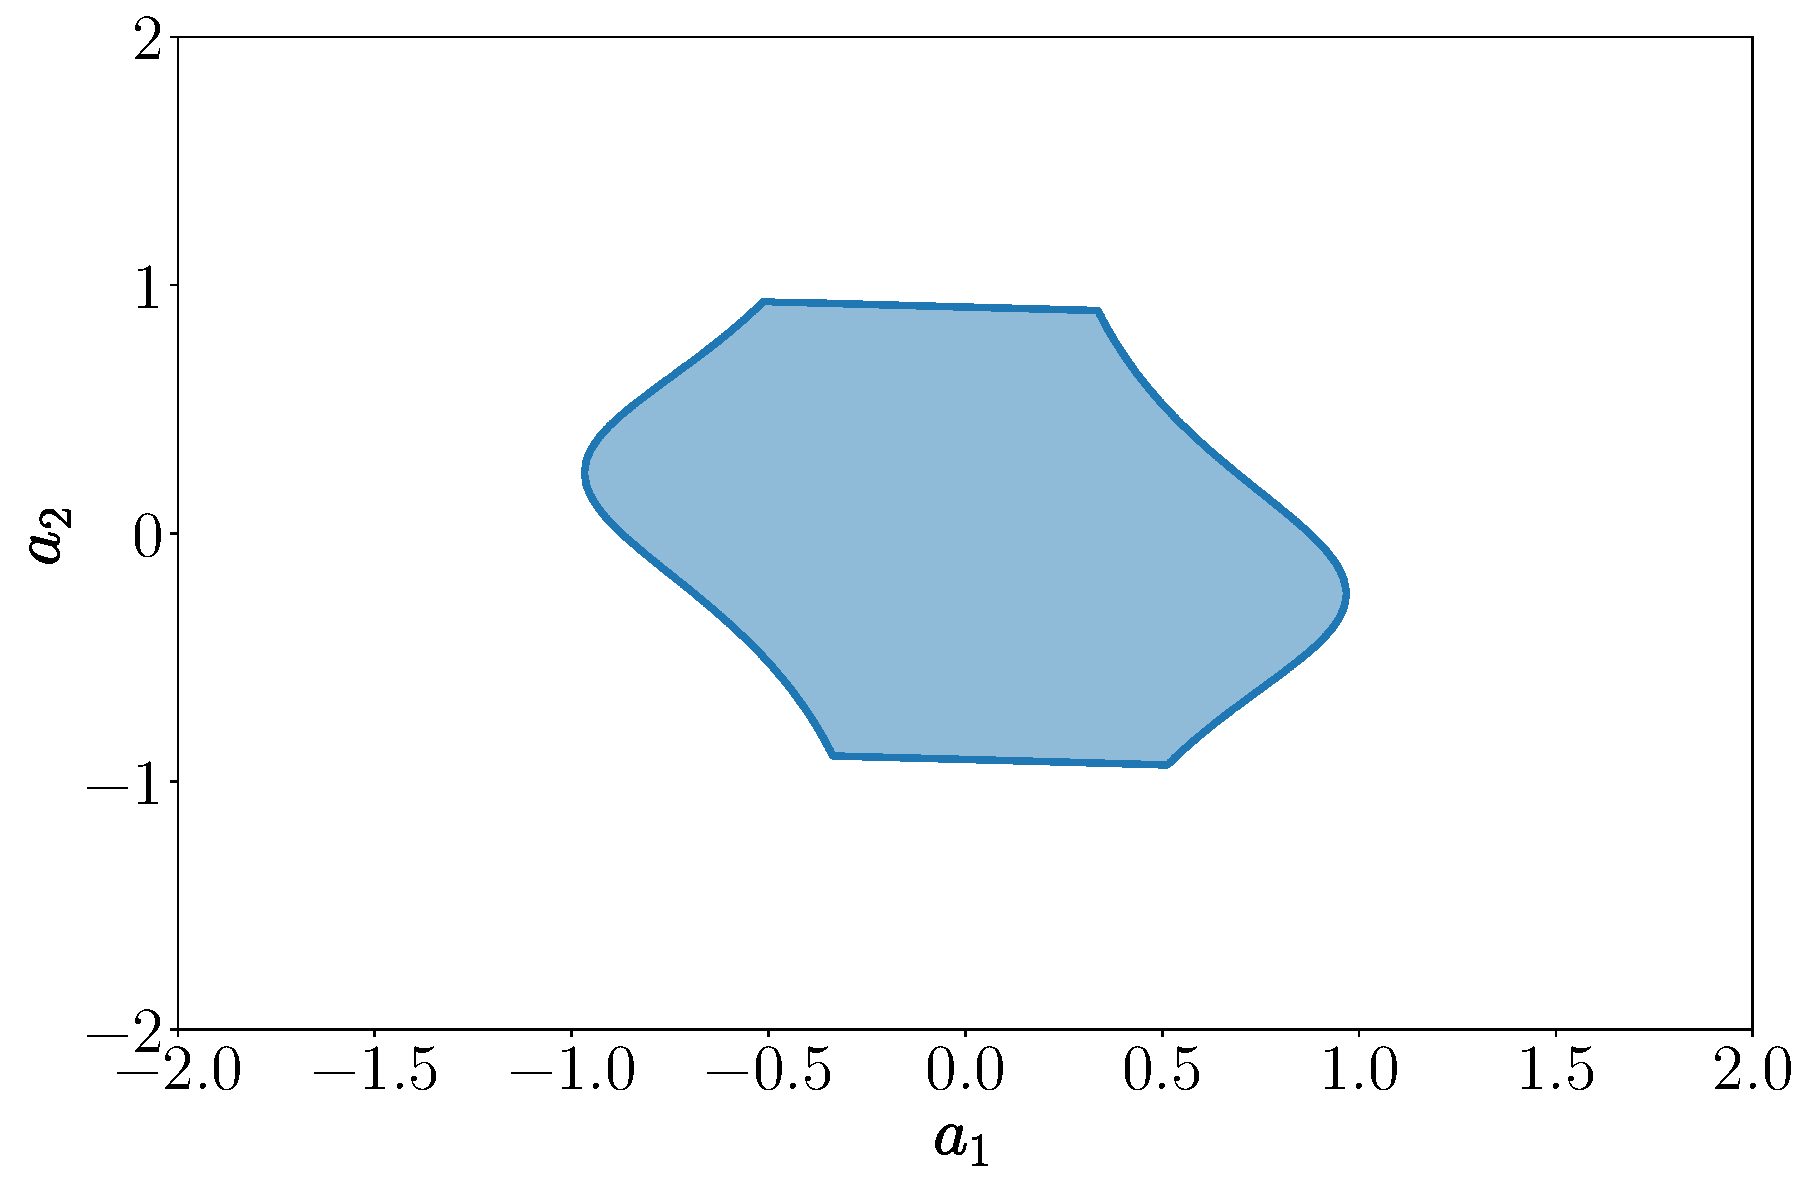
\includegraphics[scale = 0.15]{img/penrose_binaries/cmmr_joined_ergo/joined_ergo_b_0.89_q_0.1}
    \label{ch:penrose_binaries/fig:ergo_joined_a}
  }
  \subfloat[$b=0.89$, $q=0.5$]{
    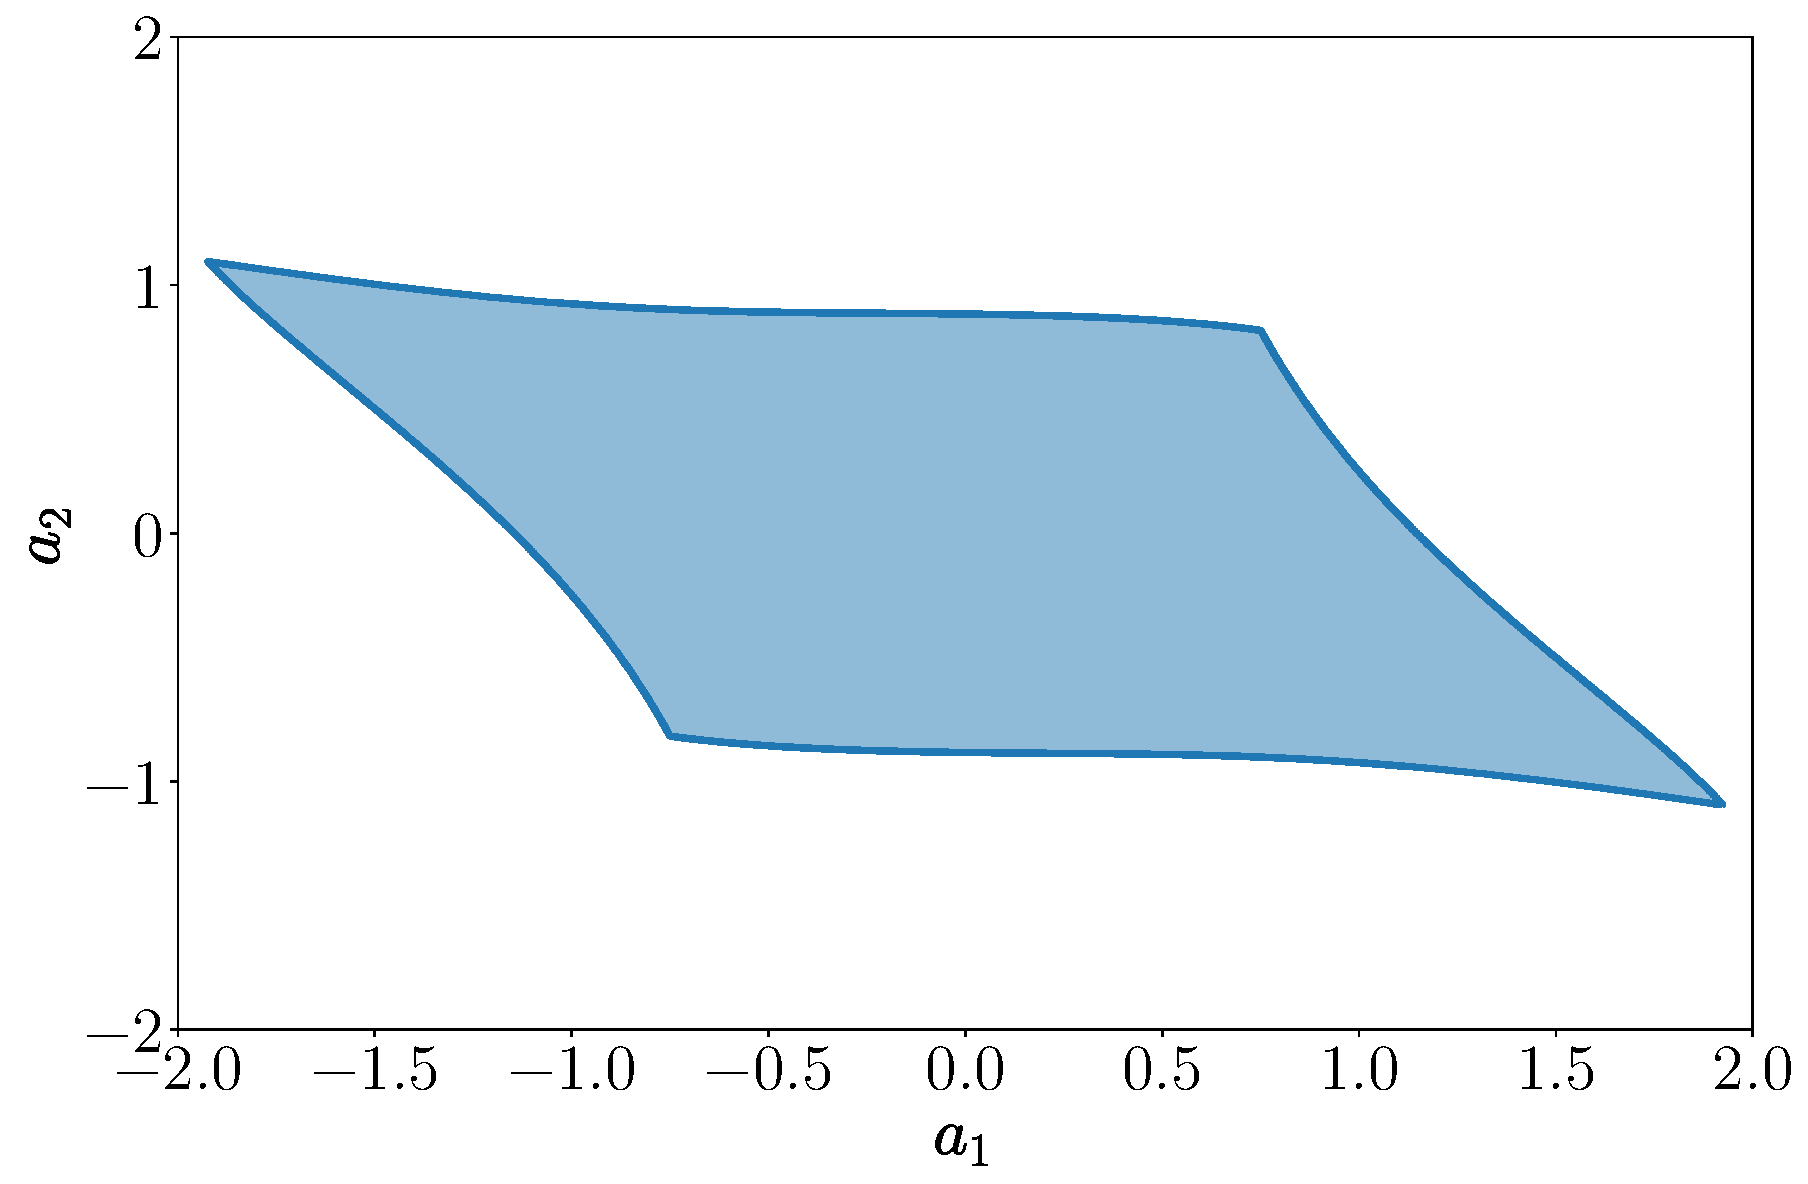
\includegraphics[scale = 0.15]{img/penrose_binaries/cmmr_joined_ergo/joined_ergo_b_0.89_q_0.5}
    \label{ch:penrose_binaries/fig:ergo_joined_b}
  }
  \subfloat[$b=0.89$, $q=1.0$]{
    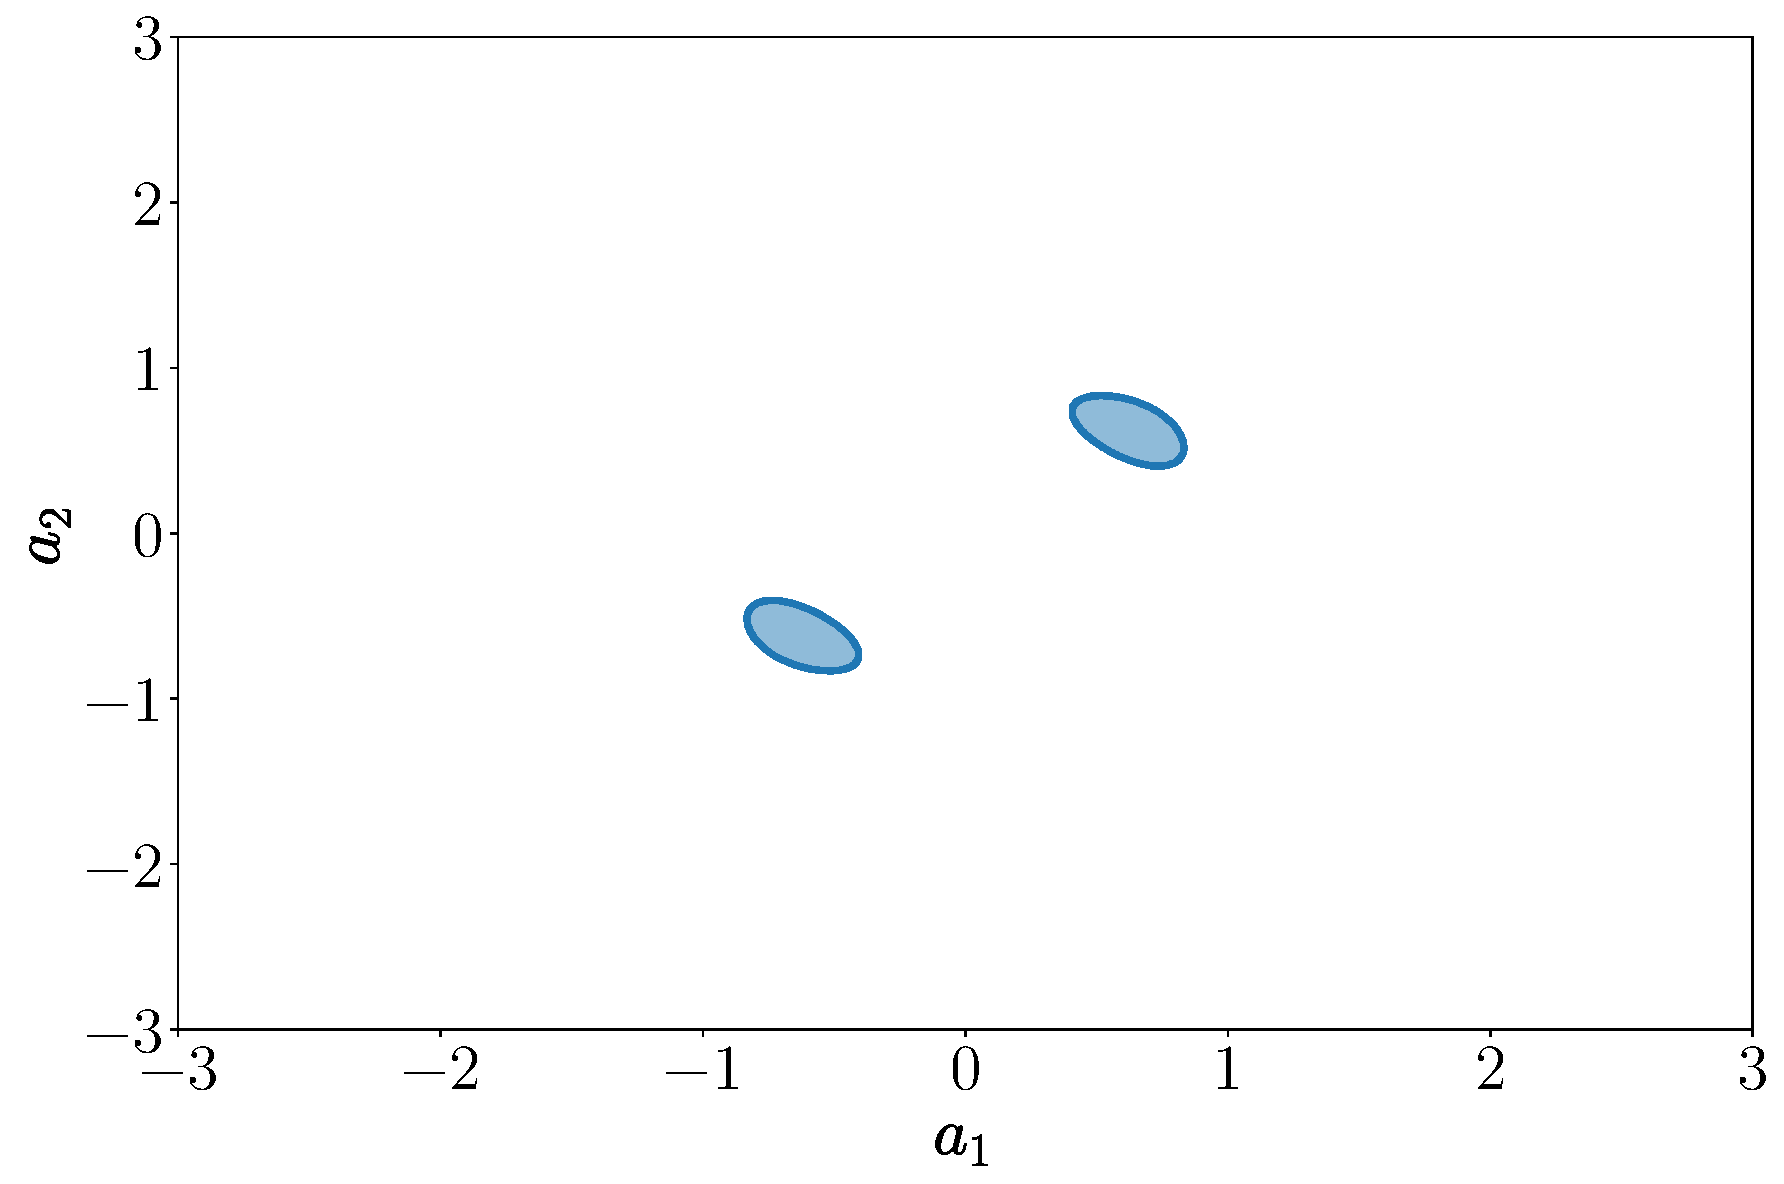
\includegraphics[scale = 0.15]{img/penrose_binaries/cmmr_joined_ergo/joined_ergo_b_0.89_q_1.0}
    \label{ch:penrose_binaries/fig:ergo_joined_c}
  }
  \newline
  \subfloat[$b=0.93$, $q=0.1$]{
    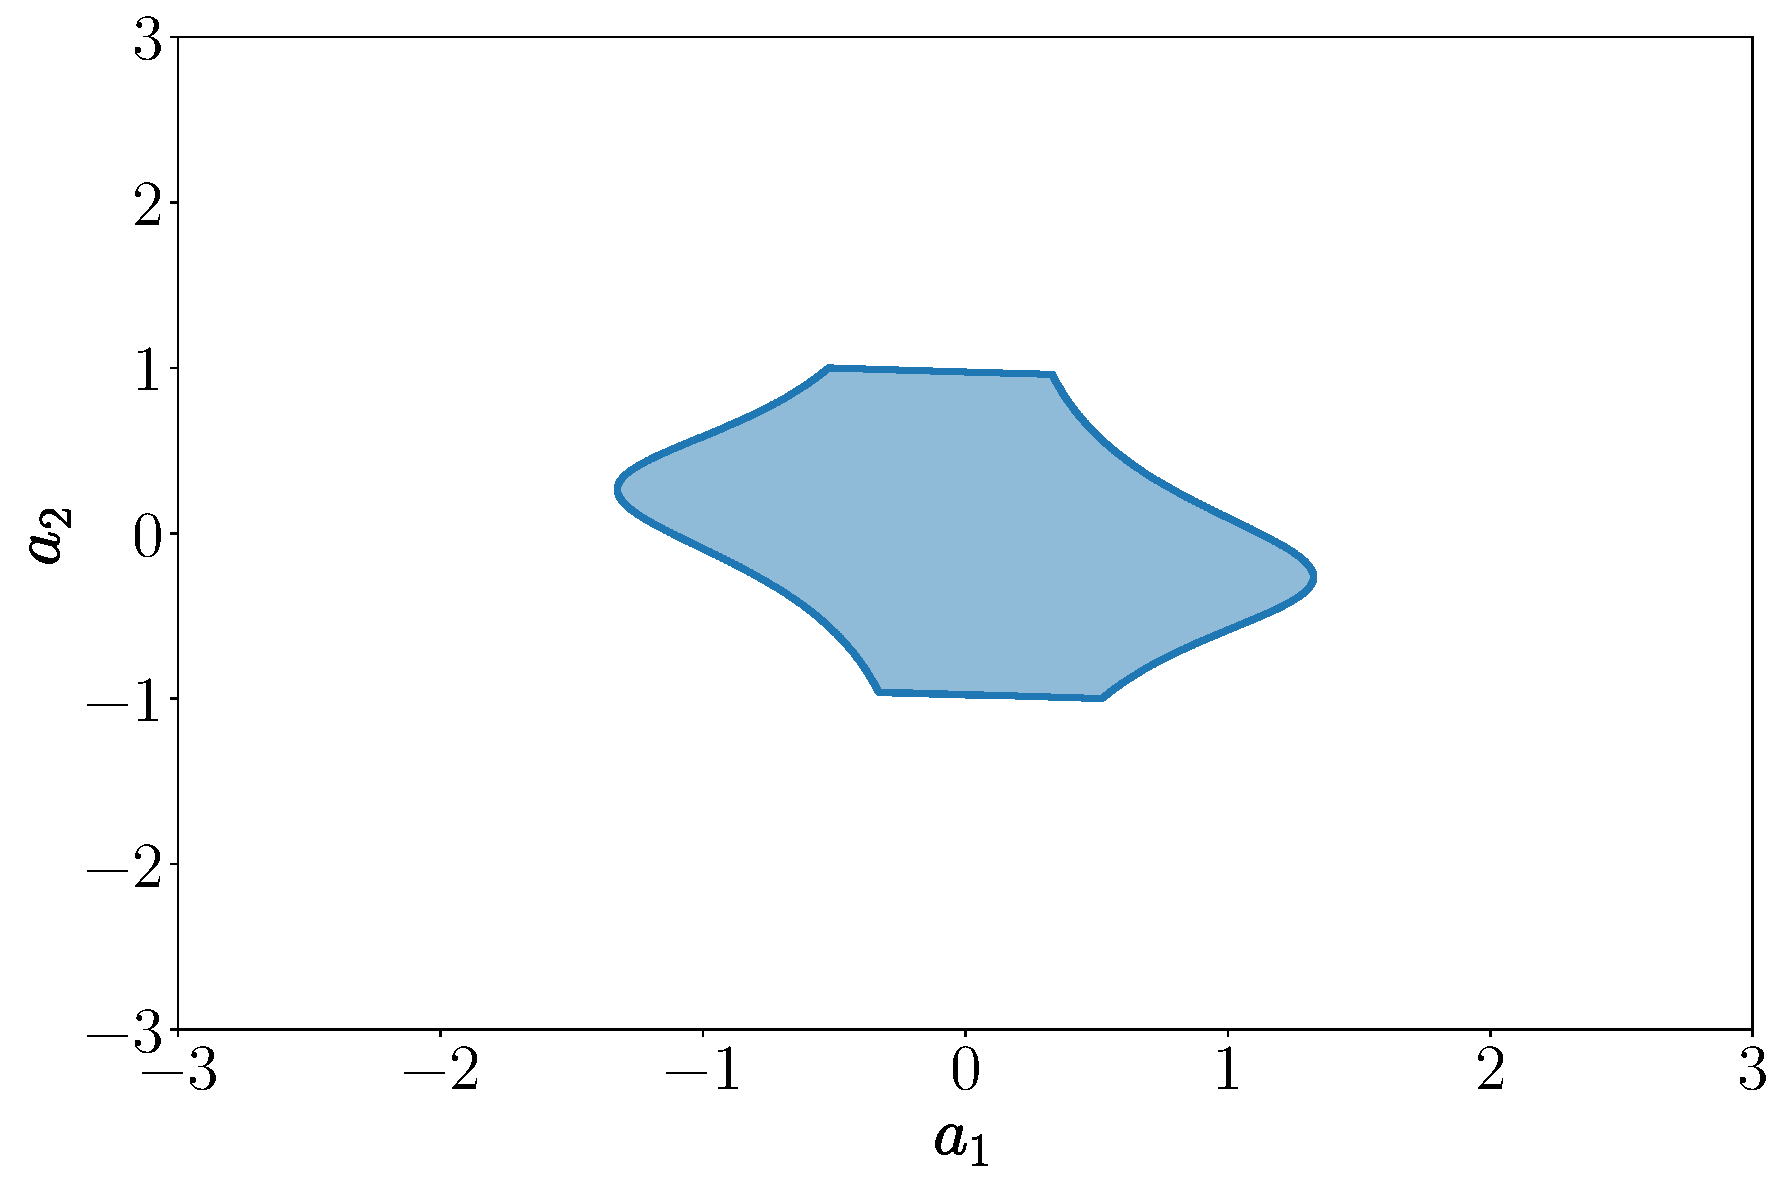
\includegraphics[scale = 0.15]{img/penrose_binaries/cmmr_joined_ergo/joined_ergo_b_0.93_q_0.1}
    \label{ch:penrose_binaries/fig:ergo_joined_d}
  }
  \subfloat[$b=0.93$, $q=0.5$]{
    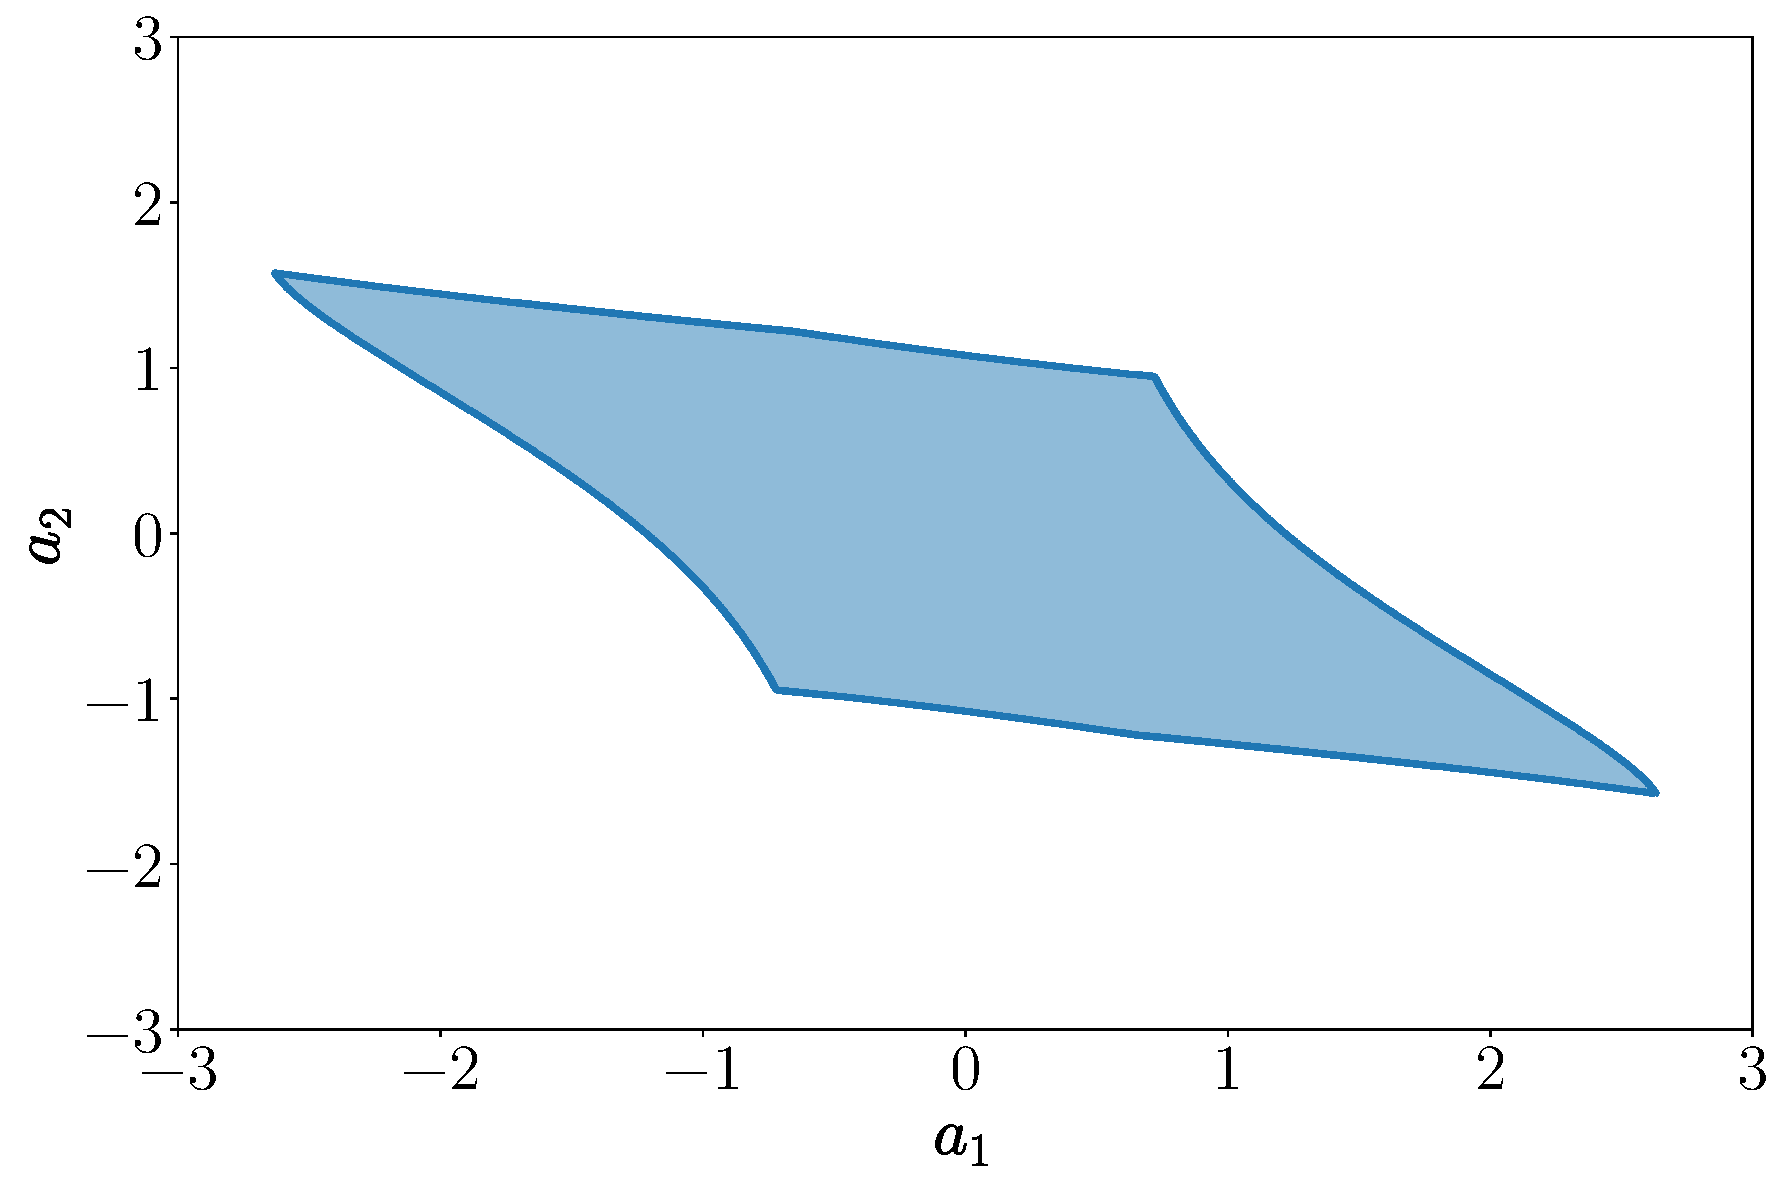
\includegraphics[scale = 0.15]{img/penrose_binaries/cmmr_joined_ergo/joined_ergo_b_0.93_q_0.5}
    \label{ch:penrose_binaries/fig:ergo_joined_e}
  }
  \subfloat[$b=0.93$, $q=1.0$]{
    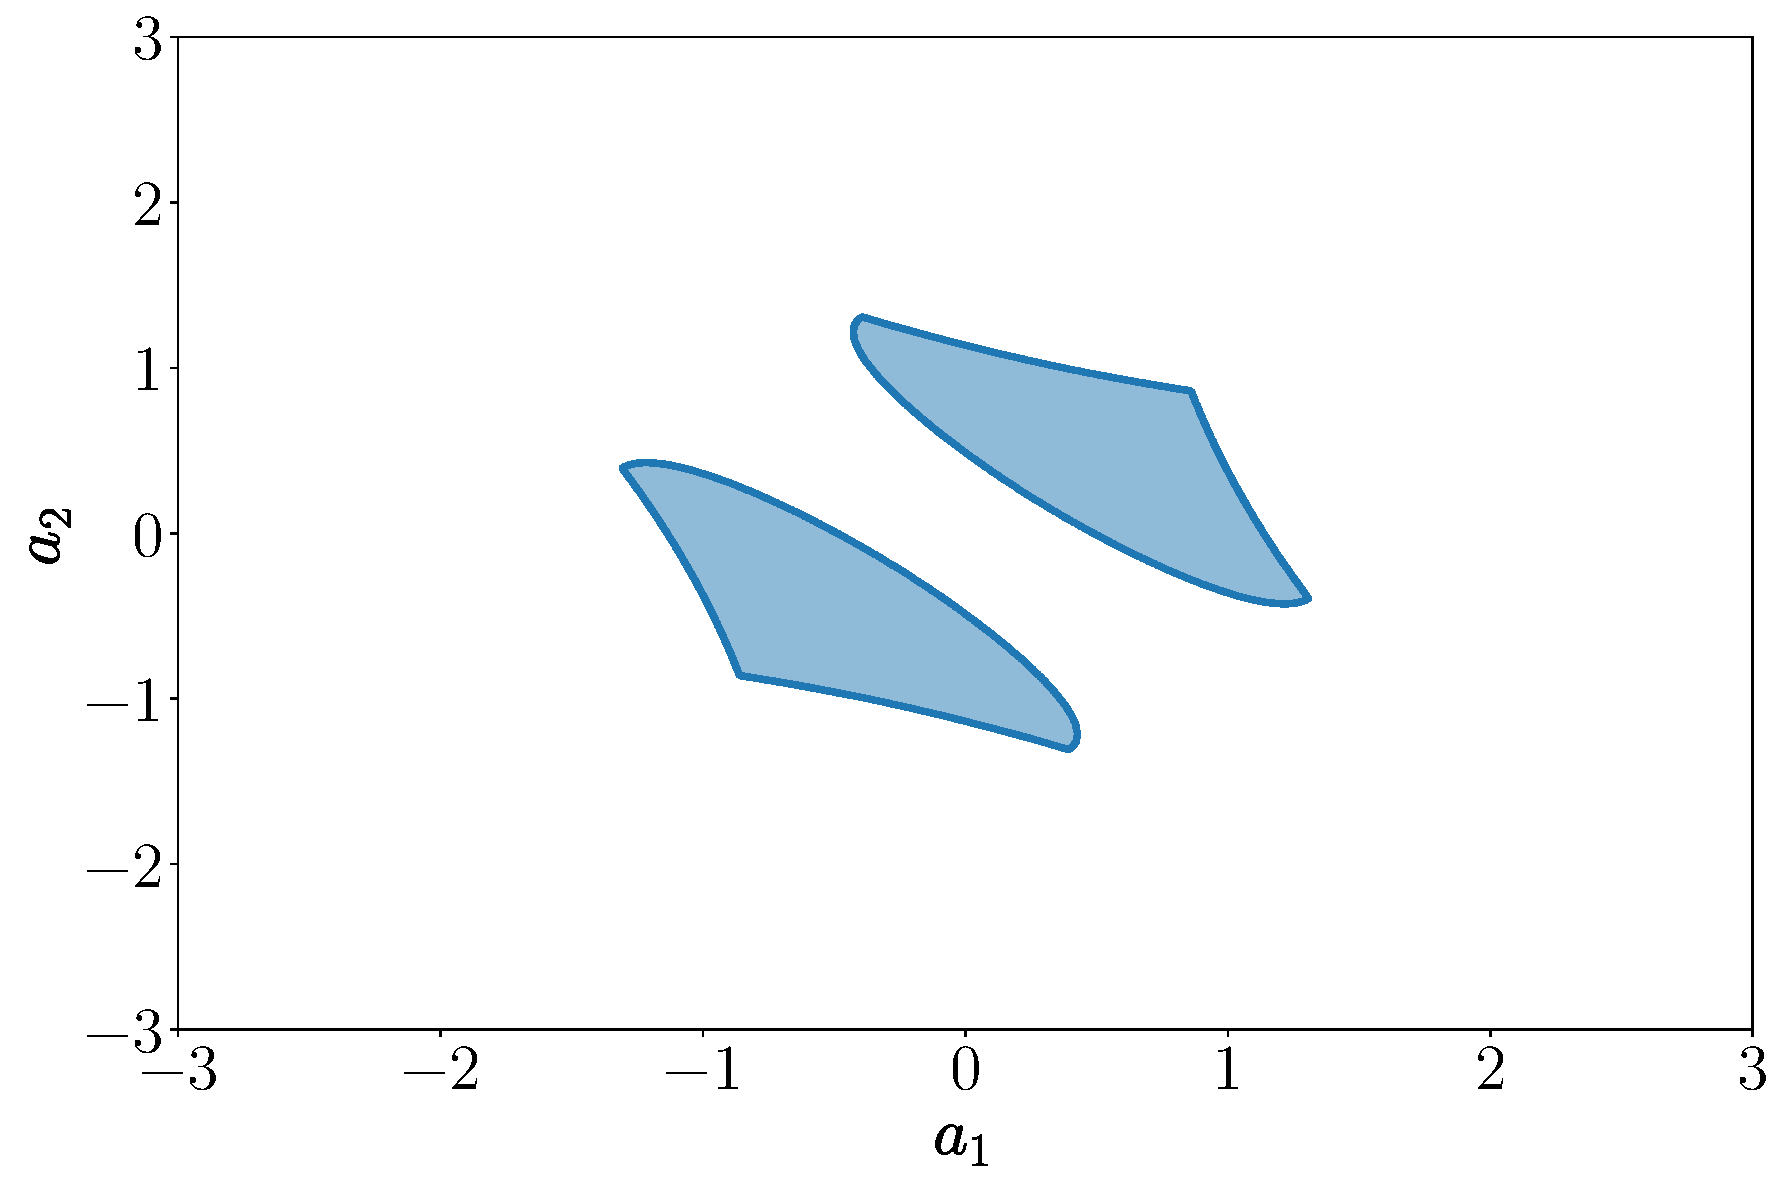
\includegraphics[scale = 0.15]{img/penrose_binaries/cmmr_joined_ergo/joined_ergo_b_0.93_q_1.0}
    \label{ch:penrose_binaries/fig:ergo_joined_f}
  }
  \newline
  \subfloat[$b=0.98$, $q=0.1$]{
    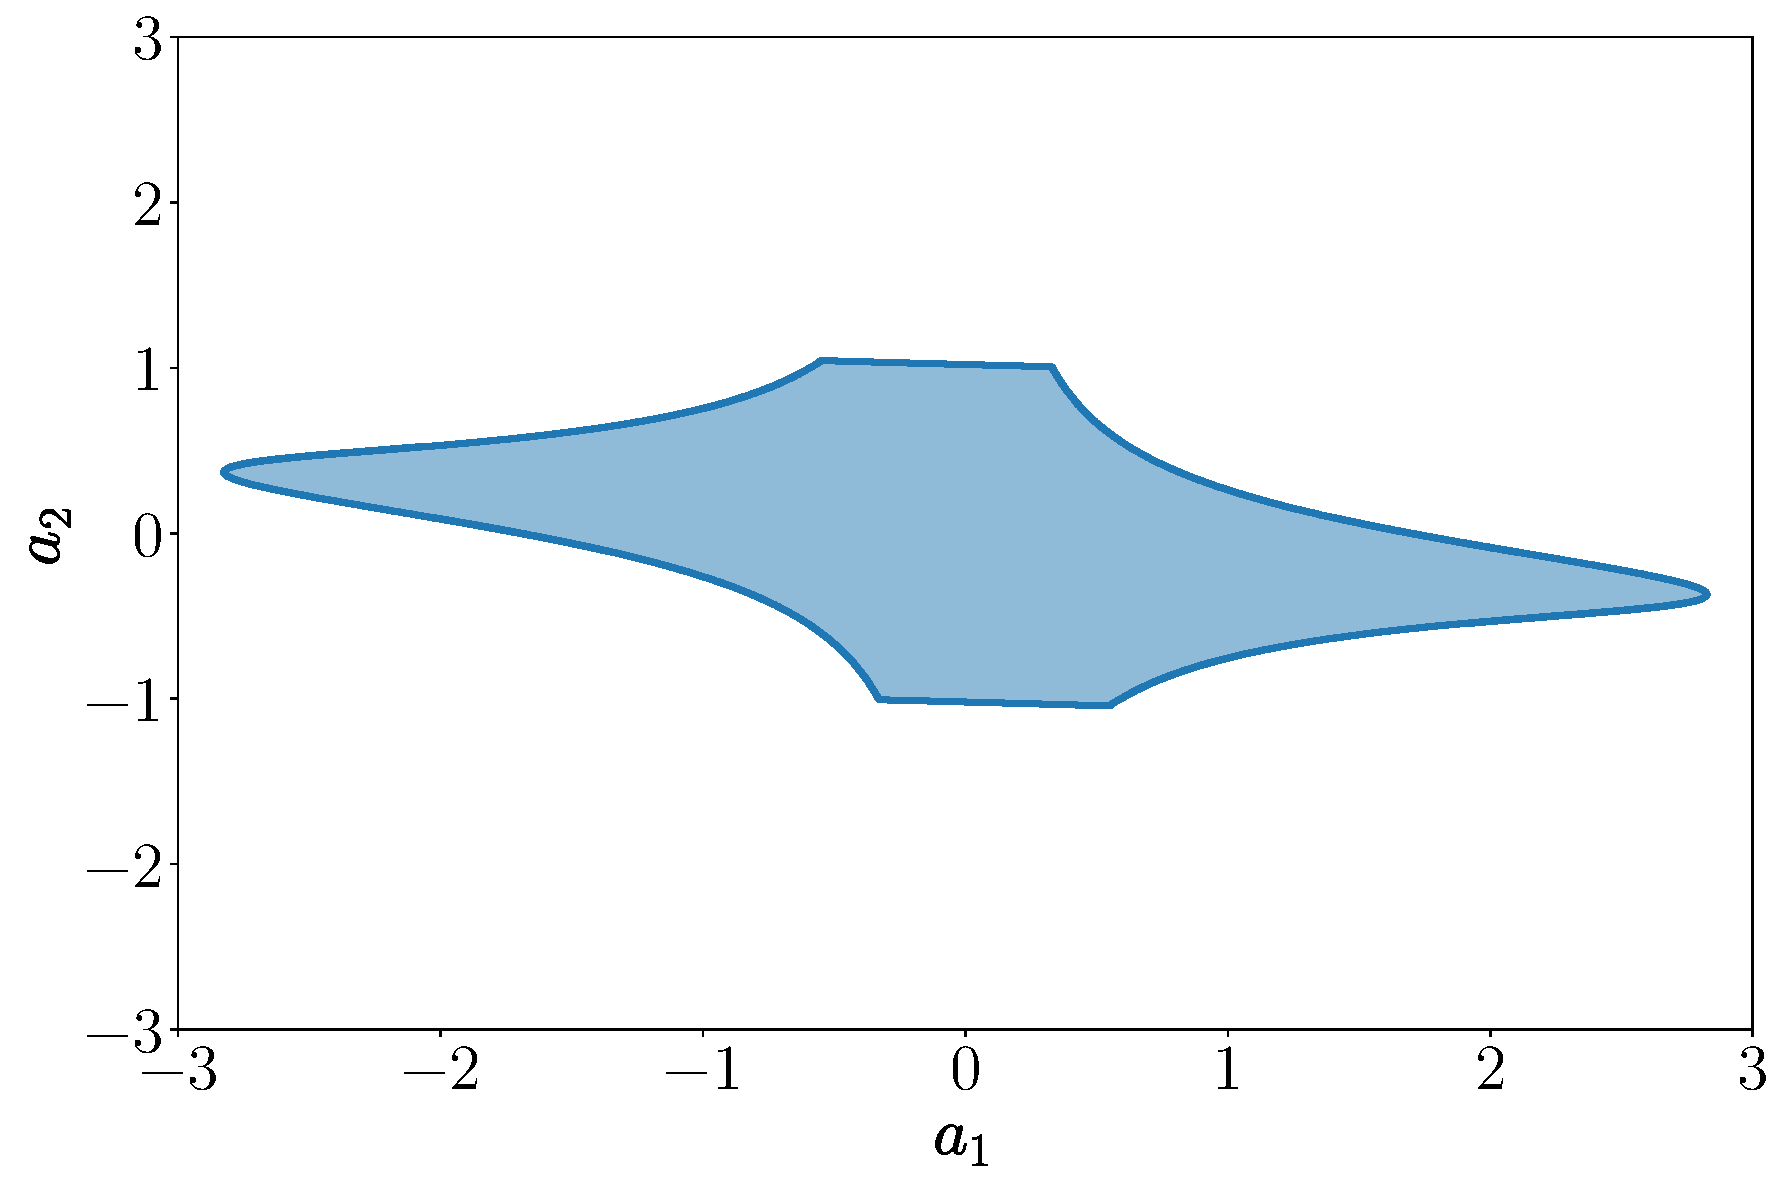
\includegraphics[scale = 0.15]{img/penrose_binaries/cmmr_joined_ergo/joined_ergo_b_0.98_q_0.1}
    \label{ch:penrose_binaries/fig:ergo_joined_g}
  }
  \subfloat[$b=0.98$, $q=0.5$]{
    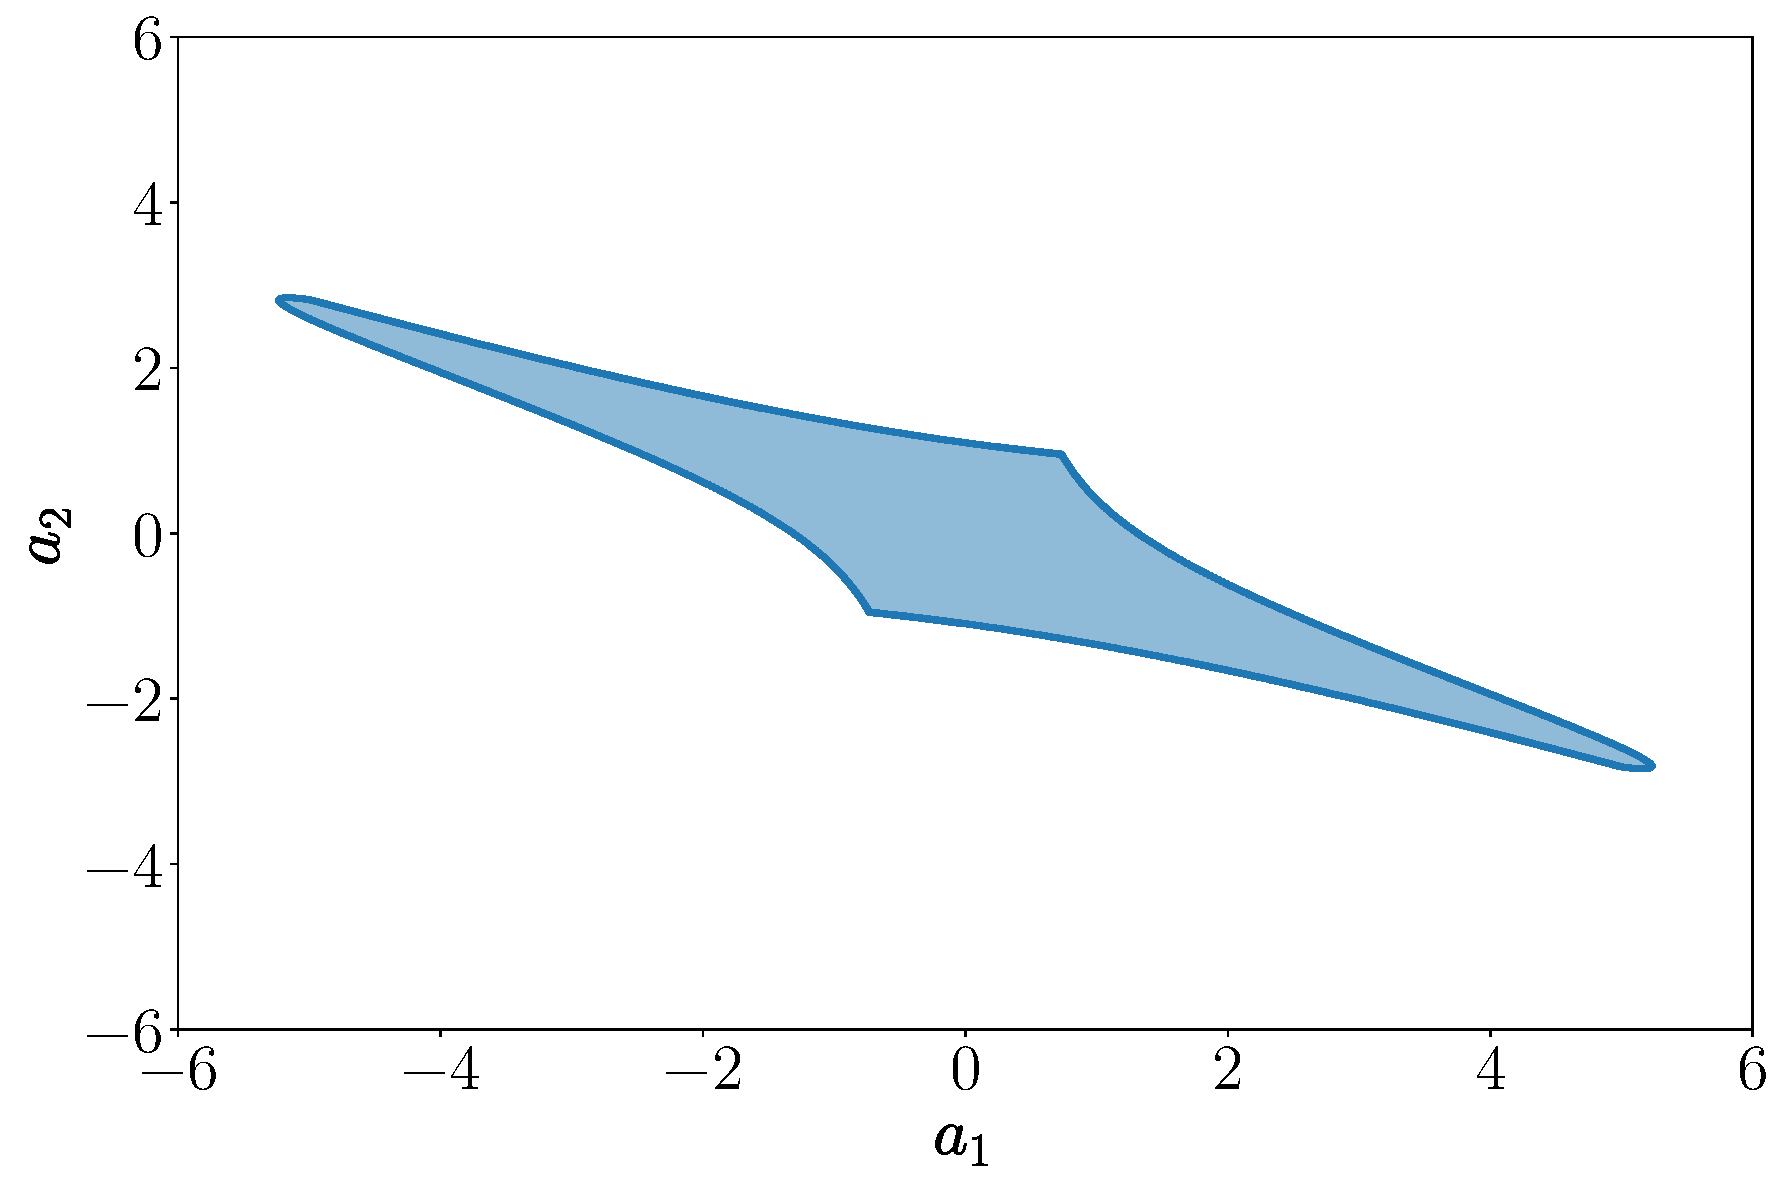
\includegraphics[scale = 0.15]{img/penrose_binaries/cmmr_joined_ergo/joined_ergo_b_0.98_q_0.5}
    \label{ch:penrose_binaries/fig:ergo_joined_h}
  }
  \subfloat[$b=0.98$, $q=1.0$]{
    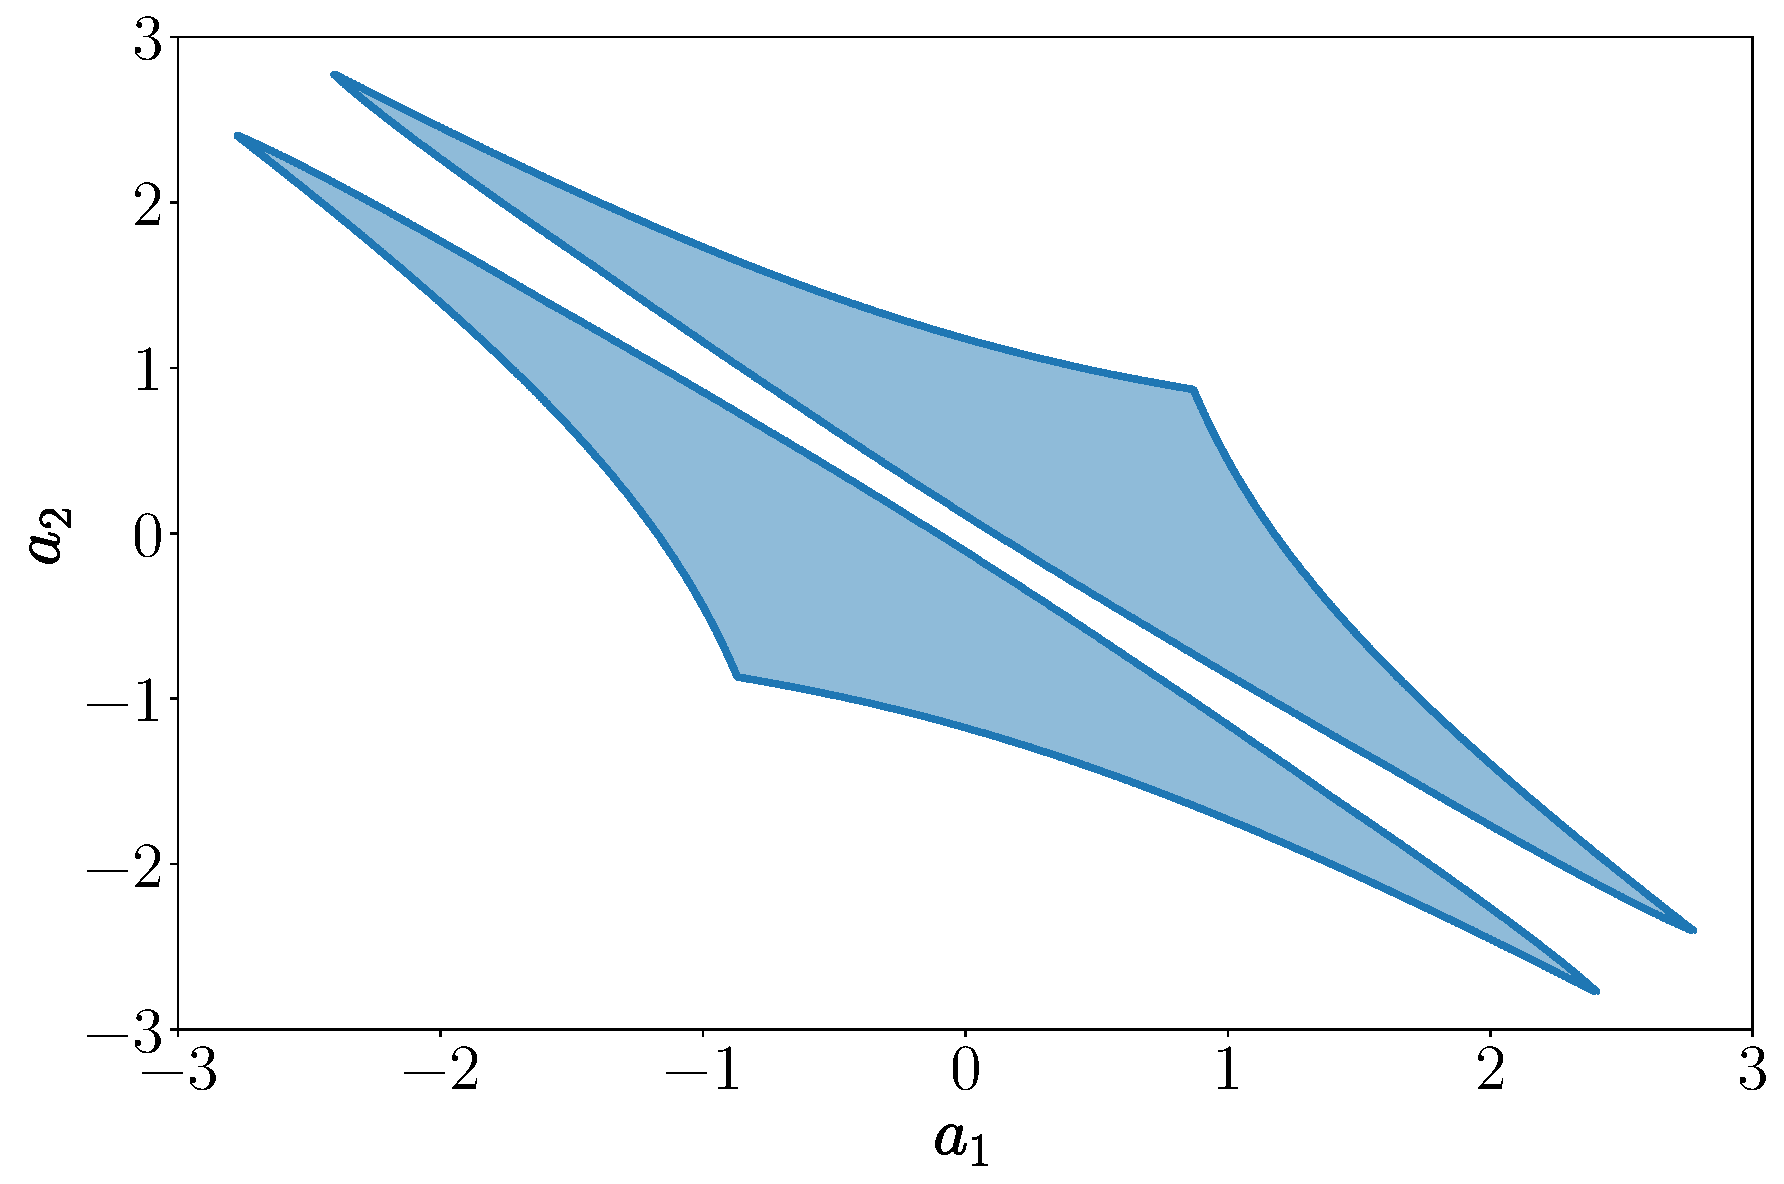
\includegraphics[scale = 0.15]{img/penrose_binaries/cmmr_joined_ergo/joined_ergo_b_0.98_q_1.0}
    \label{ch:penrose_binaries/fig:ergo_joined_i}
  }
  \caption{Parameter spaces that allow for a common ergosphere. The blue regions represent pairs of $a_1$ and $a_2$ values that produce an ergosphere around both black holes for each $(b,q)$  indicated value.}
  \label{ch:penrose_binaries/fig:ergo_joined}
\end{figure}

\begin{figure}
  \centering
  \subfloat[$a_1=1.0$, $q=0.5$]{
    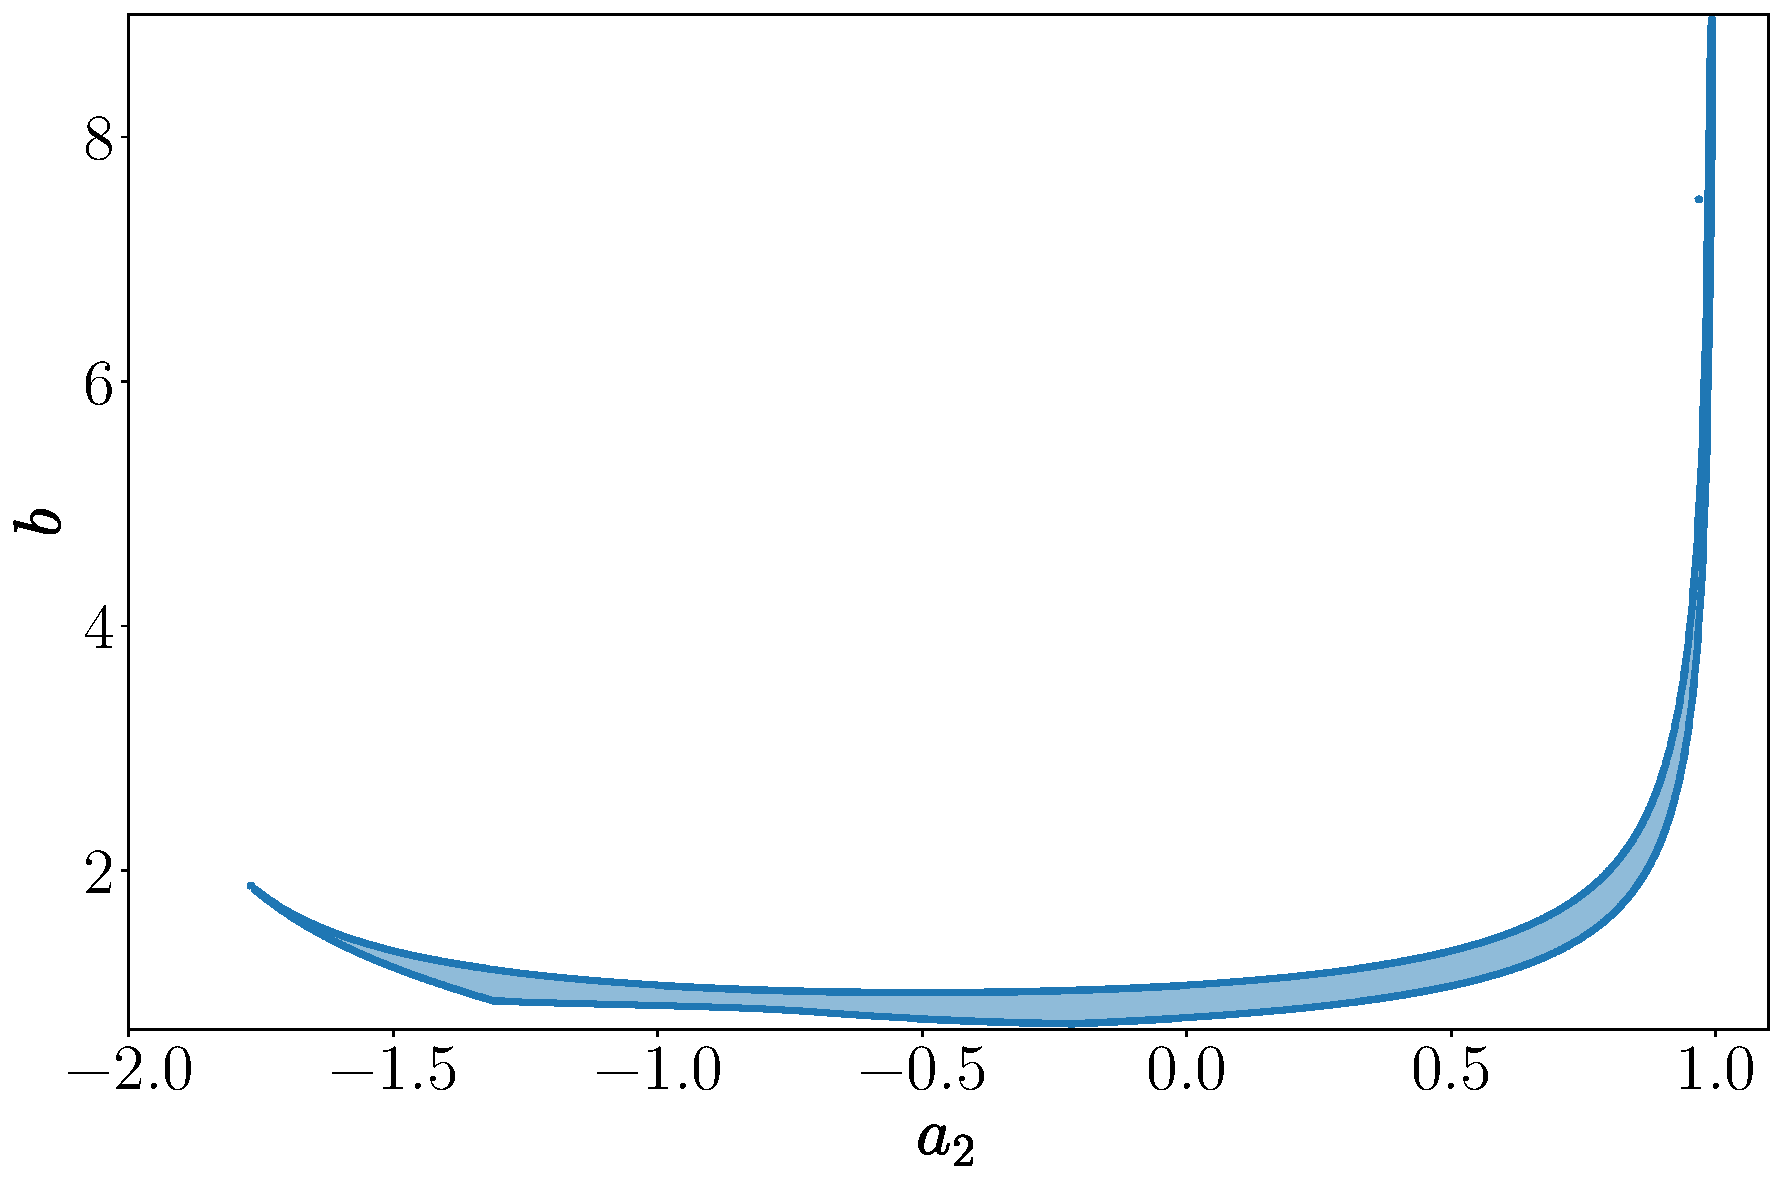
\includegraphics[scale = 0.22]{img/penrose_binaries/cmmr_joined_ergo/joined_ergo_2_a1_1.0_q_0.5.pdf}
    \label{ch:penrose_binaries/fig:ergo_joined_2_a}
  }
  \subfloat[$a_1=1.0$, $q=1.0$]{
    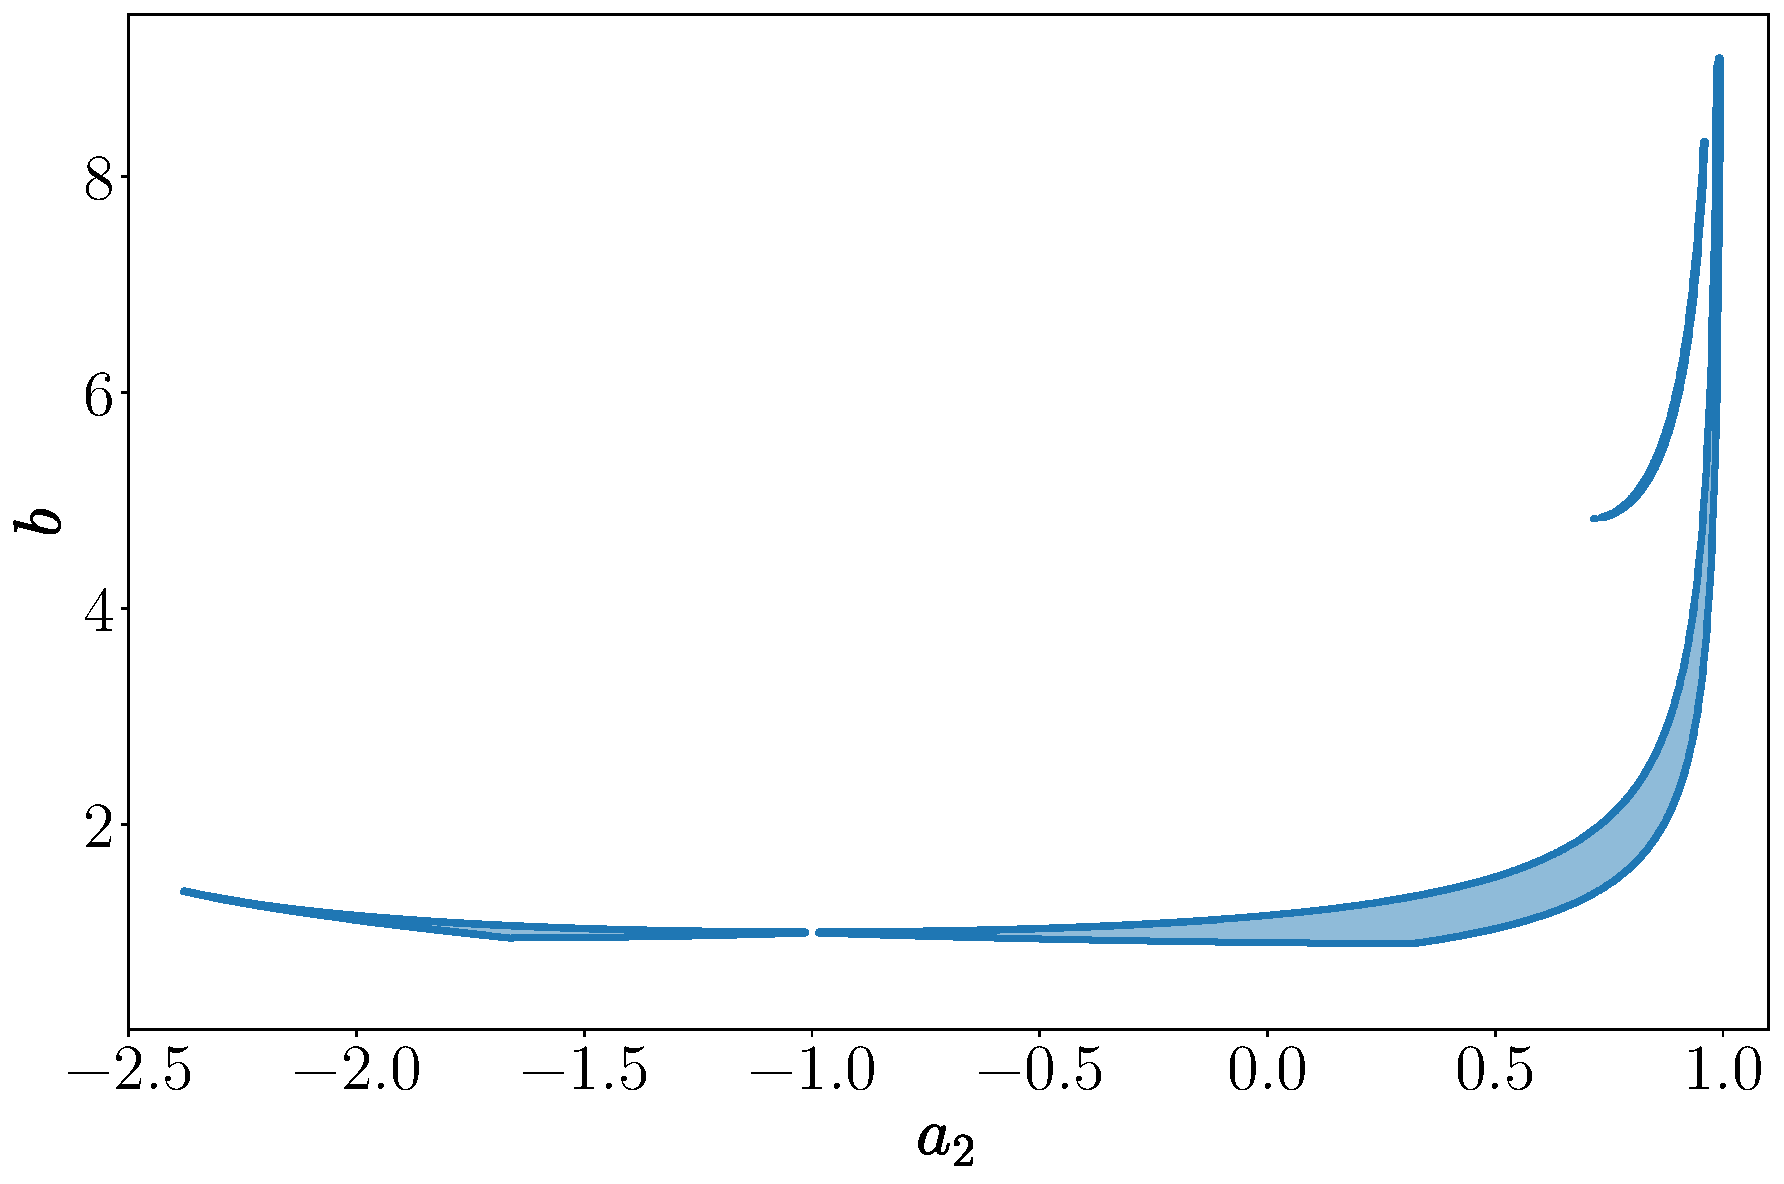
\includegraphics[scale = 0.22]{img/penrose_binaries/cmmr_joined_ergo/joined_ergo_2_a1_1.0_q_1.0.pdf}
    \label{ch:penrose_binaries/fig:ergo_joined_2_b}
  }
  \newline
  \subfloat[$a_1=1.5$, $q=0.5$]{
    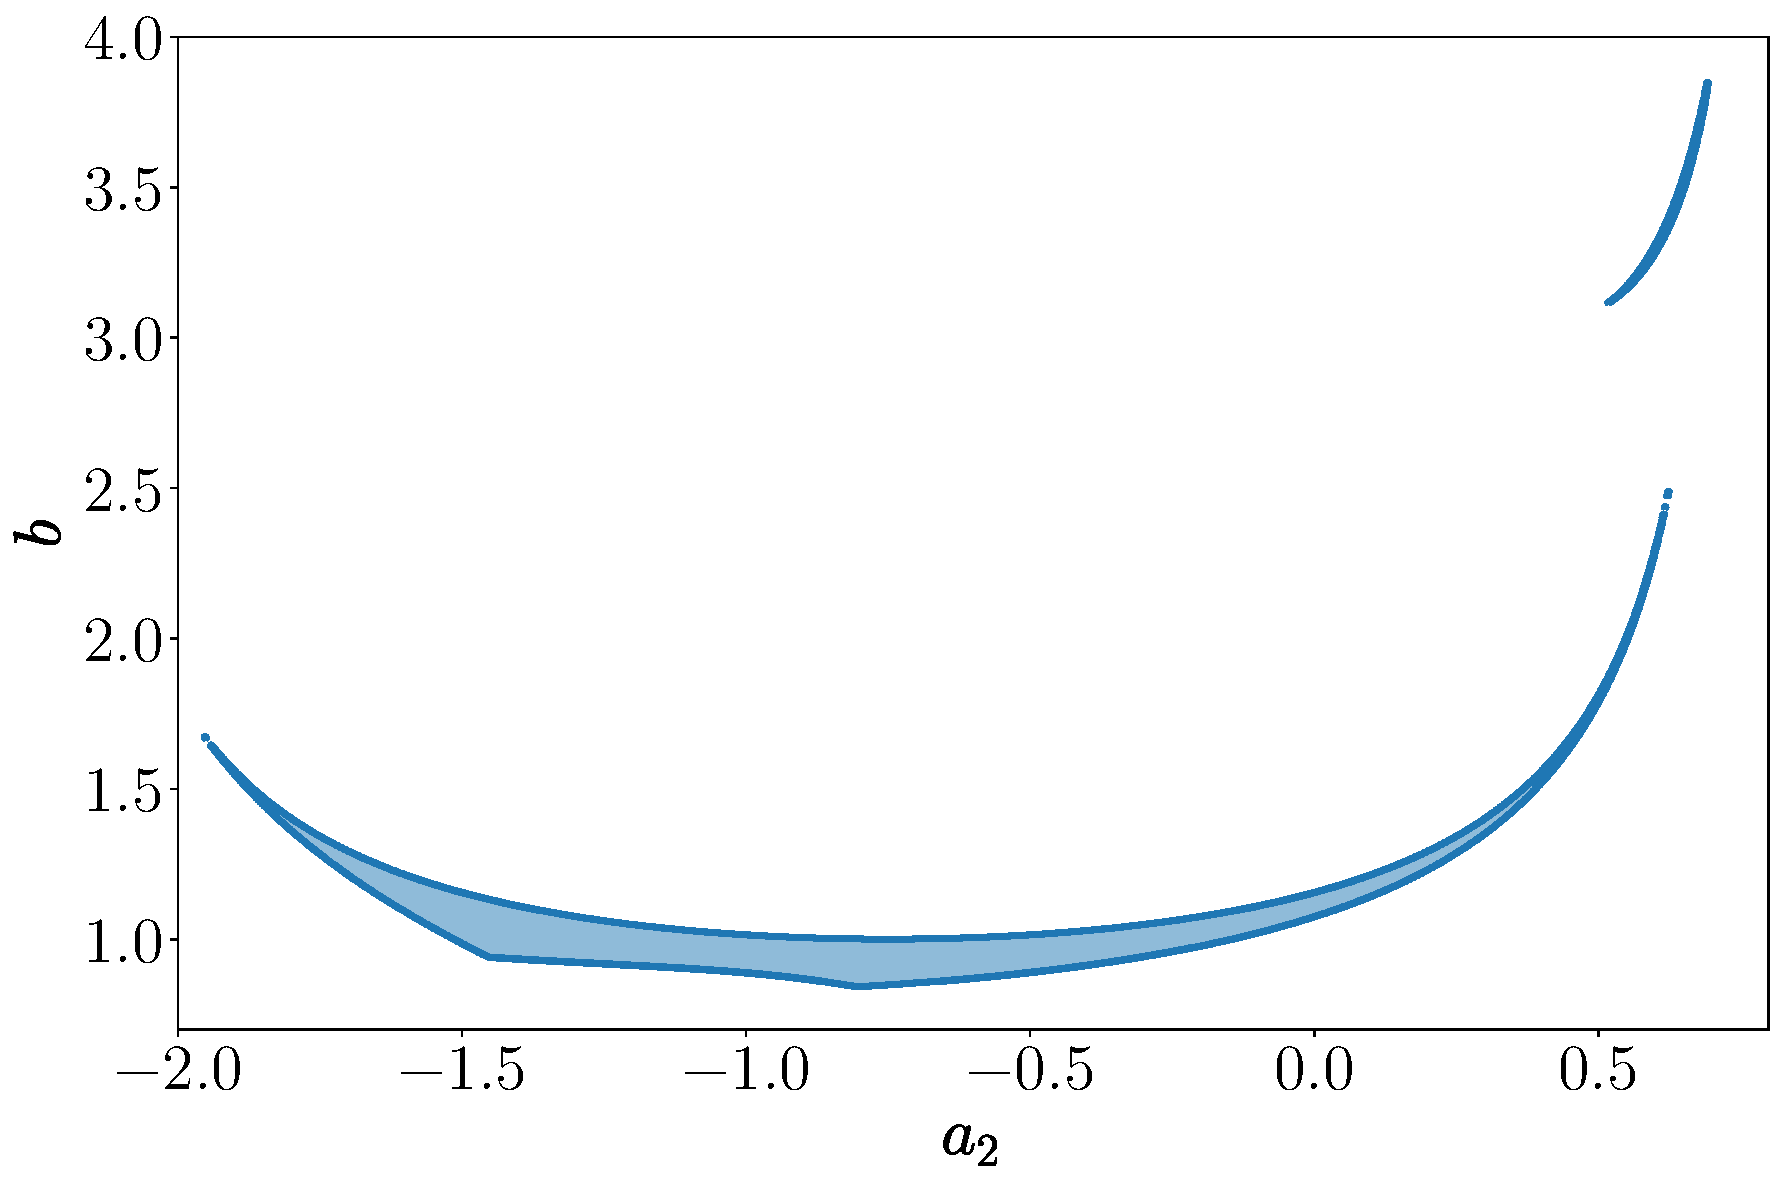
\includegraphics[scale = 0.22]{img/penrose_binaries/cmmr_joined_ergo/joined_ergo_2_a1_1.5_q_0.5.pdf}
    \label{ch:penrose_binaries/fig:ergo_joined_2_c}
  }
  \subfloat[$a_1=1.5$, $q=1.0$]{
    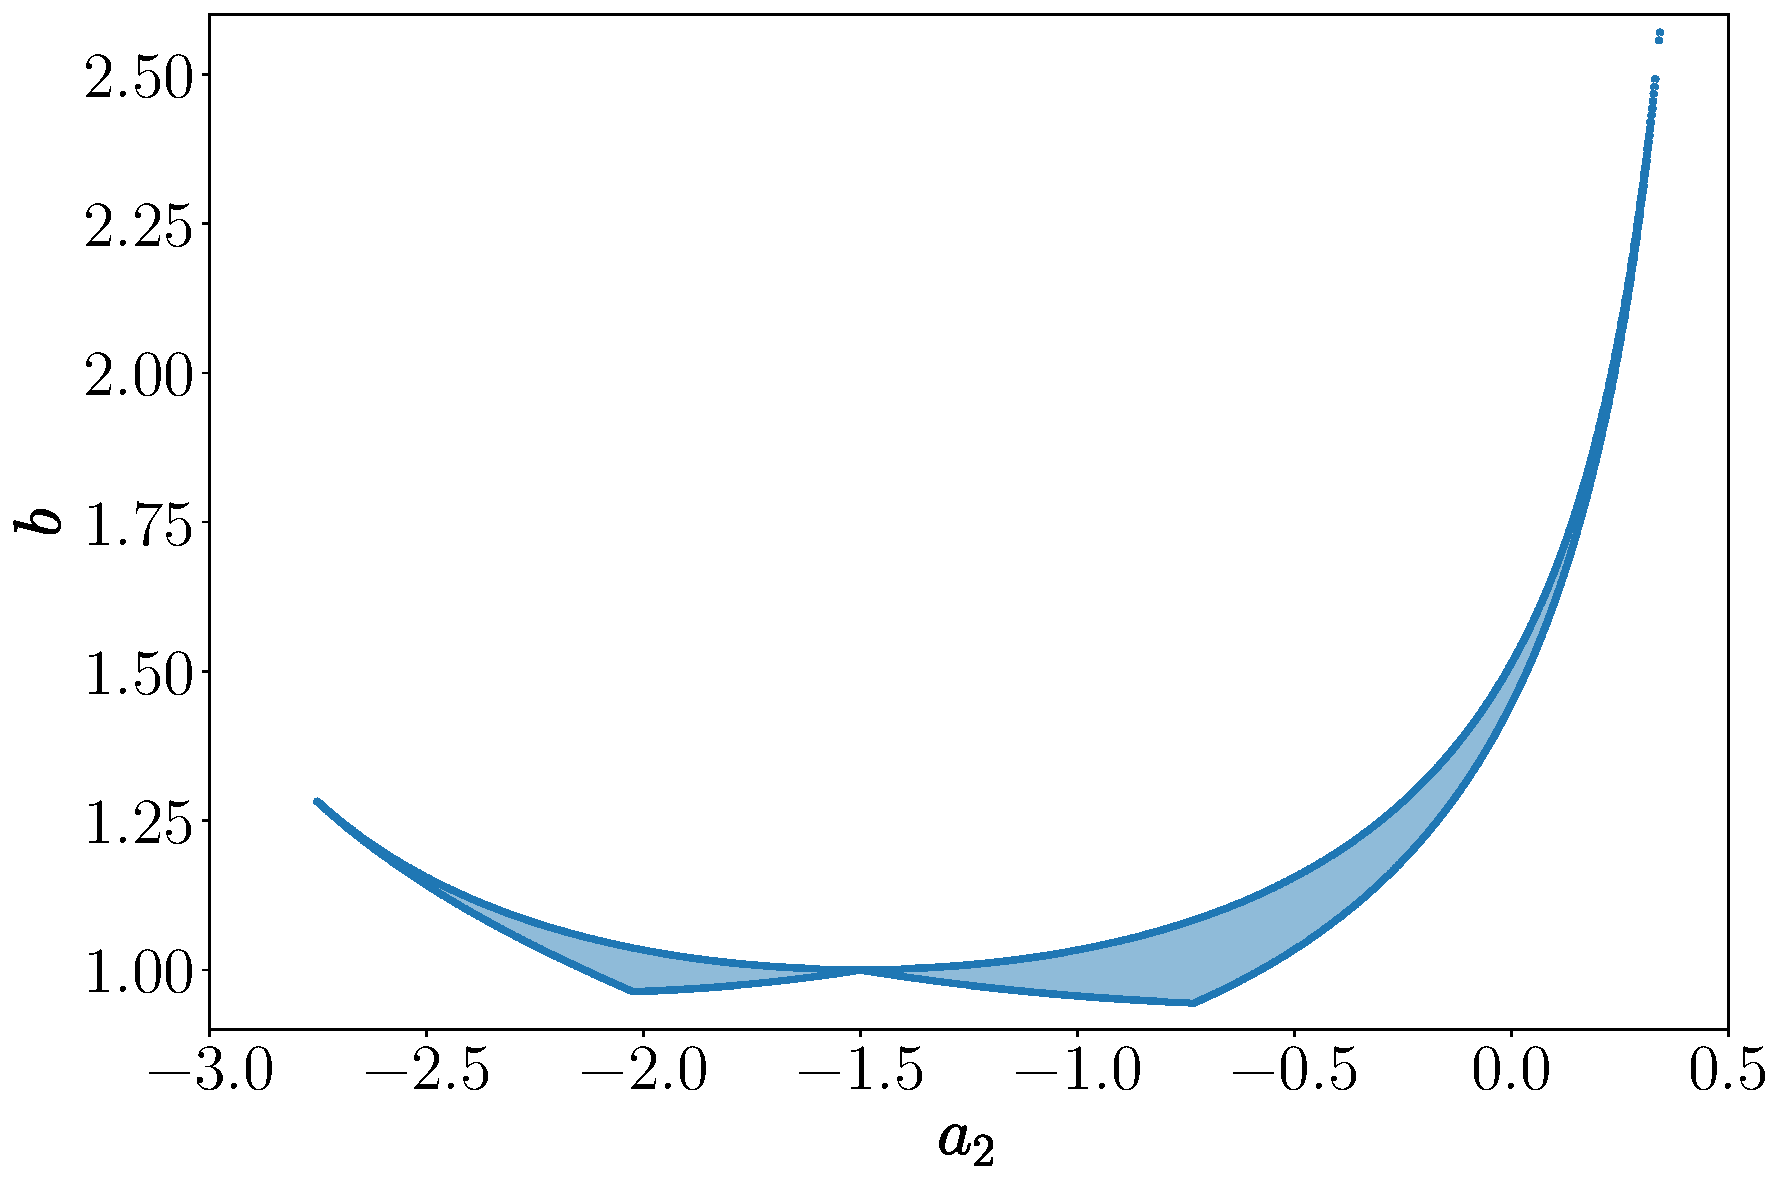
\includegraphics[scale = 0.22]{img/penrose_binaries/cmmr_joined_ergo/joined_ergo_2_a1_1.5_q_1.0.pdf}
    \label{ch:penrose_binaries/fig:ergo_joined_2_d}
  }
  \caption{Parameter spaces that allow for a common ergosphere. The blue regions represent pairs of $b$ and $a_2$ values that produce an ergosphere around both black holes for each $(a_1,q)$ indicated value.}
  \label{ch:penrose_binaries/fig:ergo_joined_2}
\end{figure}

\subsection{Geodesic motion in the $z=0$ plane}

We will make use of the Lagrangian formalism to determine the form of the geodesic equations and the motion's conserved quantities. Letting a dot represent derivatives with respect to the proper time we can write the Lagrangian of the geodesic motion as~\cite{carroll}
%
\begin{equation}
  2\mathcal{L} = -f(\dot{t} - \omega\dot{\varphi})^2 +f^{-1}\left[e^{2\gamma}\left( \dot{\rho}^2 + \dot{z}^2 \right) + \rho^2\dot{\varphi}^2 \right].
  \label{ch:penrose_binaries/eq:lagrangian}
\end{equation}

From \myref{ch:penrose_binaries/eq:lagrangian} we can identify two constants of the motion, the energy per unit mass as measured by a static observer at infinity $E$, given by
%
\begin{equation}
  E = f\dot{t} - \omega f\dot{\varphi}
  \label{ch:penrose_binaries/eq:energy_t_phi}
\end{equation}
%
and the angular momentum about the $z$ axis per unit mass as measured by a static observer at infinity $L$, given by
%
\begin{equation}
  L = \omega f \dot{t} + \left( \frac{\rho^2}{f} - \omega^2 f \right)\dot{\varphi}.
  \label{ch:penrose_binaries/eq:ang_mom_t_phi}
\end{equation}

We can use Eqs.~\eqref{ch:penrose_binaries/eq:energy_t_phi} and \eqref{ch:penrose_binaries/eq:ang_mom_t_phi} to find $\dot{t}$ and $\dot{\varphi}$, in terms of $E$ and $L$ which yield
%
\begin{equation}
  \dot{t} = \frac{E}{f} + \frac{\omega f (L - E\omega)}{\rho^2}
  \label{ch:penrose_binaries/eq:t_dot}
\end{equation}
%
and
%
\begin{equation}
  \dot{\varphi} = \frac{f (L - E\omega)}{\rho^2}
  \label{ch:penrose_binaries/eq:phi_dot}
\end{equation}

A third conserved quantity is the normalization of the four velocity for a massive particle, that is, $\mtrtens{\mu}{\nu}\dot{x}^\mu\dot{x}^\nu = -1$ which can be combined with Eqs.~\eqref{ch:penrose_binaries/eq:t_dot} and \eqref{ch:penrose_binaries/eq:phi_dot} to produce an expression for the particle's energy in terms of its ``spatial'' four velocities ($\dot{\rho}$ and $\dot{z}$) and it's angular momentum $L$, yielding
%
\begin{multline}
  E = \frac{-f^2\omega L}{\rho^2-\omega^2 f^2} + \left[ \frac{\rho^2e^{2\gamma}(\dot{\rho}^2 + \dot{z}^2)}{\rho^2 - \omega^2f^2} + \left( \frac{\rho fL}{\rho^2 - \omega^2f^2} \right)^2 \right. \\
  \left. + \frac{\rho^2f}{\rho^2 - \omega^2f^2} \right]^{1/2}
  \label{ch:penrose_binaries/eq:energy_rho_z}
\end{multline}
%
where the positive sign is chosen for the square root to guarantee that a static particle at infinity has positive energy.

By inverting Eq.~\eqref{ch:penrose_binaries/eq:energy_rho_z} to obtain $\dot{\rho}^2 + \dot{z}^2$ we are motivated to define the effective potential
%
\begin{equation}
  V_{\text{eff}} = \frac{\rho^2 - \omega^2 f^2}{\rho^2 e^{2\gamma}}\left[ \left( \frac{\rho fL}{\rho^2 - \omega^2f^2} \right)^2 + \frac{\rho^2f}{\rho^2 - \omega^2f^2}\right]
  \label{ch:penrose_binaries/eq:effective_potential}
\end{equation}
%
and the effective energy
%
\begin{equation}
  E_{\text{eff}} = \frac{\rho^2 - \omega^2 f^2}{\rho^2 e^{2\gamma}}\left(E + \frac{f^2\omega L}{\rho^2-\omega^2 f^2}\right)^2
  \label{ch:penrose_binaries/eq:effective_energy}
\end{equation}
%
and therefore we can write
%
\begin{equation}
  \dot{\rho}^2 + \dot{z}^2 = E_{\text{eff}} - V_{\text{eff}}.
  \label{ch:penrose_binaries/eq:effective_potential_motion}
\end{equation}

Finally, the geodesic equations can be derived using the Euler-Lagrange equations for the Lagrangian of Eq.~\eqref{ch:penrose_binaries/eq:lagrangian} and $\dot{t}$ and $\dot{\varphi}$ can be replaced with Eqs.~\eqref{ch:penrose_binaries/eq:t_dot} and \eqref{ch:penrose_binaries/eq:phi_dot}, respectively. While studying geodesic motion in binary system of two identical Kerr-Newman black holes held by a massless strut (a solution with the same general line element as Eq.~\eqref{ch:penrose_binaries/eq:line_element}) the authors of Ref.~\cite{Dubeibe2016} in Eqs.~(16) and (17) derive the explicit form of the geodesic equations for $\rho$ and $z$ in terms of $E$, $L$ and the metric functions $f$, $\omega$ and $e^{2\gamma}$ and thus we shall not repeat this information here. In our work, whenever was necessary to solve the geodesic equations numerically we implemented Eqs.~(16) and (17) of Ref.~\cite{Dubeibe2016} directly, changing only the metric functions to those described in  Sec.~IV of Ref.~\cite{MANKO2020}.

If the motion is constrained to the $z=0$ symmetry plane, we can easily determine the general characteristics of massive particle geodesics by plotting the effective potential, Eq.~\eqref{ch:penrose_binaries/eq:effective_potential}, as was done in Fig.~\ref{ch:penrose_binaries/fig:effective_potential}. The different curves represent different values of angular momenta, specifically $L = 18$ in the black curve, $L = 13$ in the red curve, $L=10$ in the blue curve and $L=4$ in the green curve. We can see that both stable and unstable circular orbits are possible, as well as escaping orbits and non-circular bounded orbits that become ``wider'' as the value of $L$ decreases.

\begin{figure}
  \centering
  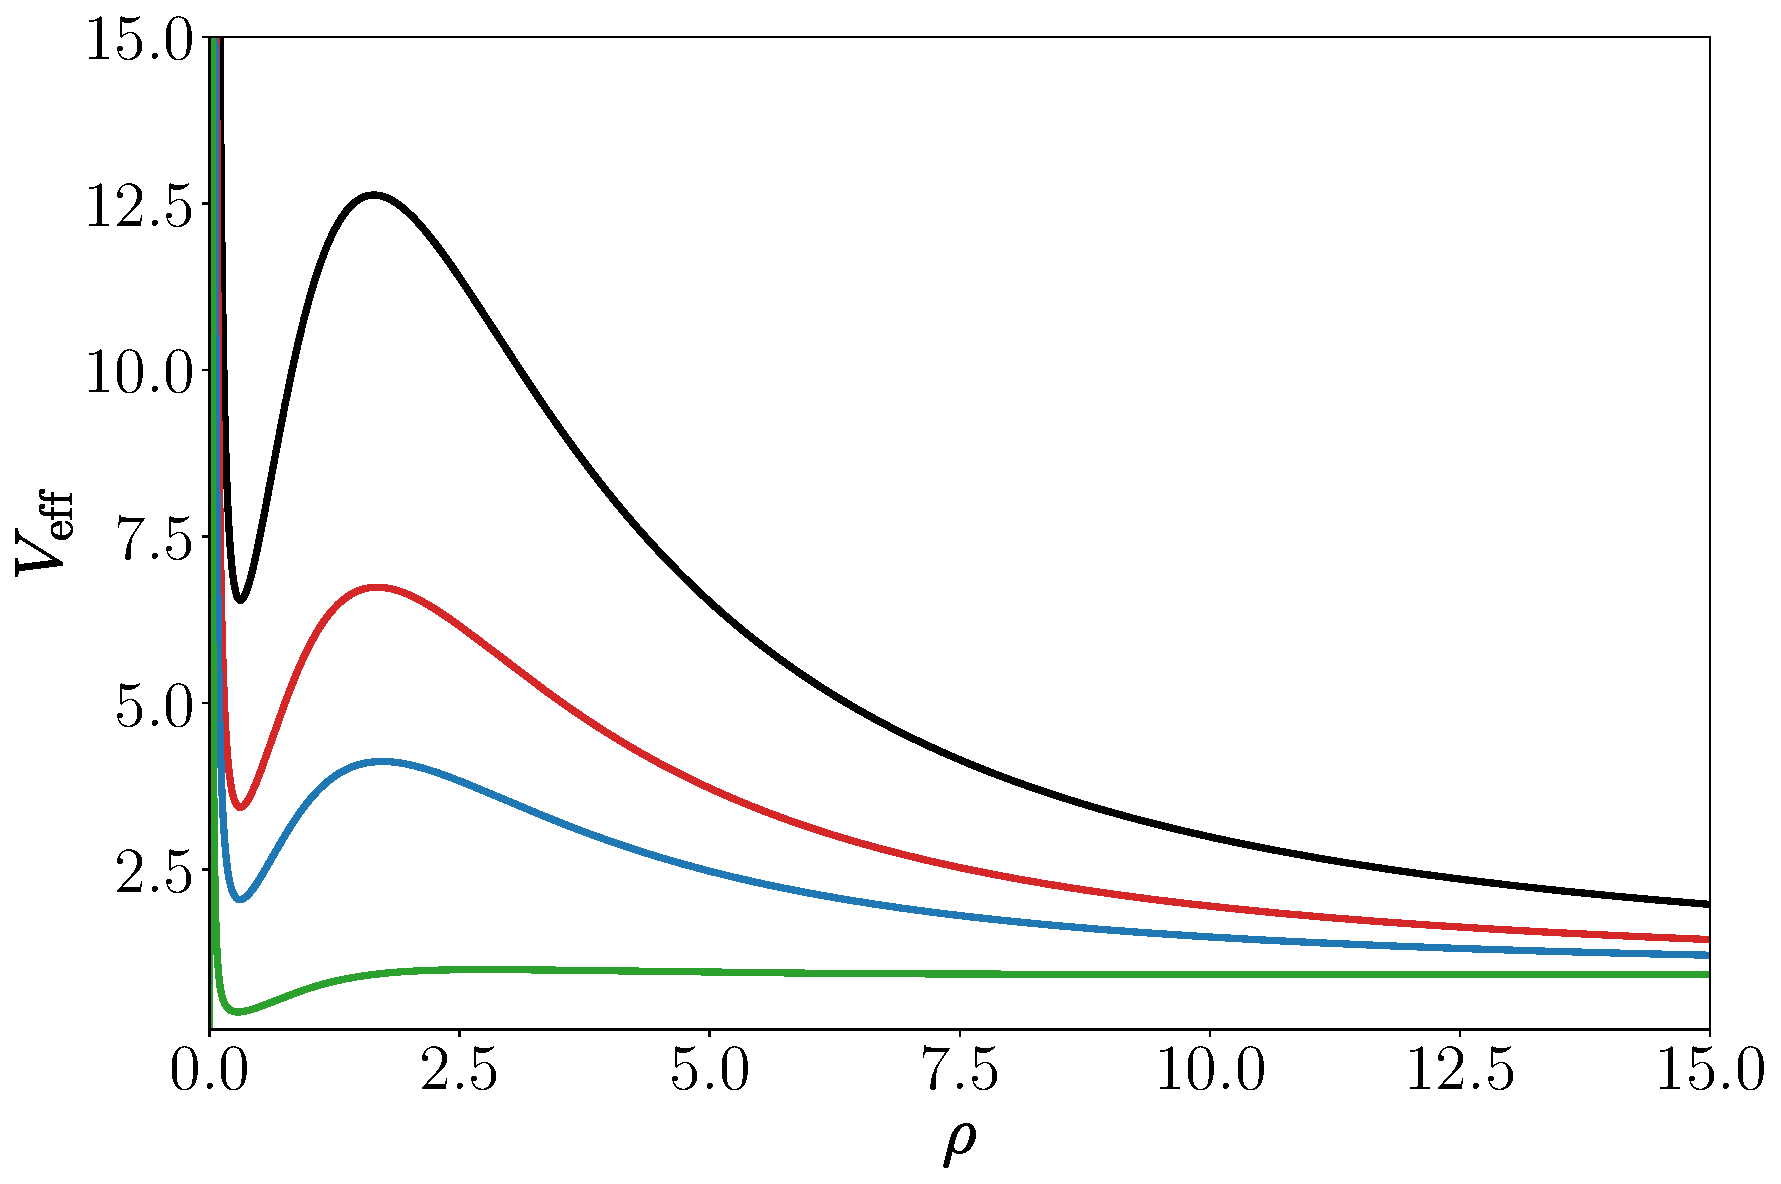
\includegraphics[scale = 0.3]{img/penrose_binaries/cmmr_vEff.pdf}
  \caption{Effective potential in the $z=0$ plane for $L=18,13,10$ and $4$ (black, red, blue and green curves respectively).}
  \label{ch:penrose_binaries/fig:effective_potential}
\end{figure}

\subsection{Negative energy orbits}

Now we turn our attention to the conditions required for a orbit to have negative energy for a static observer at infinity, as this is a necessary condition for the occurrence of the Penrose process. By inspecting Eq.~\eqref{ch:penrose_binaries/eq:energy_rho_z} we can immediately conclude that since the term in the square root is always positive, a necessary (but not sufficient) condition for the particle's energy to be negative is that
%
\begin{equation}
  \frac{-f^2\omega L}{\rho^2 - \omega^2 f^2} < 0.
  \label{ch:penrose_binaries/eq:necessary_condition}
\end{equation}
%
Multiplying both sides by the denominator we conclude that the numerator must be negative. Because $-f^2$ is always negative, the necessary condition for the existence of negative energy orbits is that
%
\begin{equation}
  (\omega < 0 \land L > 0) \lor (\omega > 0 \land L < 0)
\end{equation}
%
which simply means that the horizons must rotate in the opposite direction of the particles own rotation.

Despite $\omega(\rho,z)$ being know analytically, it's complexity does not allow us to easily reason about it's behaviour and thus we proceeded to visualize it numerically employing the same projection scheme in the Cartesian plane as was done in the visualisation of the ergosphere. With that we obtain Fig.~\ref{ch:penrose_binaries/fig:omega_value_regions}. The color indicates the value of $\omega$ at each point $(x,y)$ and the values that were graphed were deliberately chosen to lie in the range $-25 \leq \omega \leq 25$ in order to facilitate the visualization. In all panels we choose $b=0.98$ and $q=1.0$. The upper left panel shows a configuration with aligned spins $a_1=a_2=0.65$ and the upper right shows the equivalent configuration with anti-aligned spins $-a_1=a_2=0.65$. The lower row shows binaries with anti-aligned but very different spins with $a_1=0.65$ and $a_2=-0.1$ in the left panel and $a_1=-0.65$ and $a_2 = 0.1$ in the right panel. In all cases the green curve marks the boundary of the ergosphere and the black lines mark the event horizons.

From Fig.~\ref{ch:penrose_binaries/fig:omega_value_regions} it becomes clear that in the case of a system with aligned or anti aligned but very different spins one can extract energy from either of the two black holes by setting the sign of $L$ to be opposite to that of $\omega$ inside the ergosphere. The black hole that will ultimately loose part of it's energy can then only be determined uniquely from the other dynamical parameters of the particle's trajectory. In the case of anti-aligned but equal or similar spins the sign of $L$ determines uniquely which black hole can be used for energy extraction, which will be either the upper or lower black hole, depending on the sign configurations of $\omega$ and $L$ inside the ergosphere. This feature is completely compatible with the notion that energy can only be extracted inside the ergospehre. For spin configurations in which a single ergosphere exists around both black holes, energy can be extracted from either hole while in configurations in which the ergospheres are located around each hole but are disconnected, energy can be extracted from only one of the constituents.

\begin{figure}
  \centering
  \subfloat[$a_1 = a_2 = 0.65$]{
    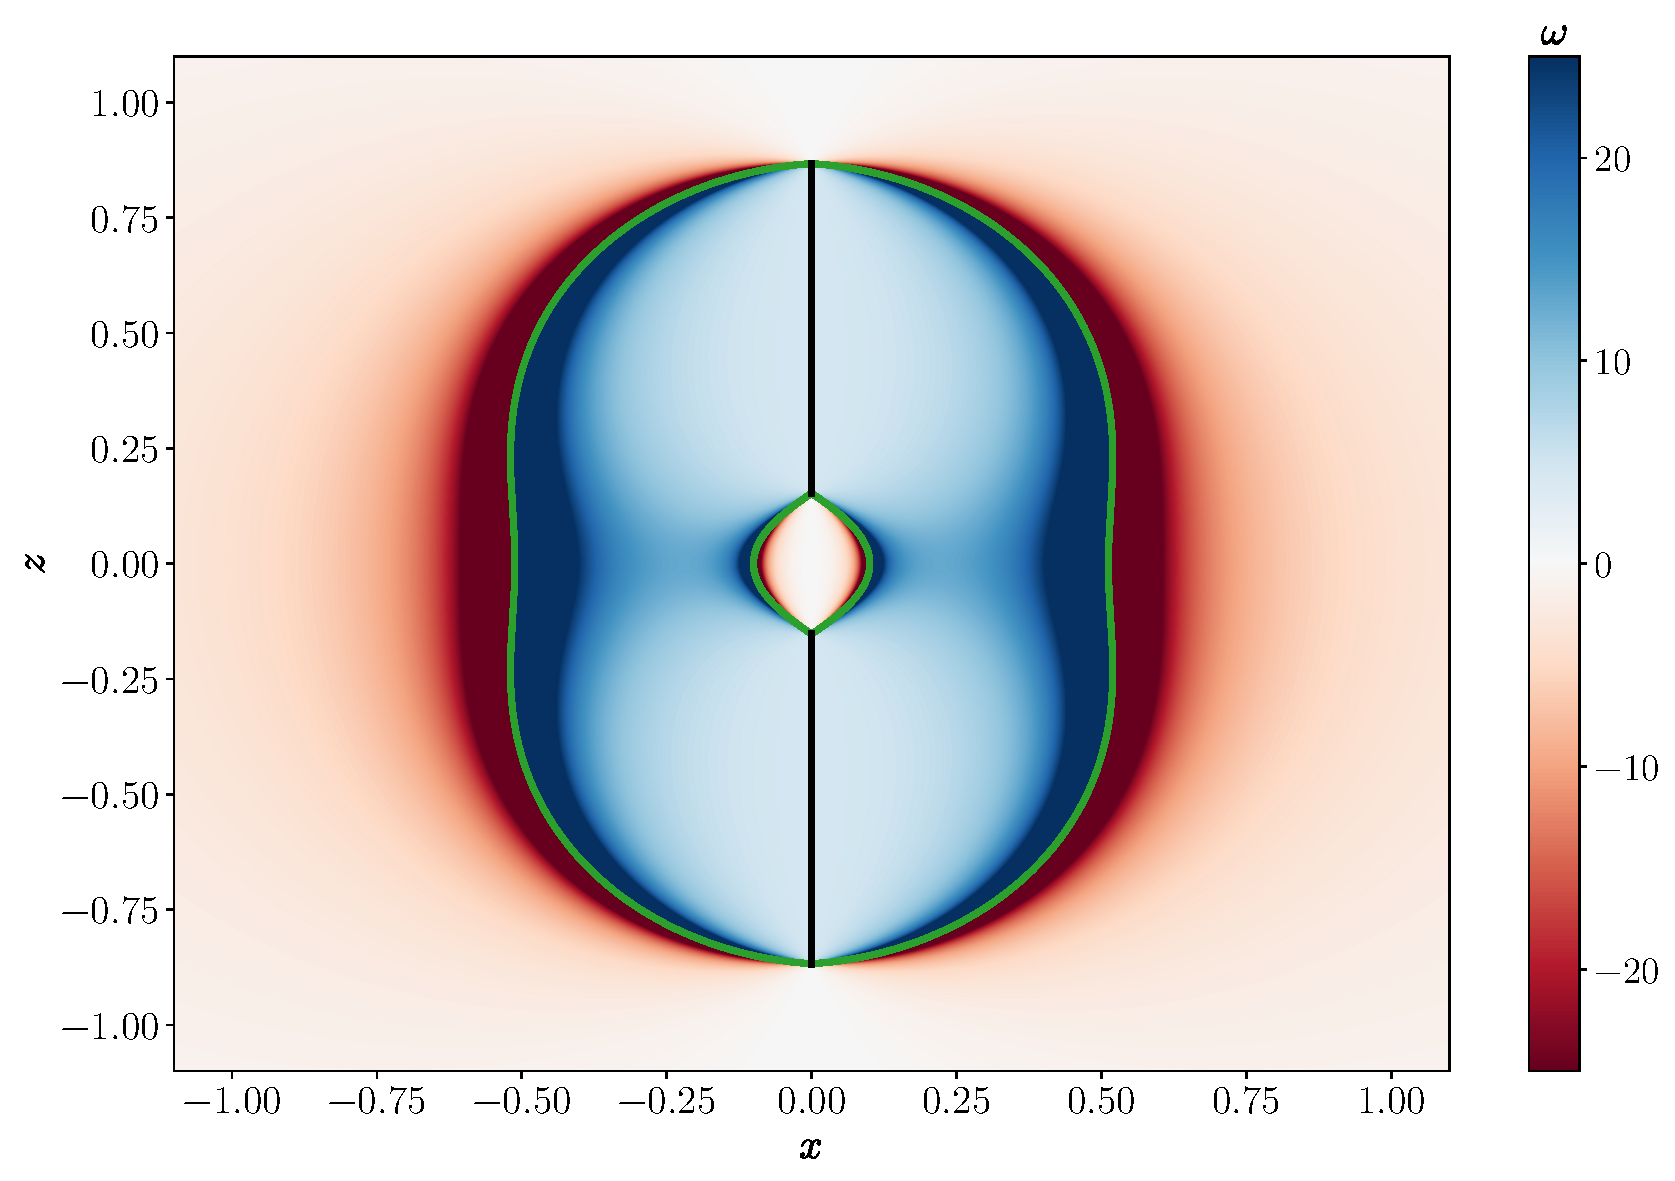
\includegraphics[scale = 0.25]{img/penrose_binaries/cmmr_omega/omega_b_0.98_q_1.0_a1_0.65_a2_0.65.pdf}
    \label{ch:penrose_binaries/fig:omega_dens_a}
  }
  \subfloat[$a_1= -a_2 = -0.65$]{
    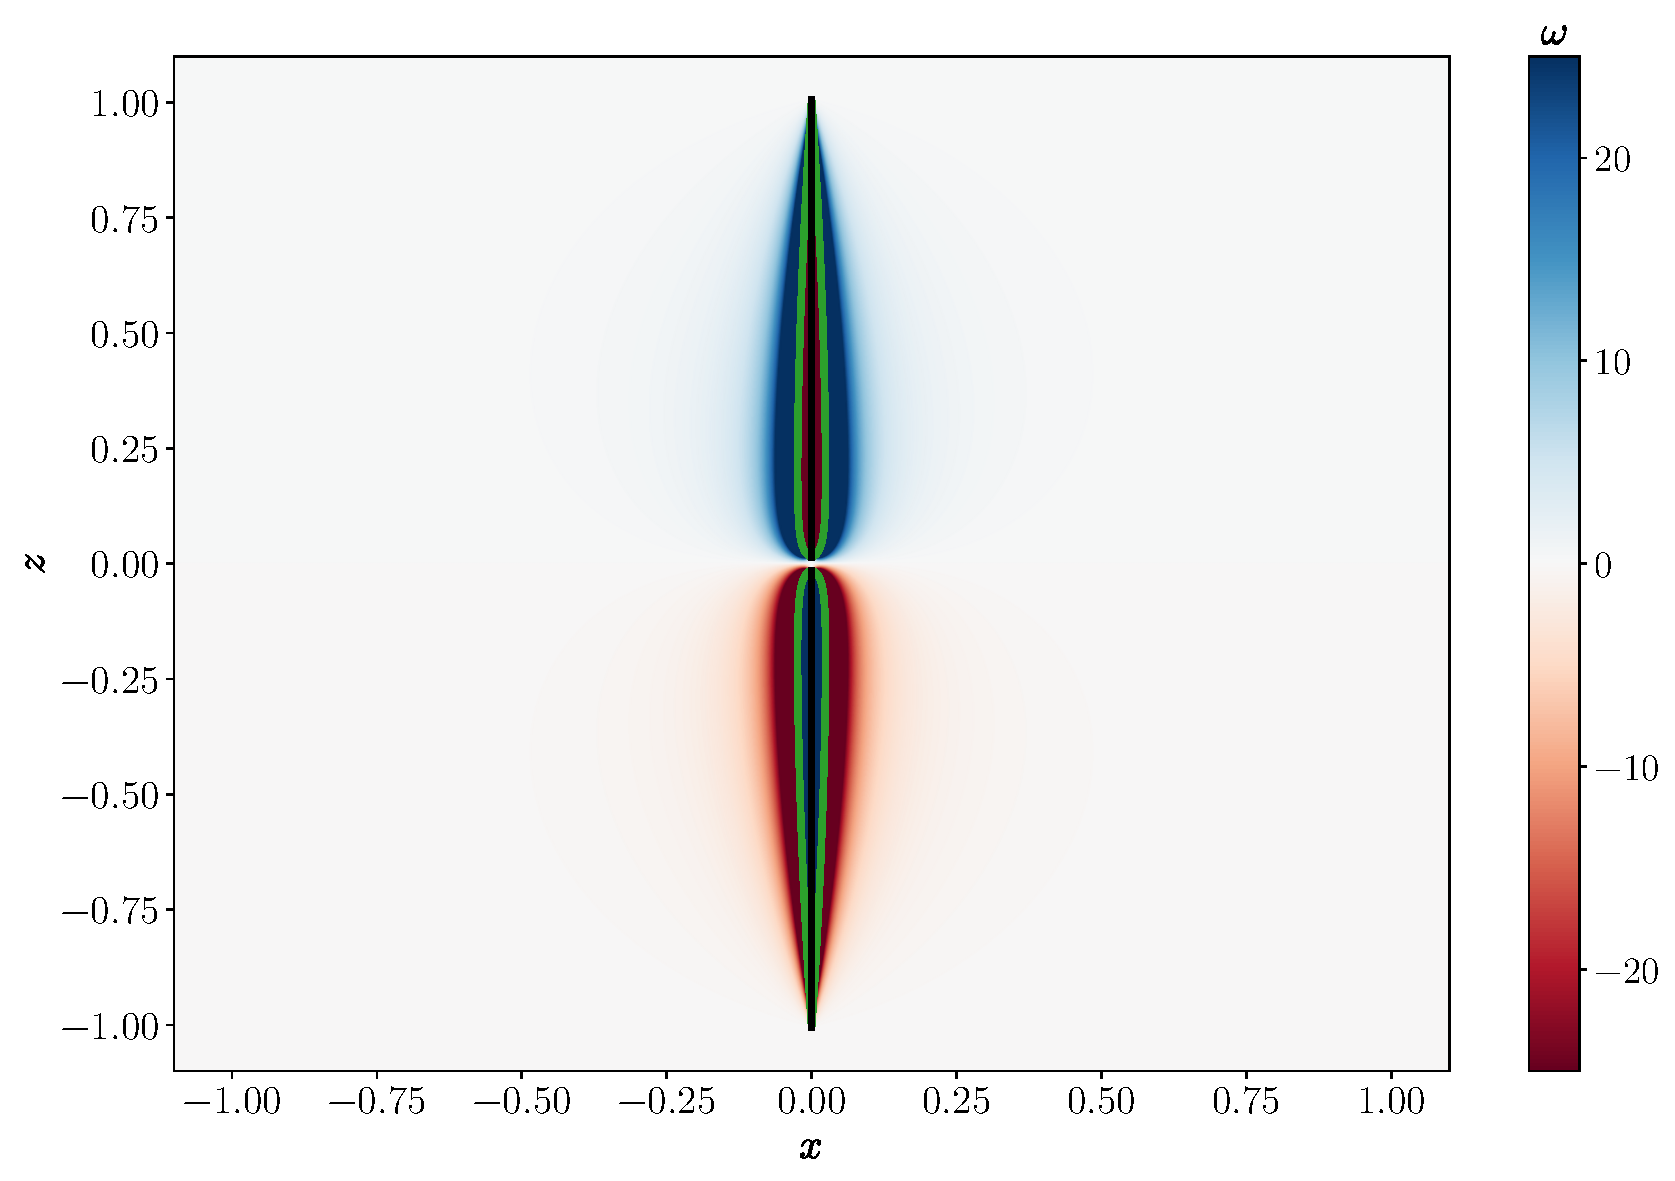
\includegraphics[scale = 0.25]{img/penrose_binaries/cmmr_omega/omega_b_0.98_q_1.0_a1_-0.65_a2_0.65.pdf}
    \label{ch:penrose_binaries/fig:omega_dens_b}
  }
  \newline
  \subfloat[$a_1= 0.65$, $a_2 = -0.1$]{
    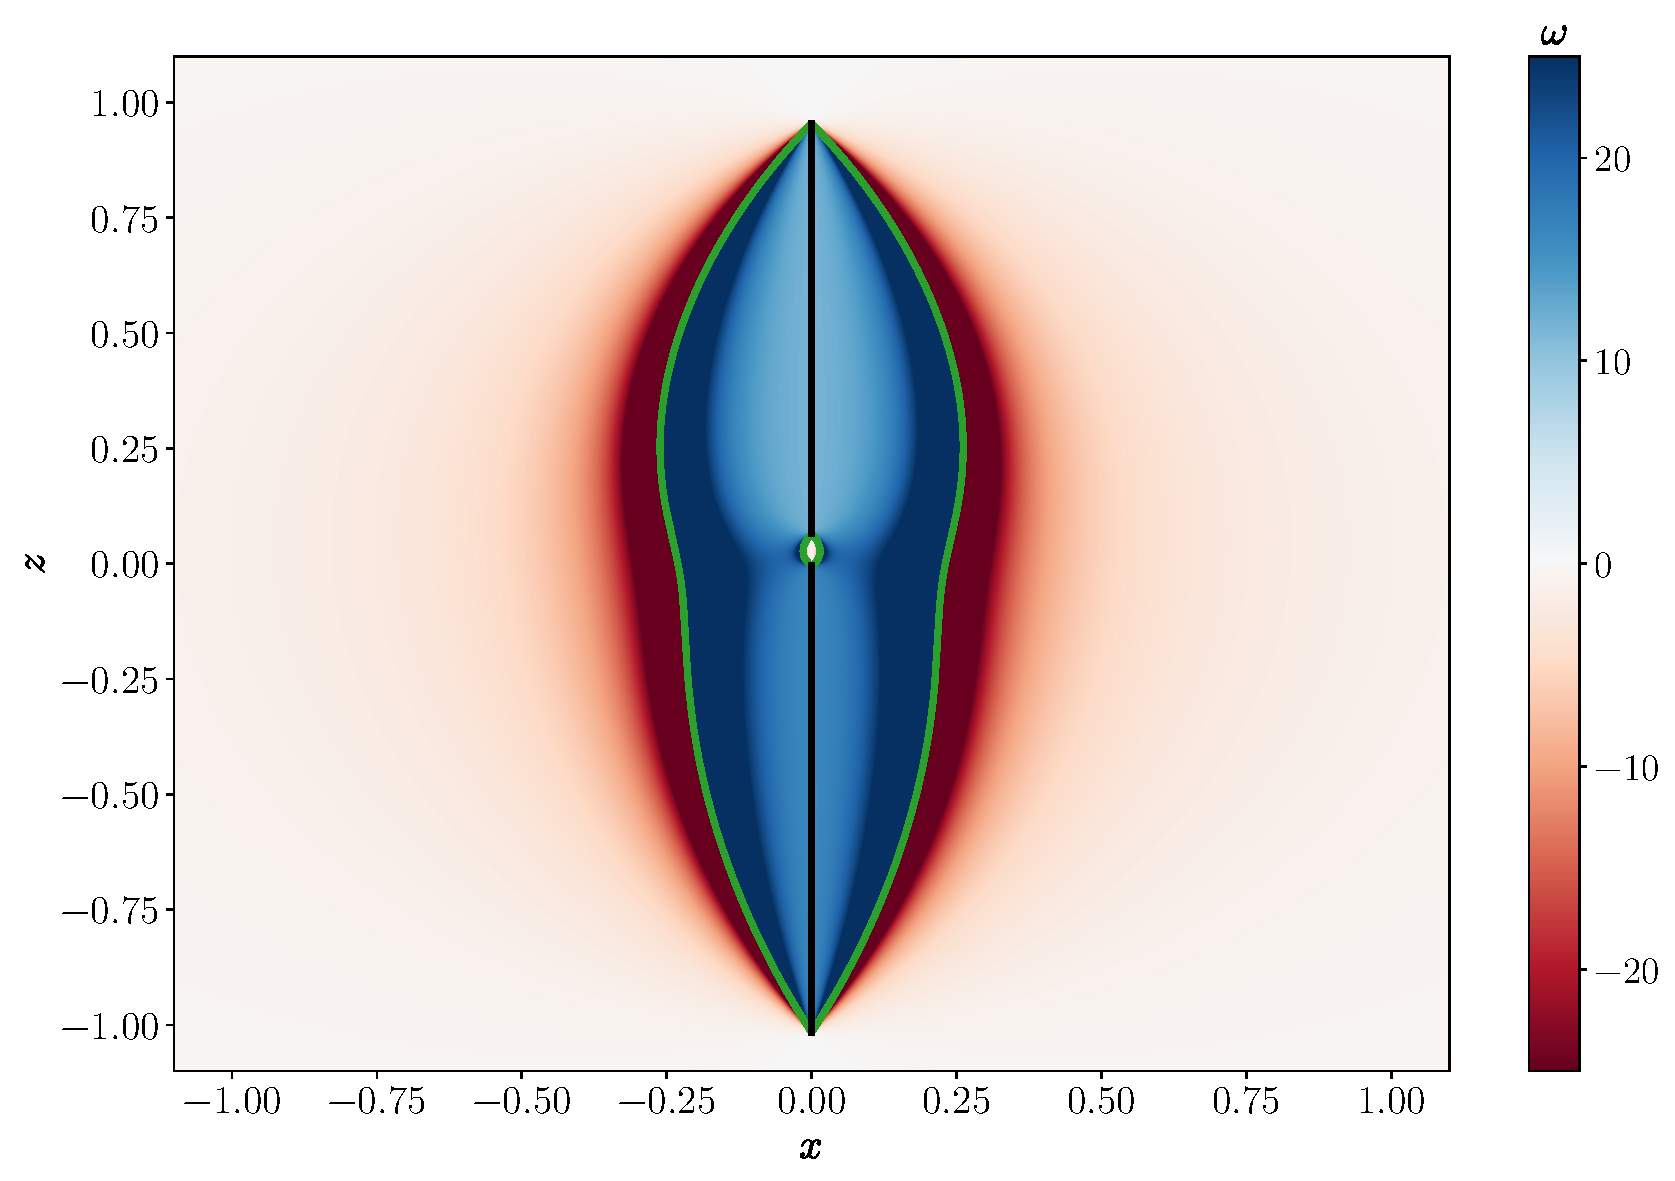
\includegraphics[scale = 0.25]{img/penrose_binaries/cmmr_omega/omega_b_0.98_q_1.0_a1_0.65_a2_-0.1.pdf}
    \label{ch:penrose_binaries/fig:omega_dens_c}
  }
  \subfloat[$a_1= -0.65$, $a_2 = 0.1$]{
    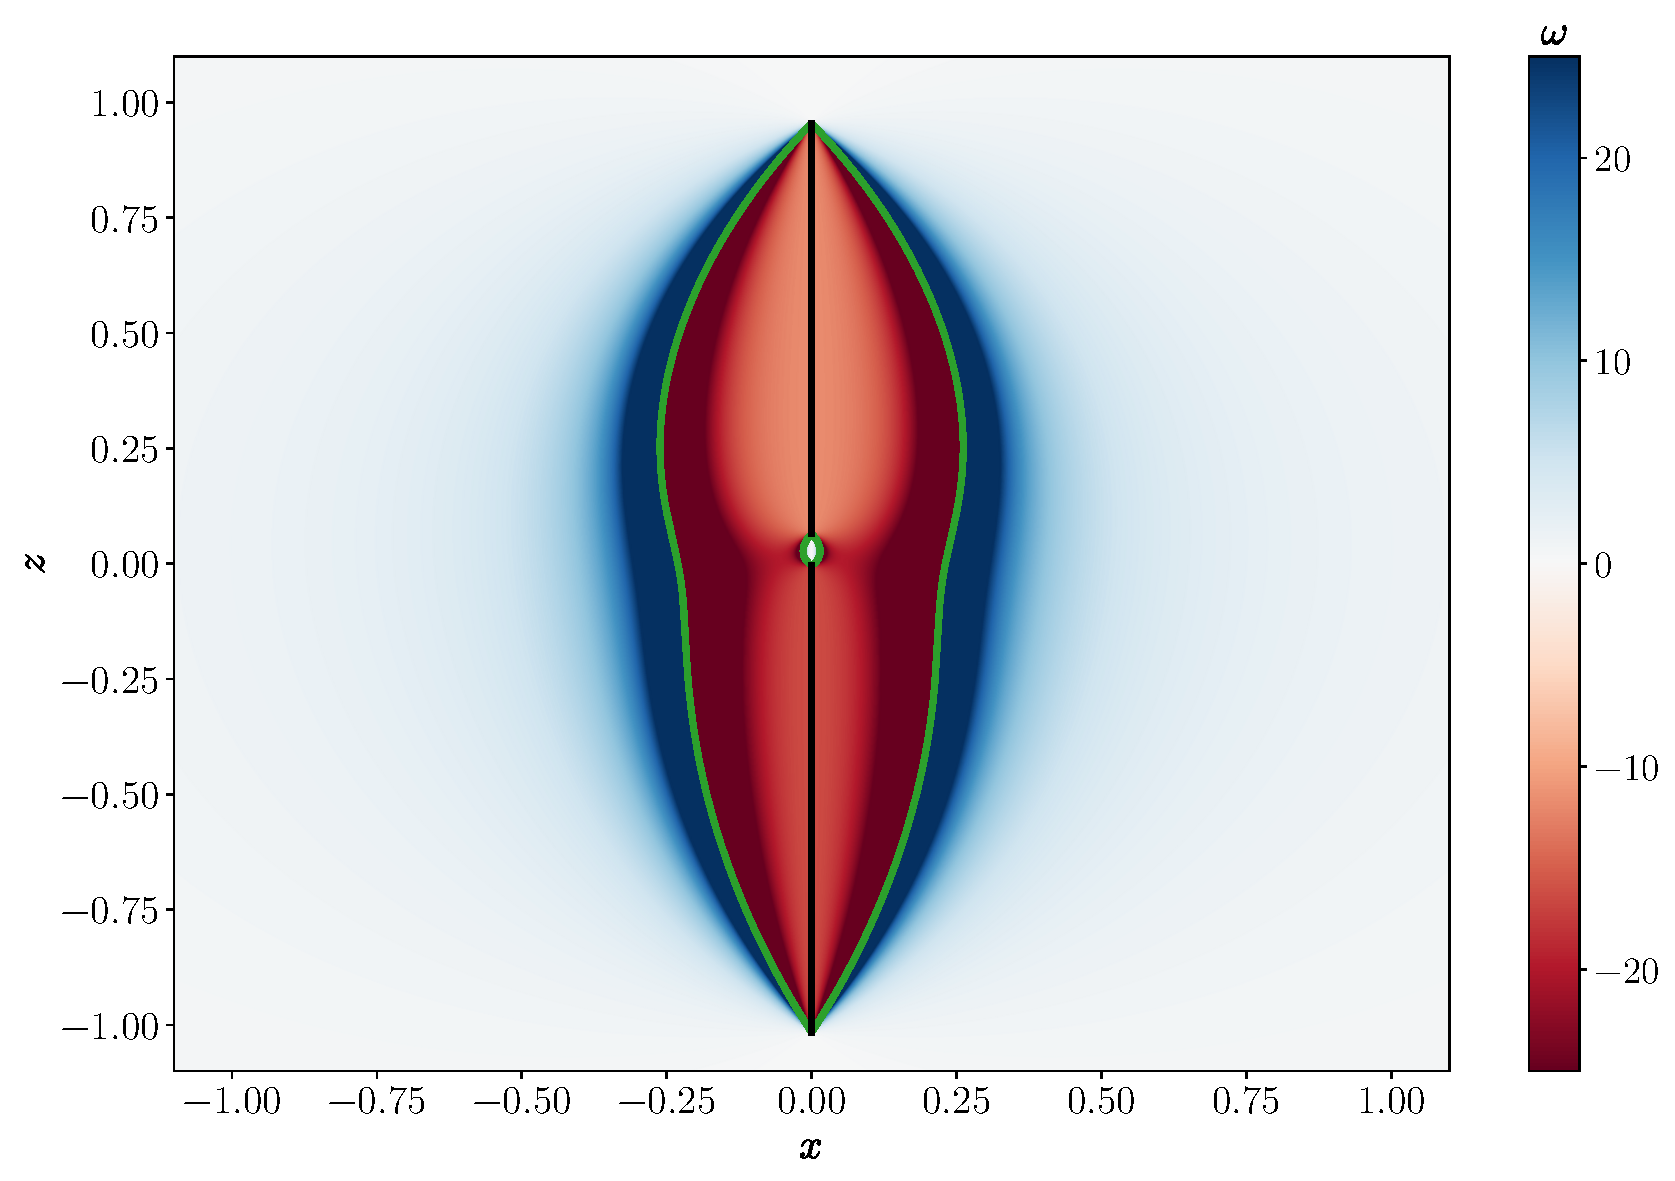
\includegraphics[scale = 0.25]{img/penrose_binaries/cmmr_omega/omega_b_0.98_q_1.0_a1_-0.65_a2_0.1.pdf}
    \label{ch:penrose_binaries/fig:omega_dens_d}
  }
  \caption{The value of $\omega(\rho,z)$ projected in Cartesian coordinates. In all plots $b=0.95$ and $q=1.0$. The green curve marks the limit of the ergospehre and the black lines mark the event horizons.}
  \label{ch:penrose_binaries/fig:omega_value_regions}
\end{figure}

\subsection{Efficiency of energy extraction}

We now turn our attention to the maximum energy that can be extracted from the system by means of the Penrose process. It widely know that no more energy can be extracted than the \textit{irreducible mass} of each black hole~\cite{RUFFINI1971,CHRISTODOULOU1970,carroll}. The irreducible mass $M_{\text{irr}}$ is related to the horizon area $A$ by the well know formula~\cite{carroll}
%
\begin{equation}
  M_{\text{irr}} = \sqrt{\frac{A}{16\pi}}.
  \label{ch:penrose_binaries/eq:irreducible_mass}
\end{equation}
%
The entropies of each black hole in the CMMR metric are know and given in Eq.~(22) of Ref.~\cite{MANKO2020}. Given that the entropy $S$ and horizon area are related by $A=4S$ we have that the maximum energy that can be extracted from the system is the sum of the maximum energy that can be extracted from each hole individually, that is
%
\begin{equation}
  E_{\text{max}} = \left(m_1 - \sqrt{\frac{S_1}{4\pi}}\right) + \left(m_2 - \sqrt{\frac{S_2}{4\pi}}\right).
  \label{ch:penrose_binaries/eq:max_extract_energy}
\end{equation}

In the traditional Penrose process there is only one particle of negative energy and thus only one of the black holes will loose part of it's rotation. In practice this meas that only one of the terms inside the parenthesis of Eq.~\ref{ch:penrose_binaries/eq:max_extract_energy} will contribute to the energy extraction. A remarkable fact is that if one takes the limit of $R \rightarrow \infty$ of one of these terms (e.g. the first) in Eq.~\ref{ch:penrose_binaries/eq:max_extract_energy} one obtains
%
\begin{equation}
  E_{\text{max}} = m_1 - \frac{1}{\sqrt{2}}\left(m_1^2 + \sqrt{m_1^4 - j_1^2}\right)^{1/2}
  \label{ch:penrose_binaries/eq:energy_extraction_kerr_limit}
\end{equation}
%
where we remind that $j_1=a_1m_1$. This expression is exactly the one obtained for the maximum extracted energy in the case of a single Kerr black hole of mass $m_1$ and angular momentum $j_1$~\cite{carroll} which reassures us to the fact that a Kerr binary behaves as a system of isolated Kerr black holes if their separation is large.

\section{Geodesic motion in arbitrary space-times}

In this section we will discuss a method that we intend to implement which would allow us to investigate the Penrose process in arbitrary (even numerically evolved) spacetimes. As we've seen, the Penrose mechanism depends on the existence of orbits that have negative energy according to a static observer far away from the system. If such orbits exist, energy can be extracted from the system. We've also shown that such orbits must lie inside the ergosphere of the binary system, but the notion of ergosphere is not easily generalized to dynamic space-times and remains an open problem. Instead of attempting to define an ergosphere in a dynamical background, we will investigate geodesic motion in such background. The methods and tools for this are already well know in the branch of \emph{ray tracing} in NR for computing the shadows of binary black holes. It all hinges on the ADM (Arnowitt, Deser and Misner) of the geodesic equation.

\subsection{ADM Decomposition of the geodesic equation}

The ADM decomposition, also know as the $3+1$ decomposition is a formulation of GR that rewrite Einstein's field equations as a Cauchy (initial value) problem and is a very common representation of spacetimes used in NR. In this decomposition, the spacetime metric is written as~\cite{BAUMGARTE}

\begin{equation}
  \ud s^2 = -\alpha^2 \ud t^2 + \tens{\gamma}{}{ij} \left( \ud \tens{x}{i}{} + \tens{\beta}{i}{}\ud t\right) \left( \ud \tens{x}{j}{} + \tens{\beta}{j}{}\ud t\right)
  \label{ch:penrose_binaries/eq:adm_metric}
\end{equation}
%
where $\alpha$ is the lapse function, $\tens{\beta}{i}{}$ the shift vector and $\tens{\gamma}{}{ij}$ the spatial metric.

The decomposition of the geodesic equation we will adopt follows Ref.~\cite{BOHN2015} closely. We note that a very similar approach was also develop in Ref.~\cite{VINCENT2012}, which we also refer for additional details. We start by defining the auxiliary variable

\begin{equation}
  \tens{\Pi}{}{i} \equiv \frac{\tens{p}{}{i}}{\alpha \tens{p}{}{0}} = \frac{\tens{p}{}{i}}{\sqrt{\tens{\gamma}{jk}{} \tens{p}{}{j} \tens{p}{}{k}}}
  \label{ch:penrose_binaries/eq:big_pi_def}
\end{equation}
%
where $p^i \equiv \ud x^{i}/\ud \tau$ is the particle's 4-momentum, $x^i$ the spacetime coordinates and $\tau$ the particle's proper time.

Using the ADM decomposition, the geodesic equation can be written as~\cite{BOHN2015}

\begin{align}
  \der{\tens{\Pi}{}{i}}{t} =          & -\indexdel{i}\alpha + \left[ \left( \indexdel{j}\alpha \right) \tens{\Pi}{j}{} - \alpha \tens{K}{}{jk} \tens{\Pi}{j}{} \tens{\Pi}{k}{}\right]\tens{\Pi}{}{i} + \left( \indexdel{i}\tens{\beta}{k}{} \right) \tens{\Pi}{}{k} - \frac{1}{2} \alpha \left( \indexdel{i} \tens{\gamma}{jk}{} \right) \tens{\Pi}{}{j} \tens{\Pi}{}{k} \\
  \der{\tens{x}{i}{}}{t} =            & \alpha \tens{\Pi}{i}{} - \tens{\beta}{i}{}                                                                                                                                                                                                                                                                                       \\
  \der{\ln(\alpha\tens{p}{0}{})}{t} = & -\left( \indexdel{i} \alpha \right) \tens{\Pi}{i}{} + \alpha \tens{K}{}{ij}\tens{\Pi}{i}{}\tens{\Pi}{j}{}
  \label{ch:penrose_binaries/eq:adm_geodesic_eq}
\end{align}
%
where $t$ is the coordinate time, $\tens{K}{}{ij}$ is the extrinsic curvature and $\tens{\Pi}{i}{} = \tens{\gamma}{ij}{}\tens{\Pi}{}{j}$.
\subsection{Observed quantities}
\subsection{Proposal for investigating the Penrose process in numeric space-times}